%%%%%%%%%%%%%%%%%%%%%%%%%%%%%
%ES100 Latex Template
%Sam Meijer '19
%Hopefully this template will serve you well.
%It is built off many other packages and templates, but I have added my own style here and there, as you should too!
%I will endeavour to explain some of the intricacies of LaTex as well as how to lay out an overall project.
%Hopefully no knowledge of LaTex is required to understand this document.
%I would highly recommend https://www.overleaf.com/learn/latex/Main_Page for further information.
%For errata, please contact smeijer11@gmail.com.
%%%%%%%%%%%%%%%%%%%%%%%%%%%%%

%Packages are included below, these are akin to libraries in other programming languages. As far as I can tell, there is no reason to reduce the number of packages included in a document. It might compile faster, but overleaf compiles fast so this should not be an issue.
\documentclass[12pt,twoside]{report} %tells the compiler that this is a 'report' style document, and the main font size.
\usepackage{setspace} %allows the use of '\doublespace' to set line spacing
\usepackage[utf8]{inputenc} %inclusion of this is optional, overleaf includes it in its compiler so it is not necessary, it may be necessary for other compilers.
\usepackage[english]{babel} %this does a few things eg allowing dates to be made by the compiler. probably best not to get rid of it
\usepackage{wrapfig} %if it is desirable to wrap text (see https://www.overleaf.com/learn/latex/Wrapping_text_around_figures).
\usepackage{graphicx} %this allows graphics to be put in easily
\usepackage{float}%this allows you to put them in good places
\usepackage[version=4]{mhchem} %this is good for chemical reactions
\usepackage{amsmath} %maths package
\usepackage{amssymb} %symbol package
\usepackage{textcomp,gensymb} %more symbols (eg \degree)
\usepackage{appendix} %self explanatory
\usepackage{colortbl} %good for colouring in cells on a table
\usepackage{rotating} %allows you to rotate graphics
\usepackage{bm} %helps bold things
\usepackage{multirow} %for tables
\usepackage{longtable} %for long tables
\usepackage{booktabs} %more tables
\usepackage{pdfpages} %allows PDFs to be included in document (good if you want to include a pdf in an appendix eg)
\usepackage{caption} %allows captions for graphics
\usepackage[nottoc]{tocbibind} %adds the bibliography to the table of contents
\usepackage{subcaption} %allows subcaption for multiple images in one graphic

\PassOptionsToPackage{hyphens}{url}\usepackage{hyperref}
\usepackage{hyperref} %this is great for putting hyperreferences in the document.
\usepackage[table]{xcolor} %more colouring of tables
\definecolor{Gray}{gray}{0.9} %this defines a colour to be used and gives it a name. This is a colour called 'Gray' it is 'gray' with transparency 0.9

\hypersetup{colorlinks=false} %this stops links being colourful, which makes a report look less professional I believe.

\usepackage[letterpaper, top=1in, bottom = 1in, right = 1in]{geometry} %this describes the layout of the document and the margins etc.
\doublespacing %self explanatory

\begin{document} % you have to do this to start the document

%%%%%%%%%%%%%%%%%%%%%%%%%%%%%%%%%%%%%%%%%%%
%For a long report such as a thesis, I would recommend thinking like programming, that is, have a short 'main' and long programs (or chapters in this case) this allows you to access each chapter easily and see the layout of the document easily.
%
%using \input{} basically puts the code specified in the argument (between the braces) into the body of the code in main
%%%%%%%%%%%%%%%%%%%%%%%%%%%%%%%%%%%%%%%%%%%

% The entire thesis is generated by the commands below, referencing the other files in this directory.

%%%%%%%%%%%%%%%%%%%%%%%%%%%%%%%%%%%%%%%%%%%
% MY PREAMBLE
%%%%%%%%%%%%%%%%%%%%%%%%%%%%%%%%%%%%%%%%%%%

\begin{titlepage}
    \begin{center}
        \vspace*{1cm}
        % this title page can be played around with to better serve your project. the necessary parts to include are the TITLE at the top, the BLURB about the thesis presented etc. Name, faculty member, date, type of engineering...
        \begin{figure} [H]
            \centering
            
\includegraphics[width=0.8\textwidth]{Images/tail0r wordmark.png}
        \end{figure}
        
        \Huge
        \textbf{tail0r: \\ Towards Custom-Sized, Zero Waste Garments using a Computational Framework}

 
        \vspace{1.5cm}
 
 
        \vfill
        
        
        \textbf{Rohil J Dave}
 
        \vspace{0.8cm}
 

 
        \Large
        MEng Degree Candidate in Design Engineering\\
        Supervisor: Dr Rebecca Stewart\\
        Imperial College London Dyson School of Design Engineering\\
        London UK\\
        6 June 2024
 
    \end{center}
\end{titlepage}

\pagenumbering{roman} %Roman numbering is recommended until the body

\tableofcontents 

% \listoffigures 

% \listoftables 

\chapter*{Abstract}

This report focuses on reducing waste during garment manufacturing, where \~15\% of all fabric is wasted. Designs with increased garment utility and desirability are explored. ‘Zero waste patterns’ are one such class of designs. This study looks at parameterisation of these patterns based on individual body measurements and suggests mitigation techniques like embellishments. New tools that allow end users to visualize drape and fit of the 2D patterns in 3D are investigated.

These parameterisation heuristics are tested in a workshop setting and participants’ responses to ease of tailoring as well as suitability and fit of the design are collated. Lastly, these patterns are tested on a publicly available data set of scanned body measurement and efficiencies (minimised fabric loss) were computed for industry standard bolt widths. 

% This section needs to be reworkeds 

\pagenumbering{arabic} %back to Arabic numbering for the rest

%%%%%%%%%%%%%%%%%%%%%%%%%%%%%%%%%%%%%%%%%%%
% MY CHAPTERS
%%%%%%%%%%%%%%%%%%%%%%%%%%%%%%%%%%%%%%%%%%%

\chapter{Introduction}

This introduction section will provide an overview of the sustainability crisis, outline the project's focus within the problem, and contextualize the following literature review.

\section{Sustainability Crisis in the Fashion Industry}
The fashion industry is a significant contributor to environmental degradation, second only to oil and mining. Waste and inefficiencies are endemic over the entire lifecycle. 
\subsection{Sourcing and Processing}
The problem starts from yarn production whether harvesting natural materials like cotton or the production of synthetic fibres. For example, cotton farming uses pesticides and fertilizers that pollute soil and water, leading to disasters like the Aral Sea shrinkage, while polyester production emits greenhouse gases and microplastics, harming marine life and human health. Furthermore, dyeing and finishing processes in textile manufacturing release harmful chemicals into water bodies, affecting aquatic ecosystems and human health. According to the Ellen MacArthur Foundation, the industry is responsible for approximately 10\% of global carbon emissions and is the second-largest consumer of the world's water supply.
\begin{figure} [H]
    \centering
    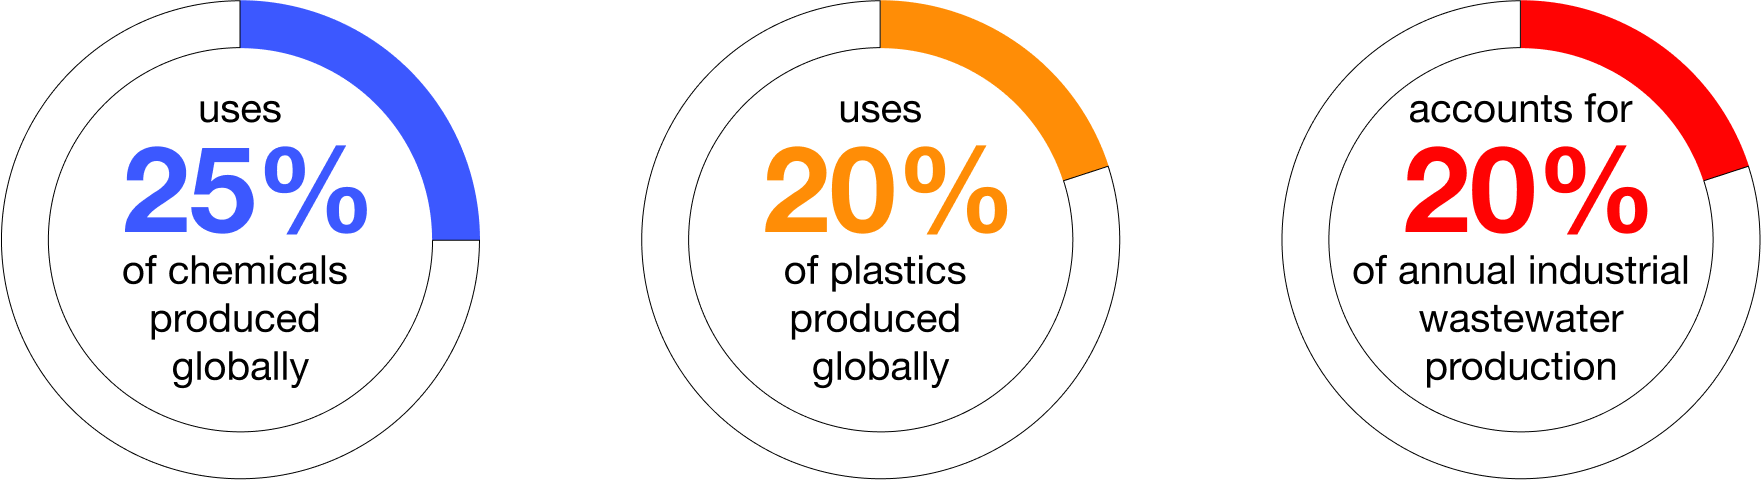
\includegraphics[width=0.8\textwidth]{Images/sourcing donuts.png}
    \caption{Fashion industry consumption metrics}
\end{figure}
\subsection{Overproduction and Overconsumption}
The fast fashion business model results in a relentless cycle of overproduction and overconsumption. Brands rapidly produce large quantities of low-cost, low-quality garments to chase ever-changing trends and induce consumer demand. Estimates suggest that by 2050, annual garment production will reach a staggering 814 billion garments, with a cumulative total of over 9.5 trillion garments produced from now until then. Social pressure to frequently update wardrobes undermines eco-conscious consumerism, fostering a throwaway culture, where clothing is discarded after only a few uses. During garment production, an average of approximately 15\% of fabric per garment is wasted during the cutting process. Thus, the resulting unsustainability is multi-dimensional: cut losses are often not recycled, unsold inventory is discarded, and consumers quickly dispose of their purchases. Pan describes this as a 'wicked problem' plagued by short product life cycles and excessive waste.

\section{Project Focus}
Within the fashion supply chain, this project focuses at the garment manufacturing stage and how to reduce waste both pre and post the point of sale. This is a question of material efficiency but also of what makes a garment desirable and why people might value it on an individual level. 

The project will explore the concept of 'zero waste patterns' and how they can be parameterised based on individual body measurements. The aim is to create designs that are both sustainable and desirable, increasing garment utility by recouping fabric cut loss. This will involve exploring the principles of zero waste pattern making, bespoke clothing, and garment utility, and how these concepts can be integrated into the design process. 

% The project will also investigate new tools that allow end-users to visualise the drape and fit of 2D patterns in 3D, enabling them to make more informed decisions about their clothing purchases.  DO WE ALSO WANT TO INCLUDE HERE HOW THE PROJECT WILL BE EVALUATED?

\chapter{Literature Review}
This literature review surveys fabric waste at the point of garment manufacturing, examines traditional pattern making processes, the advent and principles of zero waste design, the methods and rationale behind bespoke clothing, the concept of garment utility, and the impact of digitisation trends on these processes. By analysing these aspects, the review seeks to provide a comprehensive understanding of the current challenges in reducing fabric waste and how innovative solutions that promote sustainable practice in the fashion industry can be used.

\section{Fabric Waste During Garment Manufacturing}
Fabric waste occurs at various stages of the manufacturing process, including cutting, sewing, and finishing. The cutting stage is particularly problematic, as patterns are not always optimised for fabric efficiency. On average, approximately 15\% of fabric per garment is wasted during production, with some instances reaching nearly 30\% \cite{black_sustainable_2013}. The rigidity of traditional pattern making limits creativity and innovation, making it difficult to adapt to new sustainable practices, particularly on industrial scales.

The hierarchy of waste management options (Figure \ref{fig:waste_hierarchy}) can be applied to the fashion industry. This project is concerned with the more favoured options of prevention, minimisation, and reuse. Rissanen analogises that cutting fabric pieces is like cutting cookies from rolled dough; however, unlike dough, fabric scraps cannot be reformed into material of the same quality \cite{rissanen_zero-waste_2013}. Dimensions of fabric scraps constrain reuse possibilities. Therefore, this project focuses on preventing waste from the fabric source and minimising it where possible through reuse.
\begin{figure} [htb]
    \centering
    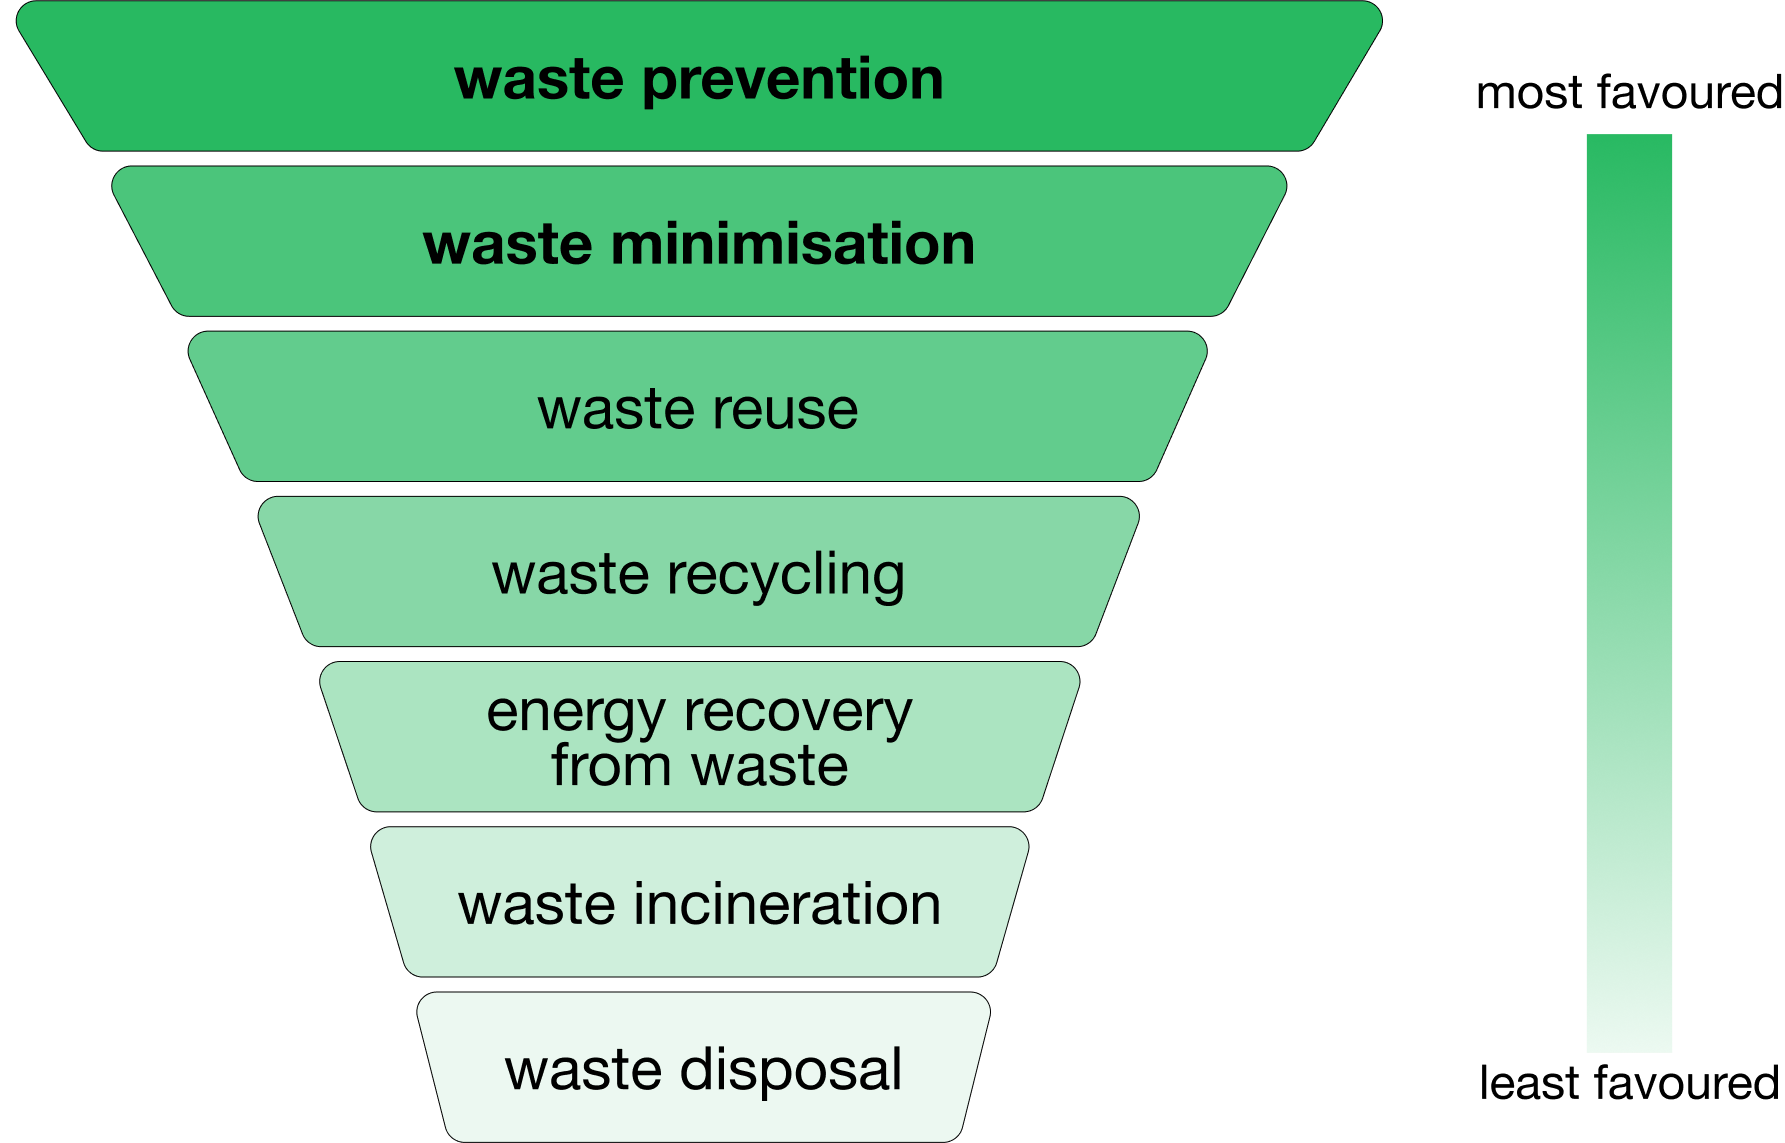
\includegraphics[width=0.6\textwidth]{Images/waste hierarchy.png}
    \caption{Waste management hierarchy \cite{rissanen_zero-waste_2013,mcdougall_integrated_2001}}
    \label{fig:waste_hierarchy}
\end{figure}

In the context of recouping fabric, designers should consider garment utility. Enhancing garment utility can involve incorporating fabric cut loss reduction into the garment's design in creative ways, simultaneously increasing the garment's overall appeal and lifespan. This is a core principle of `slow fashion', which advocates for mindful consumption and long-term use of clothing. By focusing on garment utility, designers can create more sustainable fashion products that meet consumer demands and address the cutting floor's environmental impact.

\section{Traditional Pattern Making}
Traditional pattern making involves the creation of two-dimensional templates for cutting fabric pieces of a garment. This manual process, outlined in Figure \ref{fig:traditional_making_flow}, includes several critical steps. In industrial settings, these roles are carried out by different specialists. First, a designer creates a fashion sketch. A patternmarker then interprets the sketch into pieces, drafting a basic pattern block from specifications and measurements. Once this is established, grading is used to scale the pattern to different sizes, adding or subtracting specific amounts at strategic points to maintain the proportions of the original design. A marker-maker subsequently creates a marker, a layout of pattern pieces on fabric. Finally, the fabric is cut, and the pieces given to a sewer to assemble the garment. In smaller-scale or independent practices, however, the same person may perform multiple or all these tasks, necessitating a broad skill set and understanding of each role. This versatility contrasts with the specialisation seen in larger-scale operations.
\begin{figure} [htb]
    \centering
    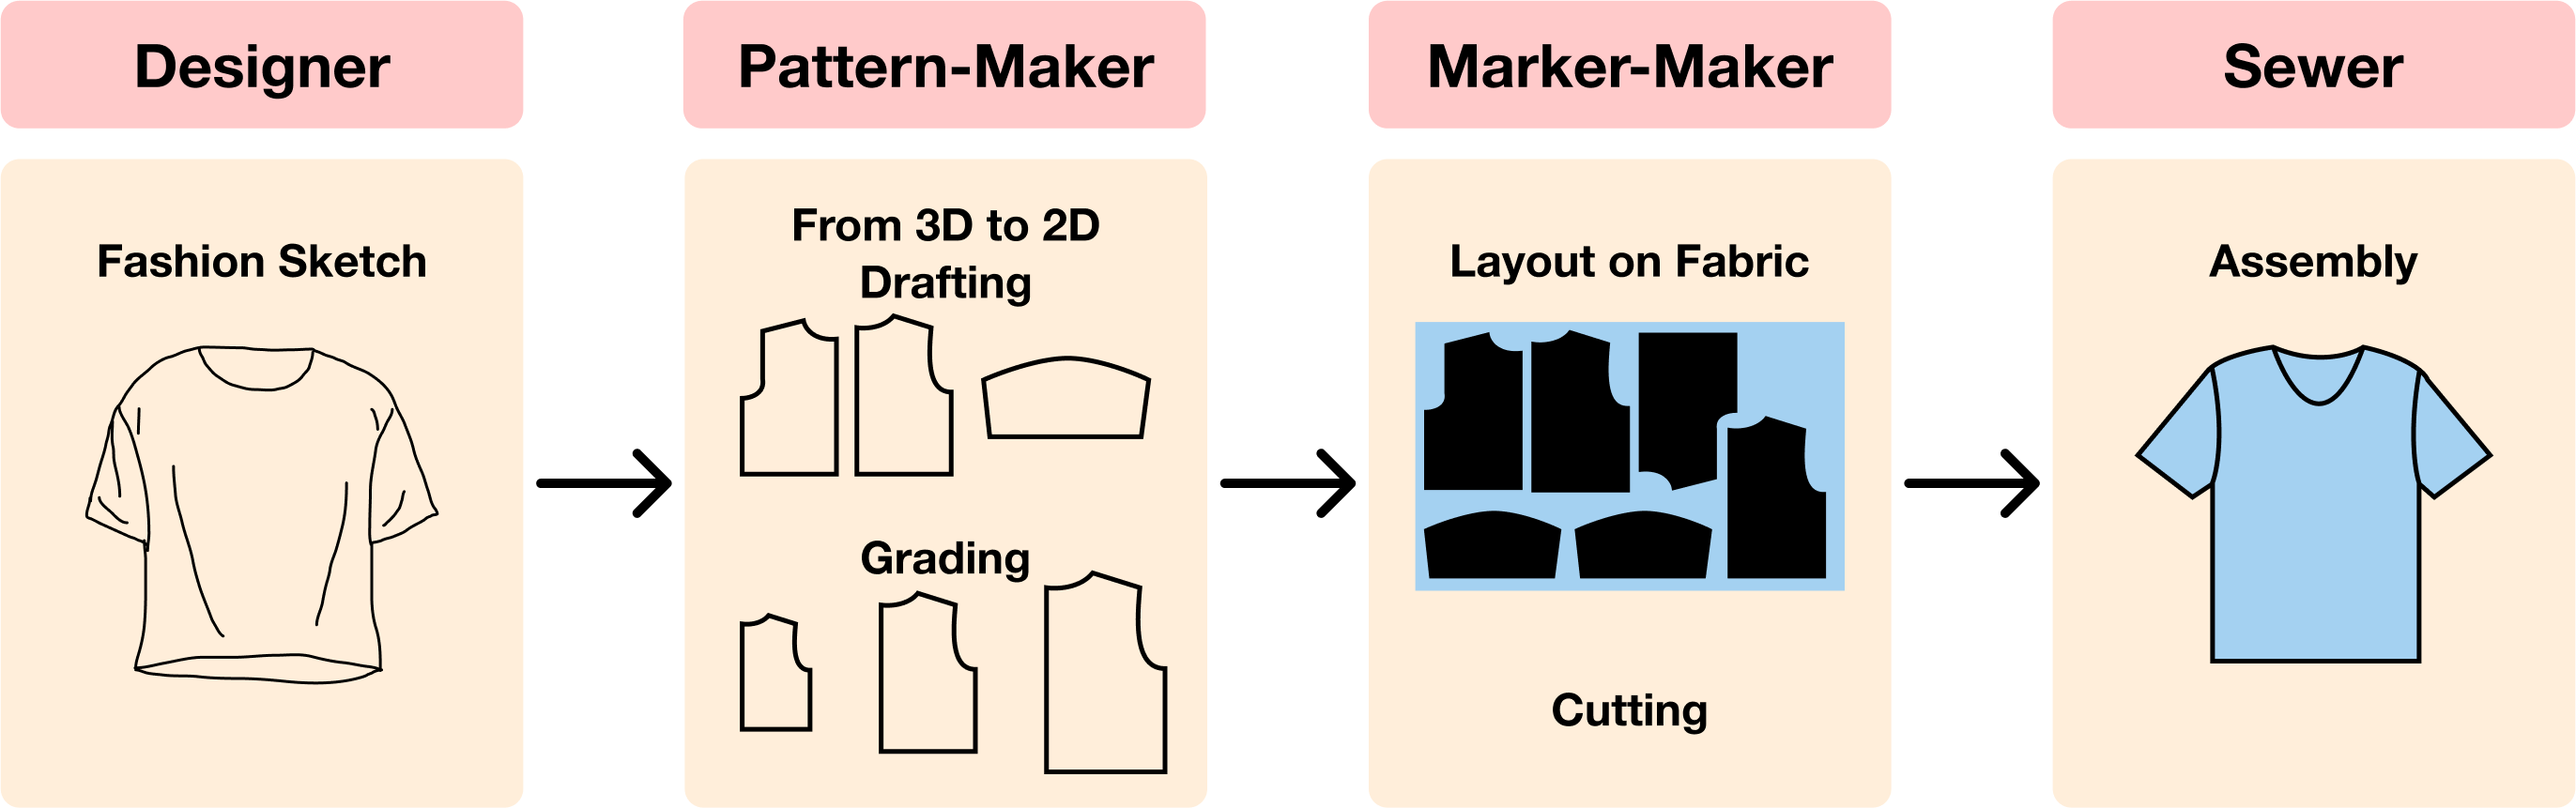
\includegraphics[width=\textwidth]{Images/pattern make diagram.png}
    \caption{Traditional pattern making flow}
    \label{fig:traditional_making_flow}
\end{figure}
Grading has been criticised for its lack of inclusivity, as it often does not accommodate diverse body shapes and sizes. Examples abound of `big/tall' sizes, `petite' sizes, and size nomenclature devoid of specific body measurements (e.g., `women's size 6'). The challenge lies in the fact that human proportions do not scale uniformly, making it impossible to apply a universal rule to pattern scaling. Various approaches, such as manual grading, rule-based grading, and computer-aided design grading, attempt to address this issue, but none can universally adapt a pattern to all body types. Often, manufacturers do not produce clothing in all sizes for branding or inventory reasons, further limiting consumer choice. This lack of inclusivity underscores the complexity and limitations of current grading systems in addressing the diversity of human body shapes.

While effective for mass production, traditional methods often result in significant fabric waste. Traditional pattern pieces placed on a marker are cut out separately, surrounded by negative space. This separation often results in pieces not sharing borders, leading to unusable offcuts. Even with advanced software (Figure \ref{fig:digital_marker_layout}) and skilled manual marker-makers, fabric wastage remains north of 10\%. Fletcher critiques the fact that waste minimisation is not integrated into the design phase, highlighting that the industry accepts these losses as an acceptable and inevitable part of the supply chain.
\begin{figure} [htb]
    \centering
    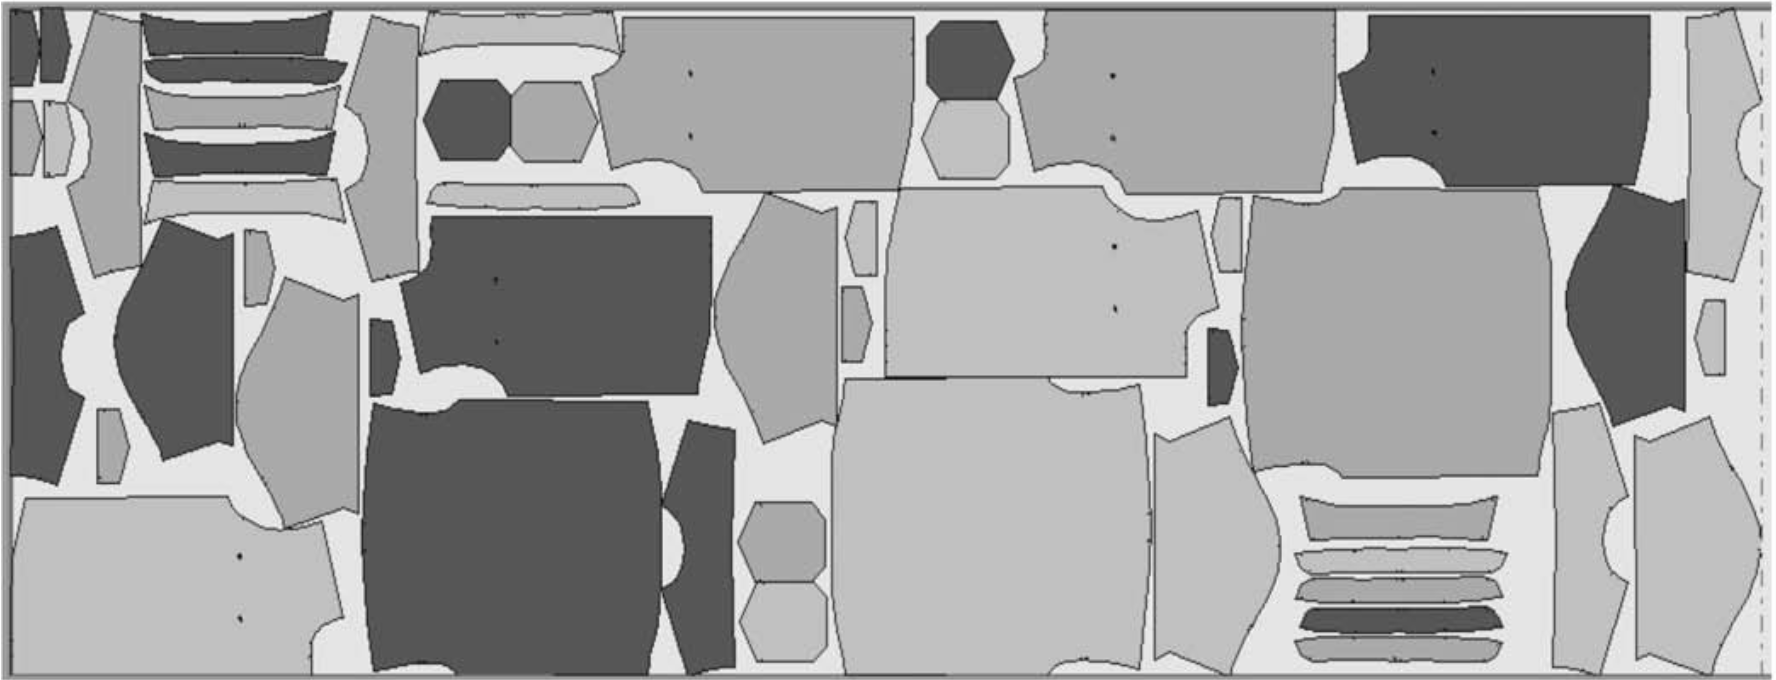
\includegraphics[width=0.75\textwidth]{Images/digital marker layout.png}
    \caption{TukaTech digital marker \cite{joseph-armstrong_patternmaking_2014}}
    \label{fig:digital_marker_layout}
\end{figure}

\section{Zero Waste Pattern Making}
\subsection{Paradigm Shift}
Zero waste pattern design represents a paradigm shift in addressing fabric waste, constrasting sharply with traditional methods. This approach requires reimagining all conventional tailoring and textile techniques, with the fashion designer and patternmaker acting as one. As per Rissanen, the aim is to ``design a set of garment pieces that take up a given length of fabric in two dimensions...and the garment in three dimensions \cite{fletcher_fashion_2012}." Pattern making is pushed to its extremes as garment pieces are designed to fit together seamlessly, like a `jigsaw puzzle,' to ensure no material is wasted \cite{fletcher_fashion_2012,fletcher_sustainable_2014,black_sustainable_2013,rissanen_zero-waste_2013,mcquillan_zero_2020}. Incorporating fabric that would typically be wasted into the garment design effectively enhances material utilisation without increasing costs \cite{fletcher_sustainable_2014}. Proponents of minimum-waste and zero-waste garment design deem passive participation in the existing system as insufficient and recognise this method demands continuous innovation and experimentation \cite{black_sustainable_2013}.

\subsection{Techniques}
The effectiveness of zero-waste cutting is highly dependent on the designer's creativity and problem-solving skills. There are no universal sets of rules or formulas for creating zero waste patterns, as each design and context presents unique challenges. Moreover, because pattern pieces share borders, traditional pattern grading cannot be applied due to the complex relationships between pieces on the pattern \cite{carrico_inquiry_2022}. Imagination is crucial in navigating the constraints of fabric width and pattern interlocking to create functional and aesthetically pleasing garments.

Lei and Li present three techniques to improve zero-waste pattern design: One-piece Manipulation (OM), Segmentation and Reconstruction (SR), and Fabric Elasticity Application (FEA). OM forms the garment from a single piece of fabric, adjusting excess material with fitting devices like pleats and darts. SR involves breaking fabric into interlocking pieces that are reconstructed to form the garment, allowing for flexible design adjustments and repurposing excess fabric. FEA relies on the fabric's natural stretch properties to fit the body without additional cuts \cite{lei_pattern_2021}.

Effective zero-waste pattern techniques utilise simple shapes, modularity, symmetry, and tessellation to fit the entire pattern into a compact rectangle. Depending on the fabric bolt, offcuts are either eliminated or come in rectangular shapes that are much easier to repurpose \cite{helmersson_zero_2023}. Designers often use these offcuts in embellishments and mendings, adding new features to the garment \cite{}.

\subsection{Application in Small-Scale Domains}
Small-scale practices like independent fashion designers are currently leading the way in adopting zero-waste techniques, as companies are not yet making zero-waste garments for the mass market. While large-scale industry production often overlooks fabric efficiency, smaller-scale operations can experiment with and implement zero-waste designs more flexibly. This flexibility allows them to contribute to a reduction in fabric waste at a grassroots level. By integrating zero-waste principles, independents and small volume producers can create unique, sustainable garments that challenge the norms of traditional fashion design and potentially transform their practices into successful businesses.

\subsection{Design Ease Aesthetic}
Because of simpler, modular shapes, zero waste garments are typically boxy and loose fitting with greater ease around the body. Ease is the difference between body measurements and garment measurements, and it significantly affects fit, comfort, and style. There are two types of ease: wearing ease and design ease. Wearing ease is the minimum amount of extra fabric needed to allow comfortable movement, while design ease involves additional fabric for aesthetic purposes \cite{tessa_what_2022}. Zero waste pattern designs typically incorporate larger design ease to achieve their intended loose-fit aesthetic. This aesthetic is clearly seen in the examples below.

\subsection{Examples}
Here are some visuals to showcase aspects zero waste design process. Rissanen's Endurance Shirt II pattern in Figure \ref{fig:endurance_shirt} shows how he aims to fit pieces compactly into rectangular forms. As seen in Figure \ref{fig:SR_kimono}, excess fabric is repurposed for functional embellishments like pockets and cuffs, which helps in minimising waste and enhancing the garment's utility. Figures \ref{fig:rissanen_jacket} and \ref{fig:bh_tee} highlight the boxy and loose-fitting aesthetic of their resulting designs.

\begin{figure} [H]
    \centering
    \rotatebox{270}{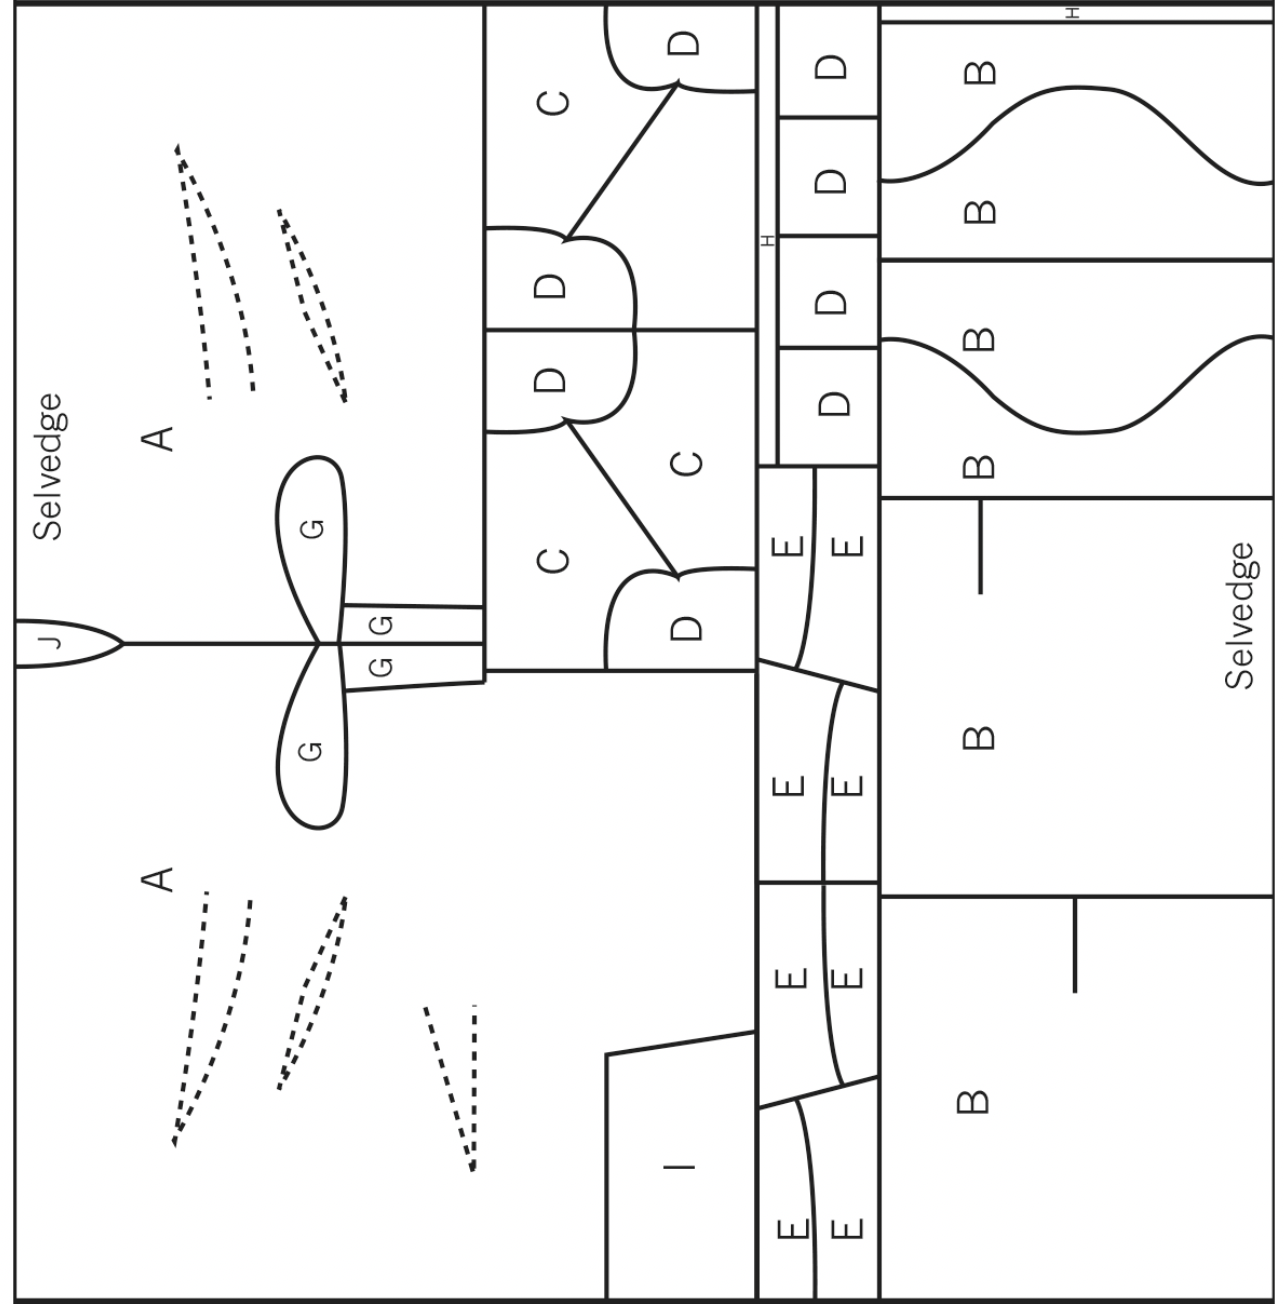
\includegraphics[width=0.8\textwidth]{Images/endurance shirt ii.png}}
    \caption{Endurance Shirt II pattern \cite{fletcher_sustainable_2014}}
    \label{fig:endurance_shirt}
\end{figure}
\begin{figure} [H]
    \centering
    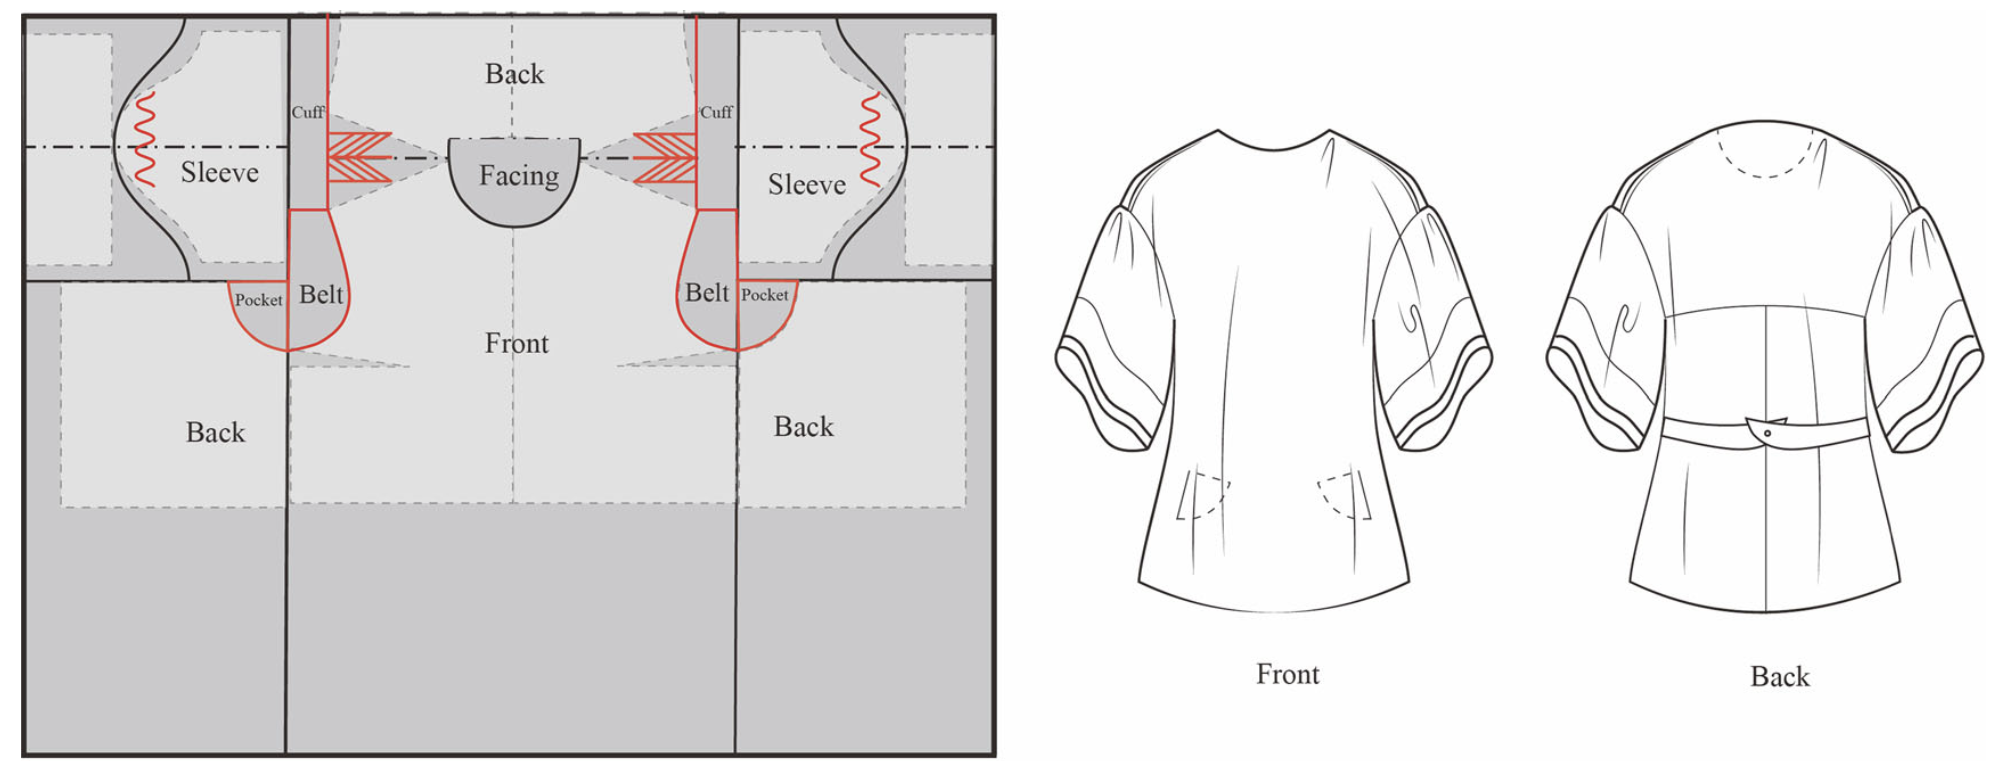
\includegraphics[width=\textwidth]{Images/SR kimono.png}
    \caption{SR kimono pattern and sketch \cite{lei_pattern_2021}}
    \label{fig:SR_kimono}
\end{figure}
\begin{figure} [H]
    \centering
    \begin{subfigure}[b]{0.55\textwidth}
        \centering
        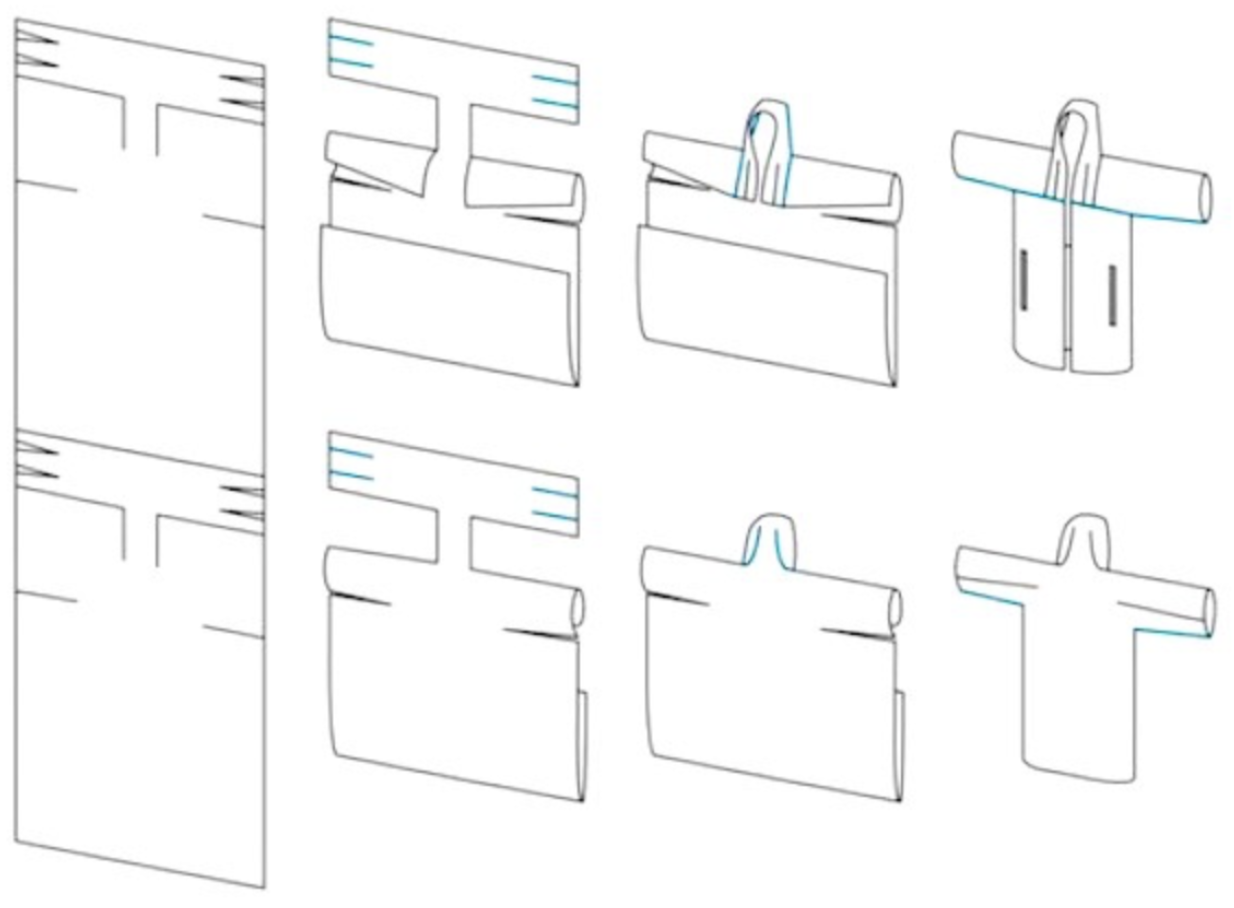
\includegraphics[width=\textwidth]{Images/rissanen jacket.png}
        \caption{Telfer duffle coat \cite{rissanen_zero-waste_2013}}
        \label{fig:rissanen_jacket}
    \end{subfigure}
    \hfill
    \begin{subfigure}[b]{0.4\textwidth}
        \centering
        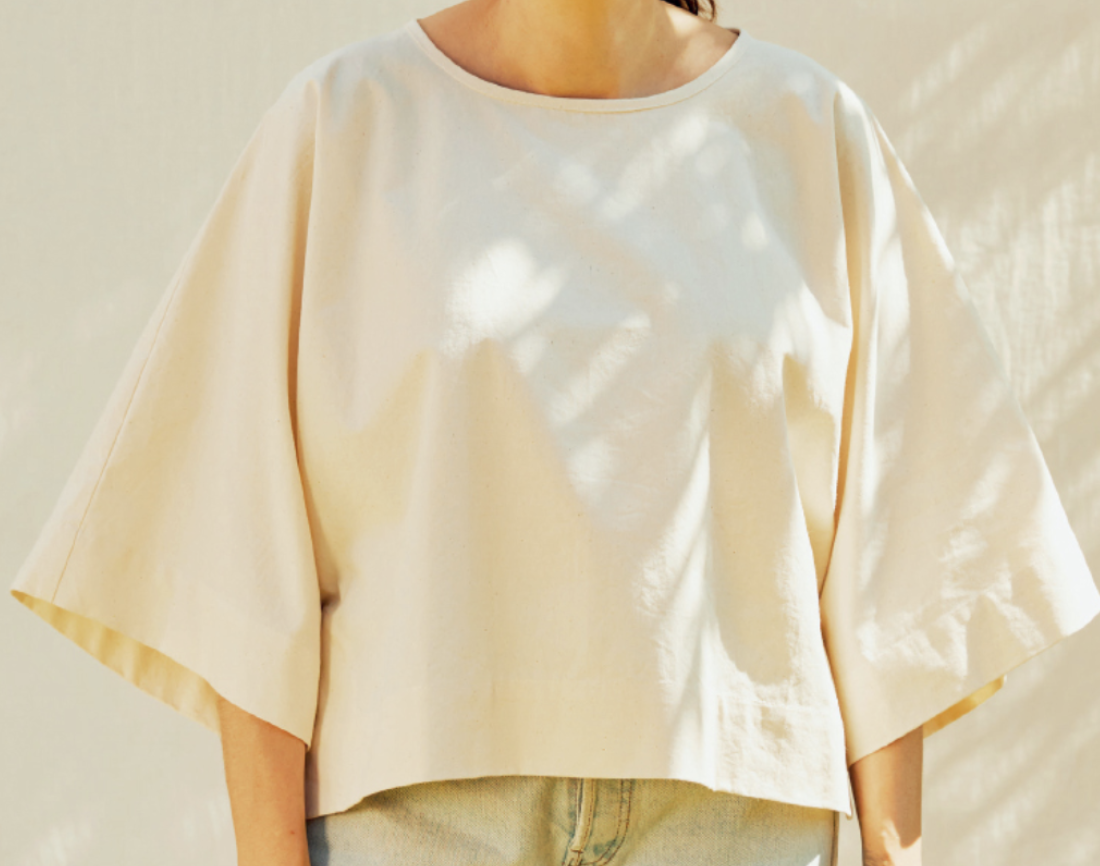
\includegraphics[width=\textwidth]{Images/bh tee.png}
        \caption{Helmersson Tee \cite{helmersson_zero_2023}}
        \label{fig:bh_tee}
    \end{subfigure}
    \caption{Examples showing boxy and loose-fitting aesthetic}
    \label{fig:jacket_tee}
\end{figure}

\section{Bespoke Clothing}
Fit and style are crucial factors for consumers when purchasing a garment. One-size approaches fail to accommmodate individual body variability. Achieving the right fit enhances satisfaction and extends the garment's life, reducing waste. Customisation adjusts a garment to an individual's physical dimensions, while personalisation reflects their unique style preferences. Together, they create bespoke clothing tailored to fit the individual's body and style, offering a sustainable alternative to mass-produced fashion .

Bespoke clothing also fosters a deeper connection between the garment and the wearer. Meticulous tailoring to personal measurements and style preferences increases the garment's significance, encouraging longer use and reducing the need for frequent replacements. This personalized approach contrasts with fast fashion's quick turnover and low cost, promoting more sustained use and lowering environmental impact.

The concept of a customised zero waste garment involves balancing fit and waste. Zero waste designs minimise fabric waste, while bespoke garments emphasize perfect fit and personalisation. Exploring this tradeoff is crucial for developing sustainable, personalised fashion solutions that reconcile zero waste design with bespoke tailoring, contributing to more environmentally friendly and consumer-focused garment production.

\section{Digitisation Trends in Fashion}
Digitization is revolutionising the fashion industry by transforming traditional methods of garment production and design with streamlined workflows. These technologies improve accuracy, efficiency, and sustainability, contributing to a more innovative and eco-friendly fashion industry.

\subsection{Body Scanning}
Body scanning technology provides precise measurements that enhance garment fit and customization. This technology utilizes 3D scanners to capture detailed body dimensions by emitting light or laser beams over the body surface and recording the reflected data. A digital model is creating from this data to represent the individual's shape and size. While precision of these measurements ensures consistency, accuracy can vary based on method and conditions. This technology is leveraged by retailers such  MTailor to offer custom-fit garments. Smartphones apps such as 3DLOOK provide a convenient way for consumers to scan themselves, though not to the precision of professional scanning machines.

\subsection{Digital Pattern Making}
Digital pattern making employs software to enhance the traditional by-hand pattern making process, making it more time and resource efficienct. Products like TUKAcad and Optitex allows designers to create and adjust patterns dynamically. This digitisation streamlines the pattern-making process, reducing errors and enhancing the production of bespoke clothing \cite{kim_garment_2003}.

AI patternmaking is still in its infancy as researchers estimate that effective implementation is \>5 away. Unlike digital patternmaking, AI faces two fundamental issues of reliability and controllability. It often requires numerous iterations to achieve acceptable results, and the outcomes are frequently unpredictable\footnote{Huamin Wang (STYLE3D), ``AI in Fashion Webinar," webinar, hosted by InnovateUK, April 19, 2024, https://iuk.ktn-uk.org/events/ai-in-fashion-webinar/}.

By integrating digital pattern making with body scanning, the fashion industry can achieve more precise and sustainable production methods, while AI continues to develop to further enhance these processes in the future.

\subsection{Digital Sampling}
Digital sampling enables designers to visualize and refine their creations before physical production. Software such as Marvelous Designer, Browzwear, and CLO 3D \cite{noauthor_2d_2024} allow the creation of detailed digital representations of garments, complete with realistic textures and draping effects on avatars. Virtual prototyping offers several advantages, including reduced time and cost associated with producing physical samples, and the ability to experiment with different styles and materials virtually.

These technologies enhance collaboration within the fashion industry by allowing designers, pattern makers, manufacturers, and consumers to share and review digital prototypes, ensuring the final product meets design specifications. Virtual showrooms and fashion shows are becoming more prevalent, offering brands a sustainable way to present collections globally without the environmental impact of physical events.

However, the challenges lie in fidelty. Digital samples are not as representative as physical samples. To achieve high fidelty, high labour cost and 3D modelling expertise is required.

\subsection{Exisiting Computational Frameworks}
Computational frameworks in fashion design integrate various tools and software, enhancing innovation and efficiency. Platforms like GarmentCAD and FashionCAD automate the pattern-making and grading process, using algorithms to ensure accurate fit across different sizes, improving productivity and reducing errors as shown in the examples below.

\subsubsection{Apparel Design Engineering (ADE) Group}
Gill et al. from the University of Manchester's ADE Group explore the concept of parametric blocks in their study on evolving pattern practice. They highlight the transition from traditional patterns to bespoke parametric blocks, which offer significant advantages in terms of customisability and sustainability. Parametric pattern construction involves defining parameters based on measurements and preferences that establish the relationship between pattern inputs and outputs, enabling dynamic and geometrically associative patterns \cite{gill_evolving_2023}. This method supports the creation of custom garments.

\subsubsection{Generative Garment Design for Circularity (GGD4C)}
Bigger's GGD4C proposes using generative algorithms to integrate lifecycle, material use, and circularity data at the garment design phase. This methodology shifts towards a more environmentally conscious fashion industry by incorporating circular design principles from the outset. The framework utilizes tools such as Grasshopper's evolutionary solver Galapagos in Rhinoceros 3D software to create parametric patterns optimized for material efficiency and circularity. Early experiments with GGD4C, such as the design of a jumpsuit, have demonstrated its potential to reduce environmental impact significantly. The generative approach allows for the simultaneous optimisation of multiple design objectives, aligning fashion design with sustainability goals \cite{bigger_generative_2021}.

\subsubsection{GarmentCode}
GarmentCode is a notable example of an advanced computational framework that applies object-oriented programming principles to garment construction. Its PyGarment library allows designers to create sewing patterns in a hierarchical, component-oriented manner. This approach enables the creation of complex, parametric garment designs that can be easily adjusted for different body measurements and styles. The system automates low-level tasks, such as placing darts, and supports the exploration of diverse design spaces. GarmentCode's configurator allows for the free manipulation of design parameters, enhancing creativity and efficiency in garment production \cite{korosteleva_garmentcode_2023}.
\begin{figure} [H]
    \centering
    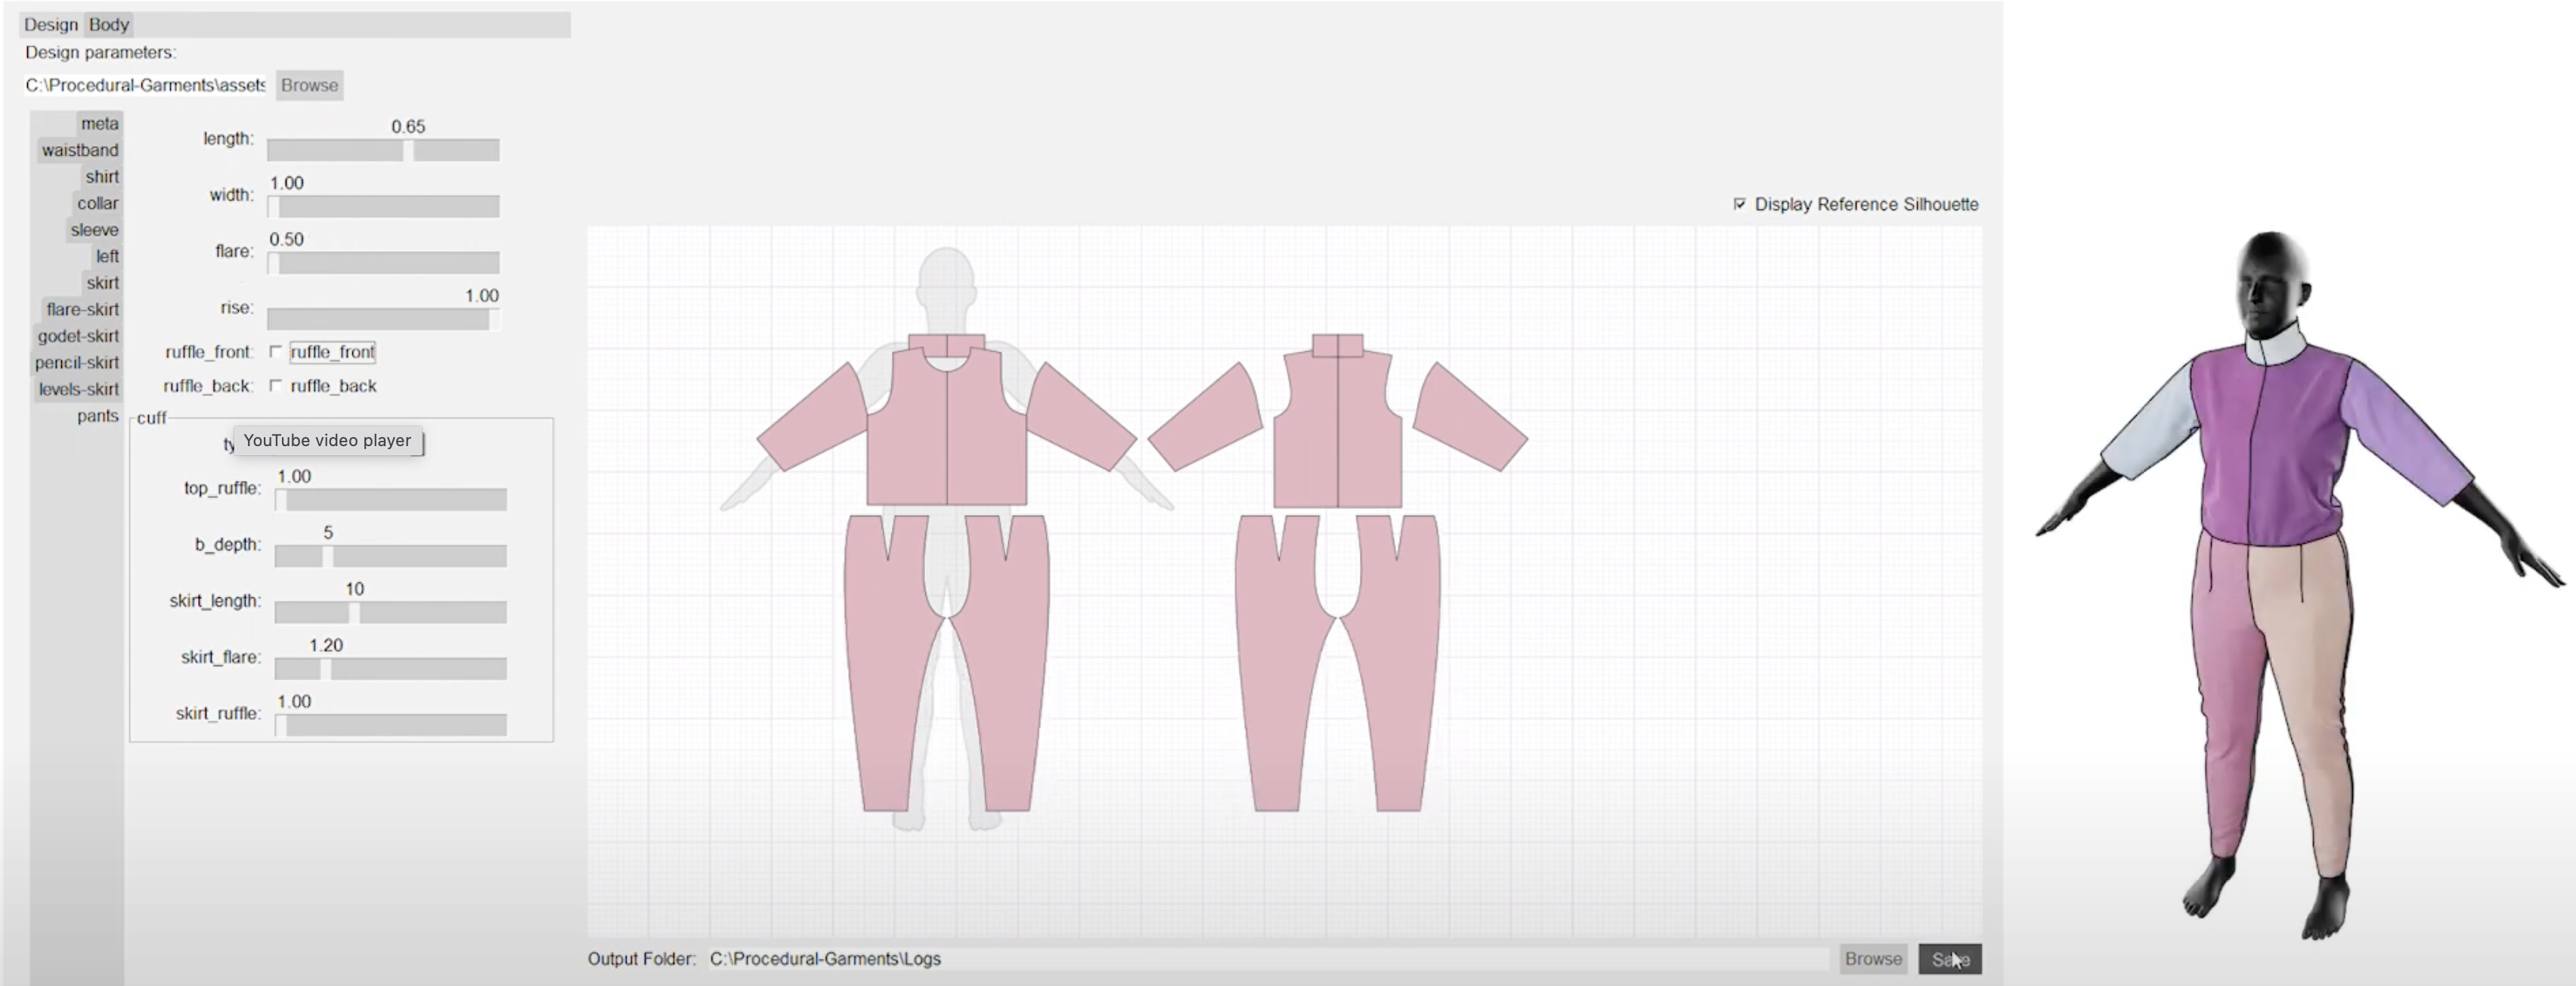
\includegraphics[width=0.8\textwidth]{Images/pygarment.png}
    \caption{Snapshot of GarmentCode GUI \cite{korosteleva_garmentcode_2023}}
\end{figure}

\section{Summary}
This review shows that traditional patternmaking results in fabric waste during production. Zero-waste patterns exist but are not easily parameterised given the complexity of their design. Bespoke clothing is valued by consumers. New digital tools exist that allow for easier body measurement, digital pattern making, and virtual prototyping. Computational frameworks make it possible to tie all these tools together and test on available datasets.

This project's novel contribution is to build a framework integrating these techniques to create bespoke parameterisation of an existing zero-waste pattern and provide efficiency metrics for the same.

\chapter{Design Engineering Process} 
\section{Research Aims and Goals}
\subsection{Context and Rationale}
This project addresses fabric waste in garment manufacturing by aiming to make zero-waste pattern making more accessible and inclusive. It seeks to resolve the lack of parameterisation methods for zero-waste patterns and the inability of current patterns to provide a good fit for diverse body types. Custom sizing for individuals enhances the garment's value to the wearer, but introducing a closer fit can lead to increased cut loss. Therefore, the project aims to parameterise a zero-waste pattern based on measurements and preferences, outline the waste impact, present methods to recoup cut loss through creative reuse for increased garment utility, and leverage 3D tools to provide visual representations before users commit to production.

\subsection{Scope}
This project targets the smaller-scale operations that can more readily adopt innovative and sustainable practices. It focuses on creating a single garment for an individual rather than addressing mass production.

One existing zero-waste pattern is selected for parameterisation. A new pattern design is not developed to reduce the project's scope of work. Furthermore, integrating of fabric properties and cost analysis are beyond the project's scope.

The aim is to create a framework enabling bespoke towards zero-waste pattern creation for both virtual modelling and physical production. The framework provides analytics on fabric use efficiency to suport informed decision-making. The project prioritises fit around the bodice over other areas of the body. Physical testing in a workshop study is used for evaluating the parameterisation method on fit qualitatively. Theoretical analysis on a publicly available dataset is used for evaluating the parameterisation method on fabric efficiency and cut loss quantitatively.

The author, a novice  fashion practice, applies design engineering methods to introduce novelty through zero-waste pattern parameterisation. Python is used for parameterisation, pattern file generation, and waste analysis. CLO 3D is used for virtual draping.

\subsection{Goals}
Key goals of the project include:
\begin{itemize}
    \item Develop a method that successfully takes in measurements and outputs a parameterised pattern for the garment.
    \item Calculate the ideal fabric bolt width for a given pattern's dimensions.
    \item Compute fabric efficiency and cut loss metrics based on user preferences for informed decision-making.
    \item Provide segmentation and reconstruction techniques to fit the pattern on available fabric bolt widths.
    \item Define and implement a strategy that repurposes cut loss to enhance the garment's utility and aesthetic appeal.
    \item Generate pattern files to visualise the garment on an avatar.
\end{itemize}

\section{Methodology}
Figure \ref{fig:tail0r pipeline} outlines the tail0r pipeline.

\begin{figure} [h]
    \centering
    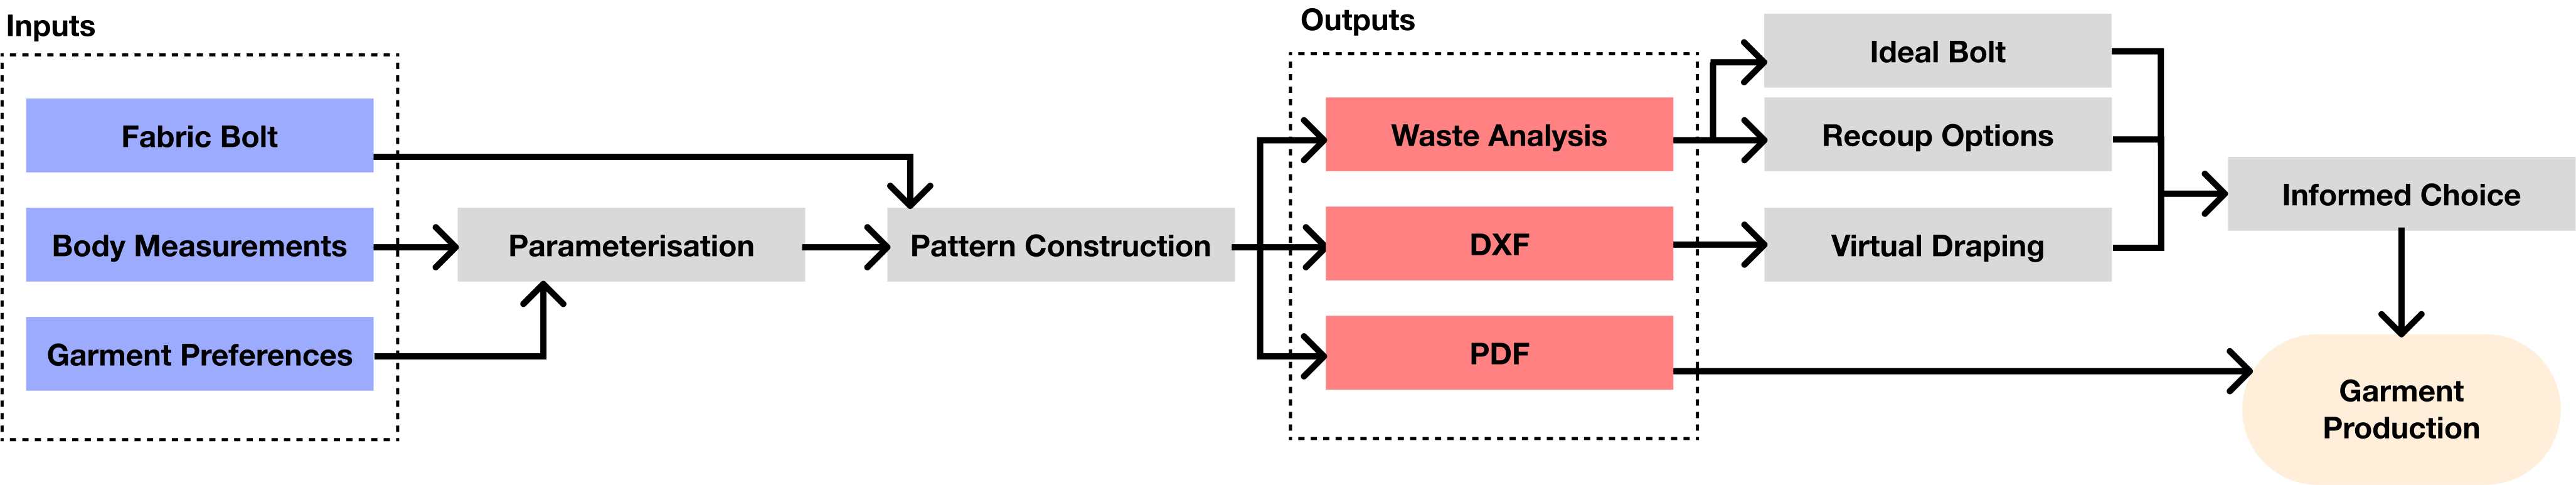
\includegraphics[width = \textwidth]{Images/tailor pipeline.png}
    \caption{tail0r Pipeline}
    \label{fig:tail0r pipeline}
\end{figure}

\subsection{Pattern Selection}
The chosen garment for this study is Helmersson's short-sleeved collared shirt with a back pleat and front button closure (Figure \ref{fig:bh shirt sketch}) from her book \textit{Zero Waste Patterns}. It's a ``one-size garment where the total body circumference [of the garment] is determined by the width of fabric'' used, forcing zero-waste. As a result, it's inherently loose-fitting and oversized, presenting a unique challenge in balancing zero-waste principles with a more tailored fit. She designates it as skill level 3 out of 5, being suitable for confident beginners. The garment was chosen for its relative simplicity in construction, symmetry of its pattern (Figure \ref{fig:bh shirt pattern}), and the challenge it presents in parameterising for a better fit.
\begin{figure} [H]
    \centering
    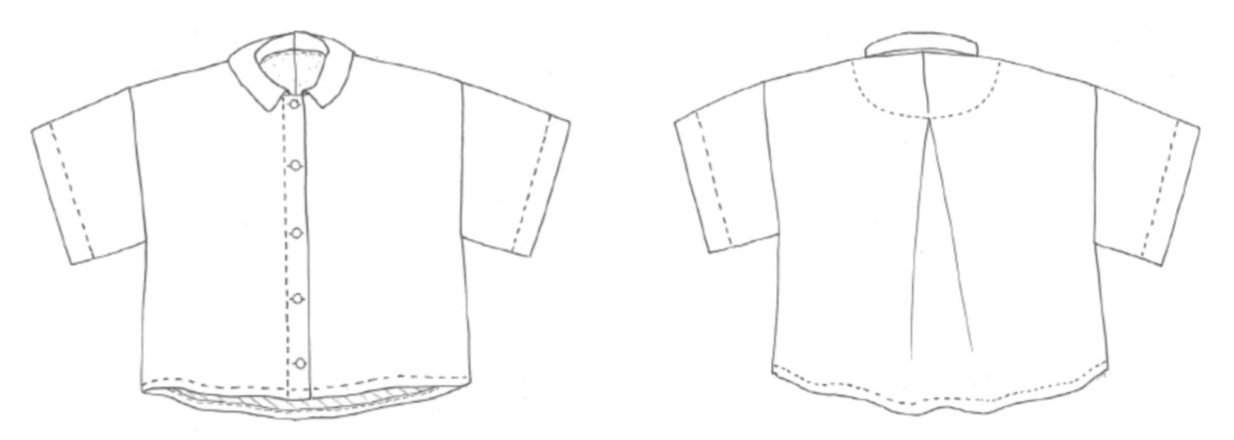
\includegraphics[width = \textwidth]{Images/finishedgarmentsilhoutte.png}
    \caption{Helmersson's Shirt sketch}
    \copyright {Birgitta Helmersson} % this prints the caption below the figure
    \label{fig:bh shirt sketch}
\end{figure}
\begin{figure} [H]
    \centering
    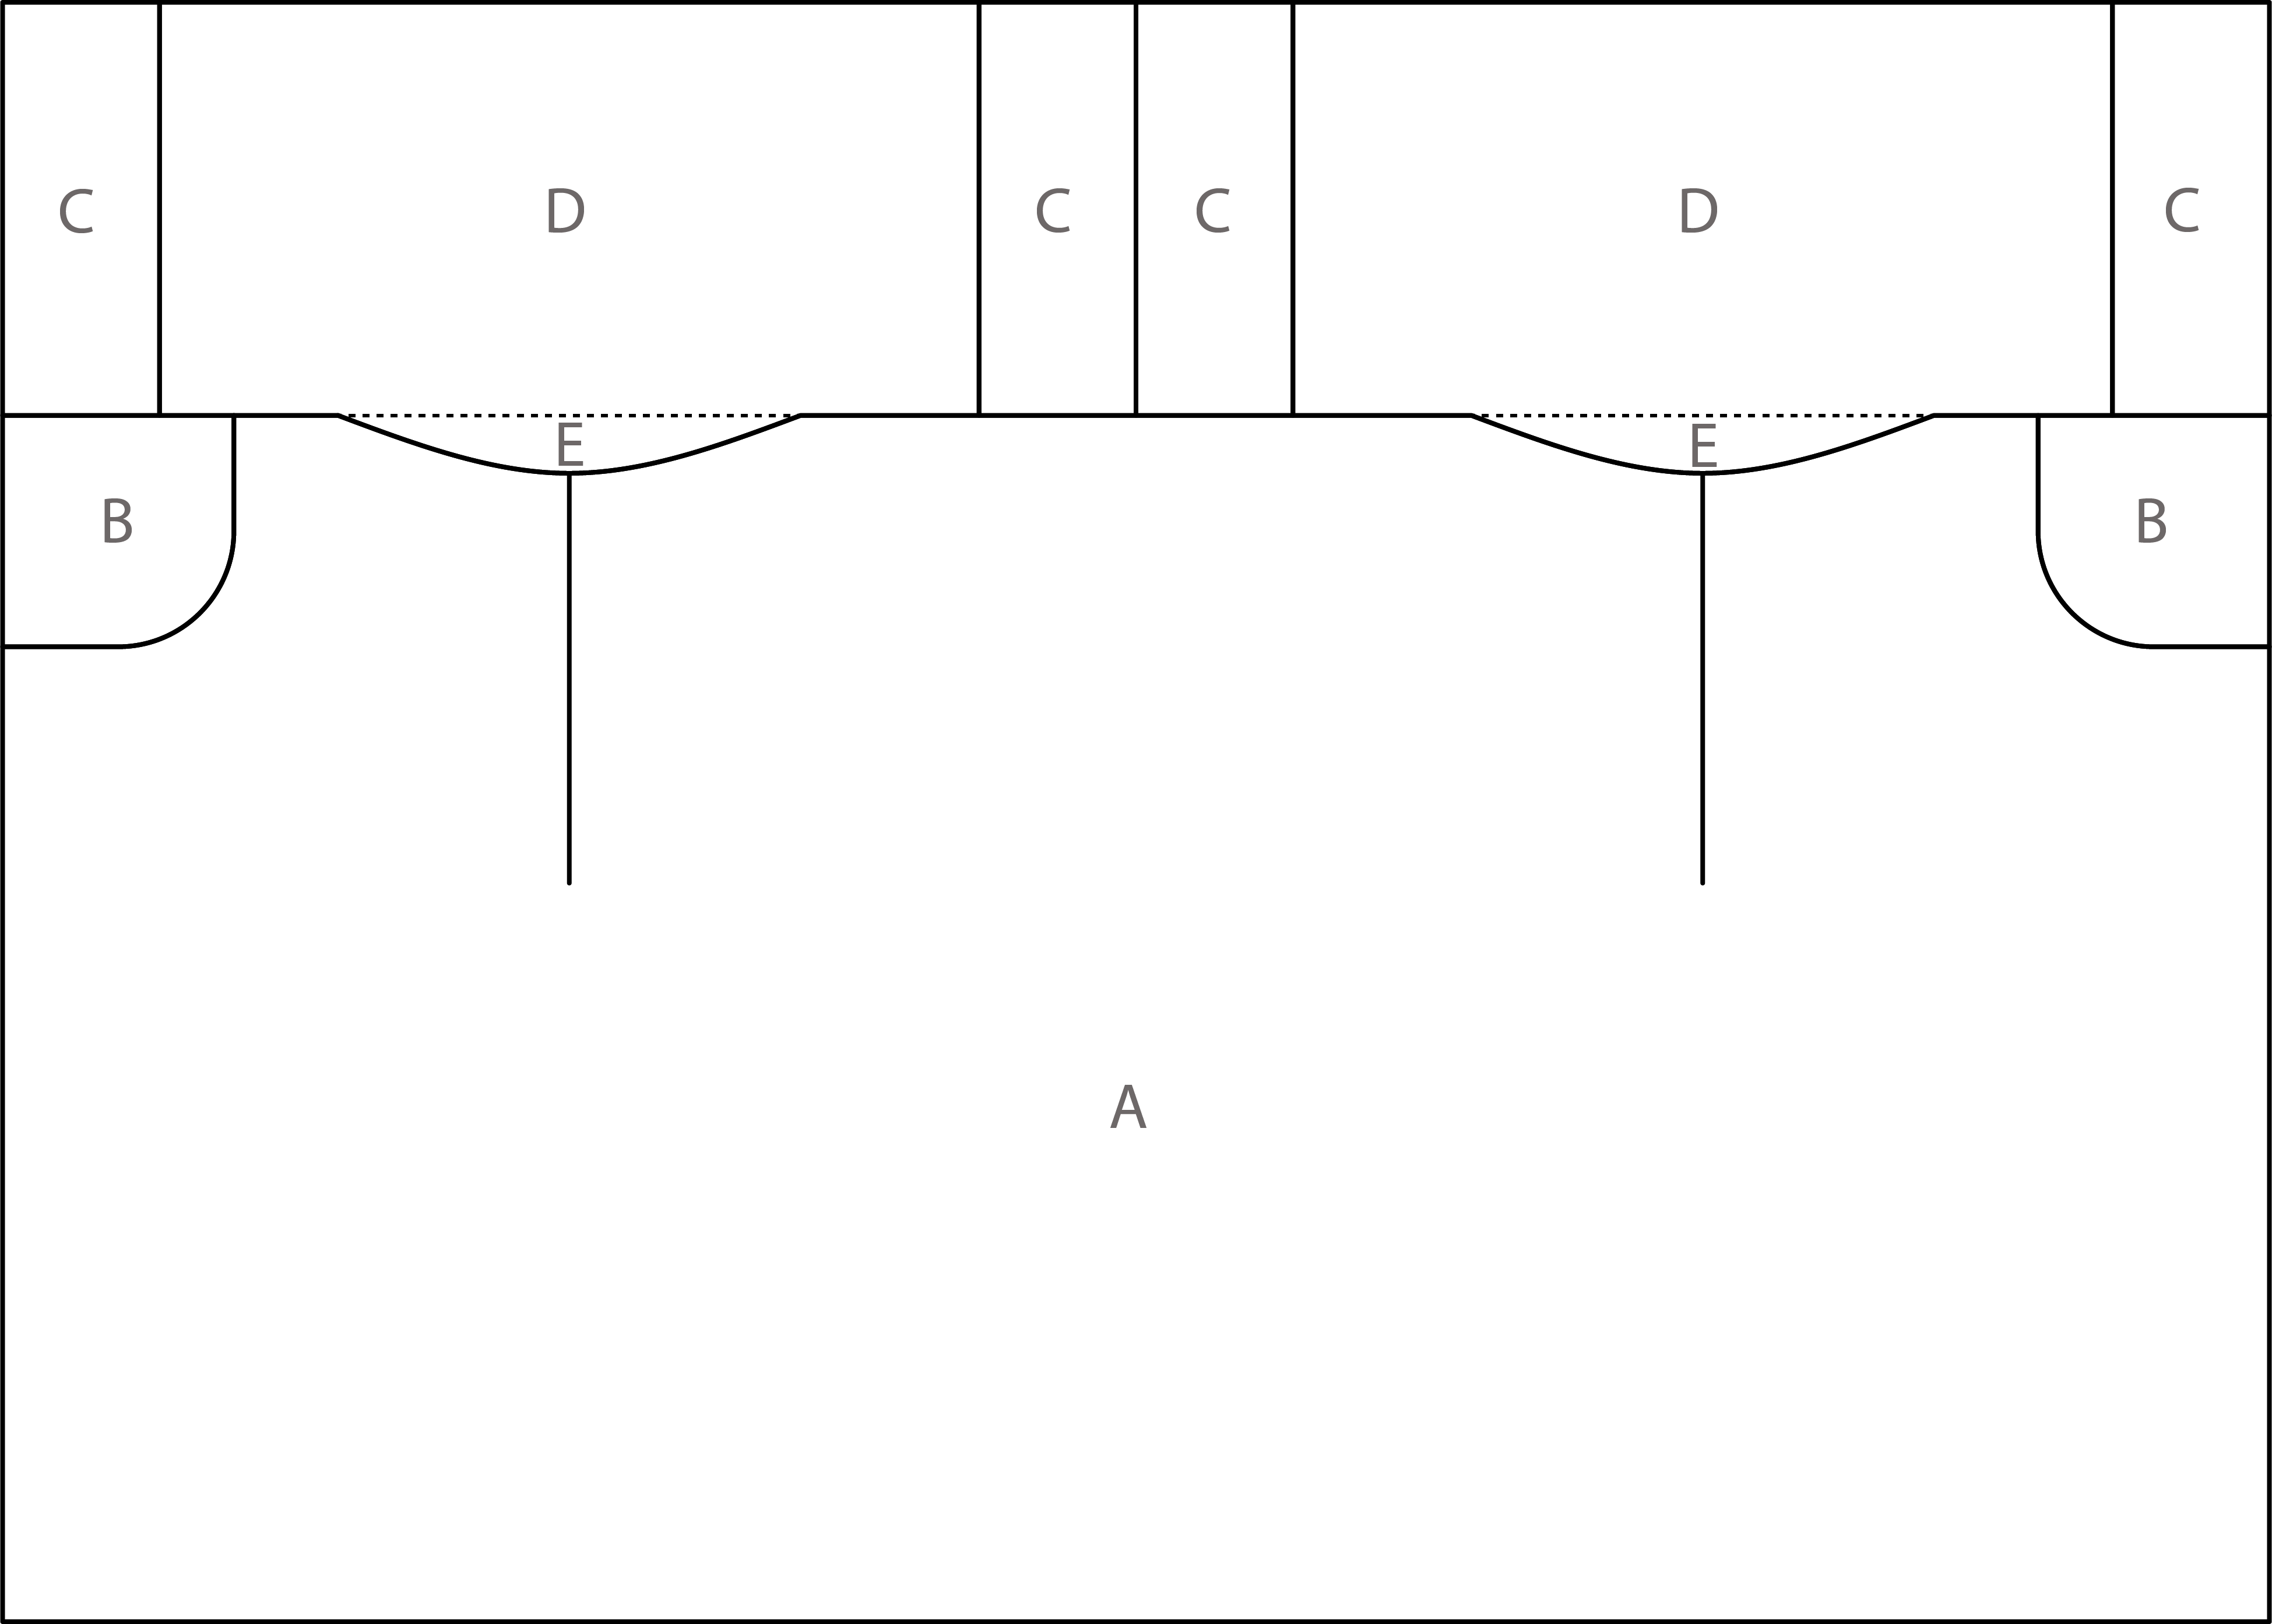
\includegraphics[width = 0.75\textwidth]{Images/originalpattern_whole.png} 
    \caption{Shirt block pattern}
    \label{fig:bh shirt pattern}
\end{figure}
\begin{itemize}
    \item \textbf{A} Front/back body piece
    \item \textbf{B} Back neck facing template
    \item \textbf{C} Collar pieces
    \item \textbf{D} Sleeve pieces
    \item \textbf{E} Sleevehead curve template
\end{itemize}
Helmersson's method does not require large paper patterns; instead, designs are drawn directly onto the fabric and cut. For constant pieces, she provides small printable templates, maintaining fixed sizes for B, C, and E. Her sizing chart (Figure \ref{fig:bh size chart}) includes about 25 cm of ease, combining both wearing and design ease. This ease is applied generally, not to individual areas. The chart only considers fabric widths within a 20 cm range and bases sizing only on chest/bust and hip measurements, with fabric with being 31 cm greater than the largest max circumference. This includes 25 cm of ease and 6 cm seam allowance, values used for parameterisation.
\begin{figure} [H]
    \centering
    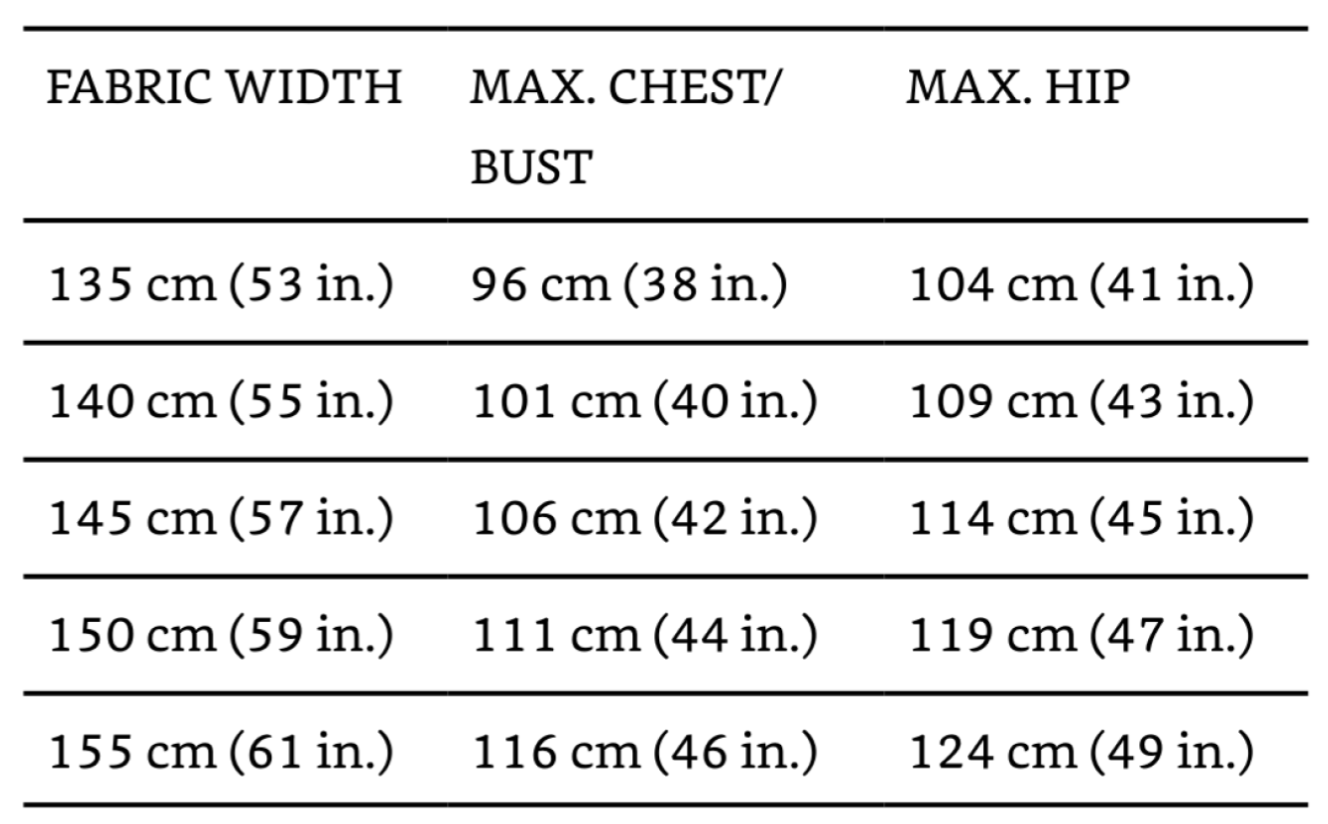
\includegraphics[width = 0.5\textwidth]{Images/BH size chart.png} 
    \caption{Helmersson's Shirt sizing chart}
    \copyright {Birgitta Helmersson}
    \label{fig:bh size chart}
\end{figure}
Notions (bindings, buttons, iron on interfacings, etc.) are not considered. These are components of the final garment not sourced from the original rectangle cut from the fabric bolt, therefore, are not part of the waste analysis.

%%%%%%%%%%%%%%%%%%%%%%%%
% PATTERN PARAMETERISATION
%%%%%%%%%%%%%%%%%%%%%%%%

\subsection{Pattern Parameterisation}
Now that the original garment type is understood, we can dissect the pattern into individual segments for parameterisation.
\begin{figure} [H] 
    \centering 
    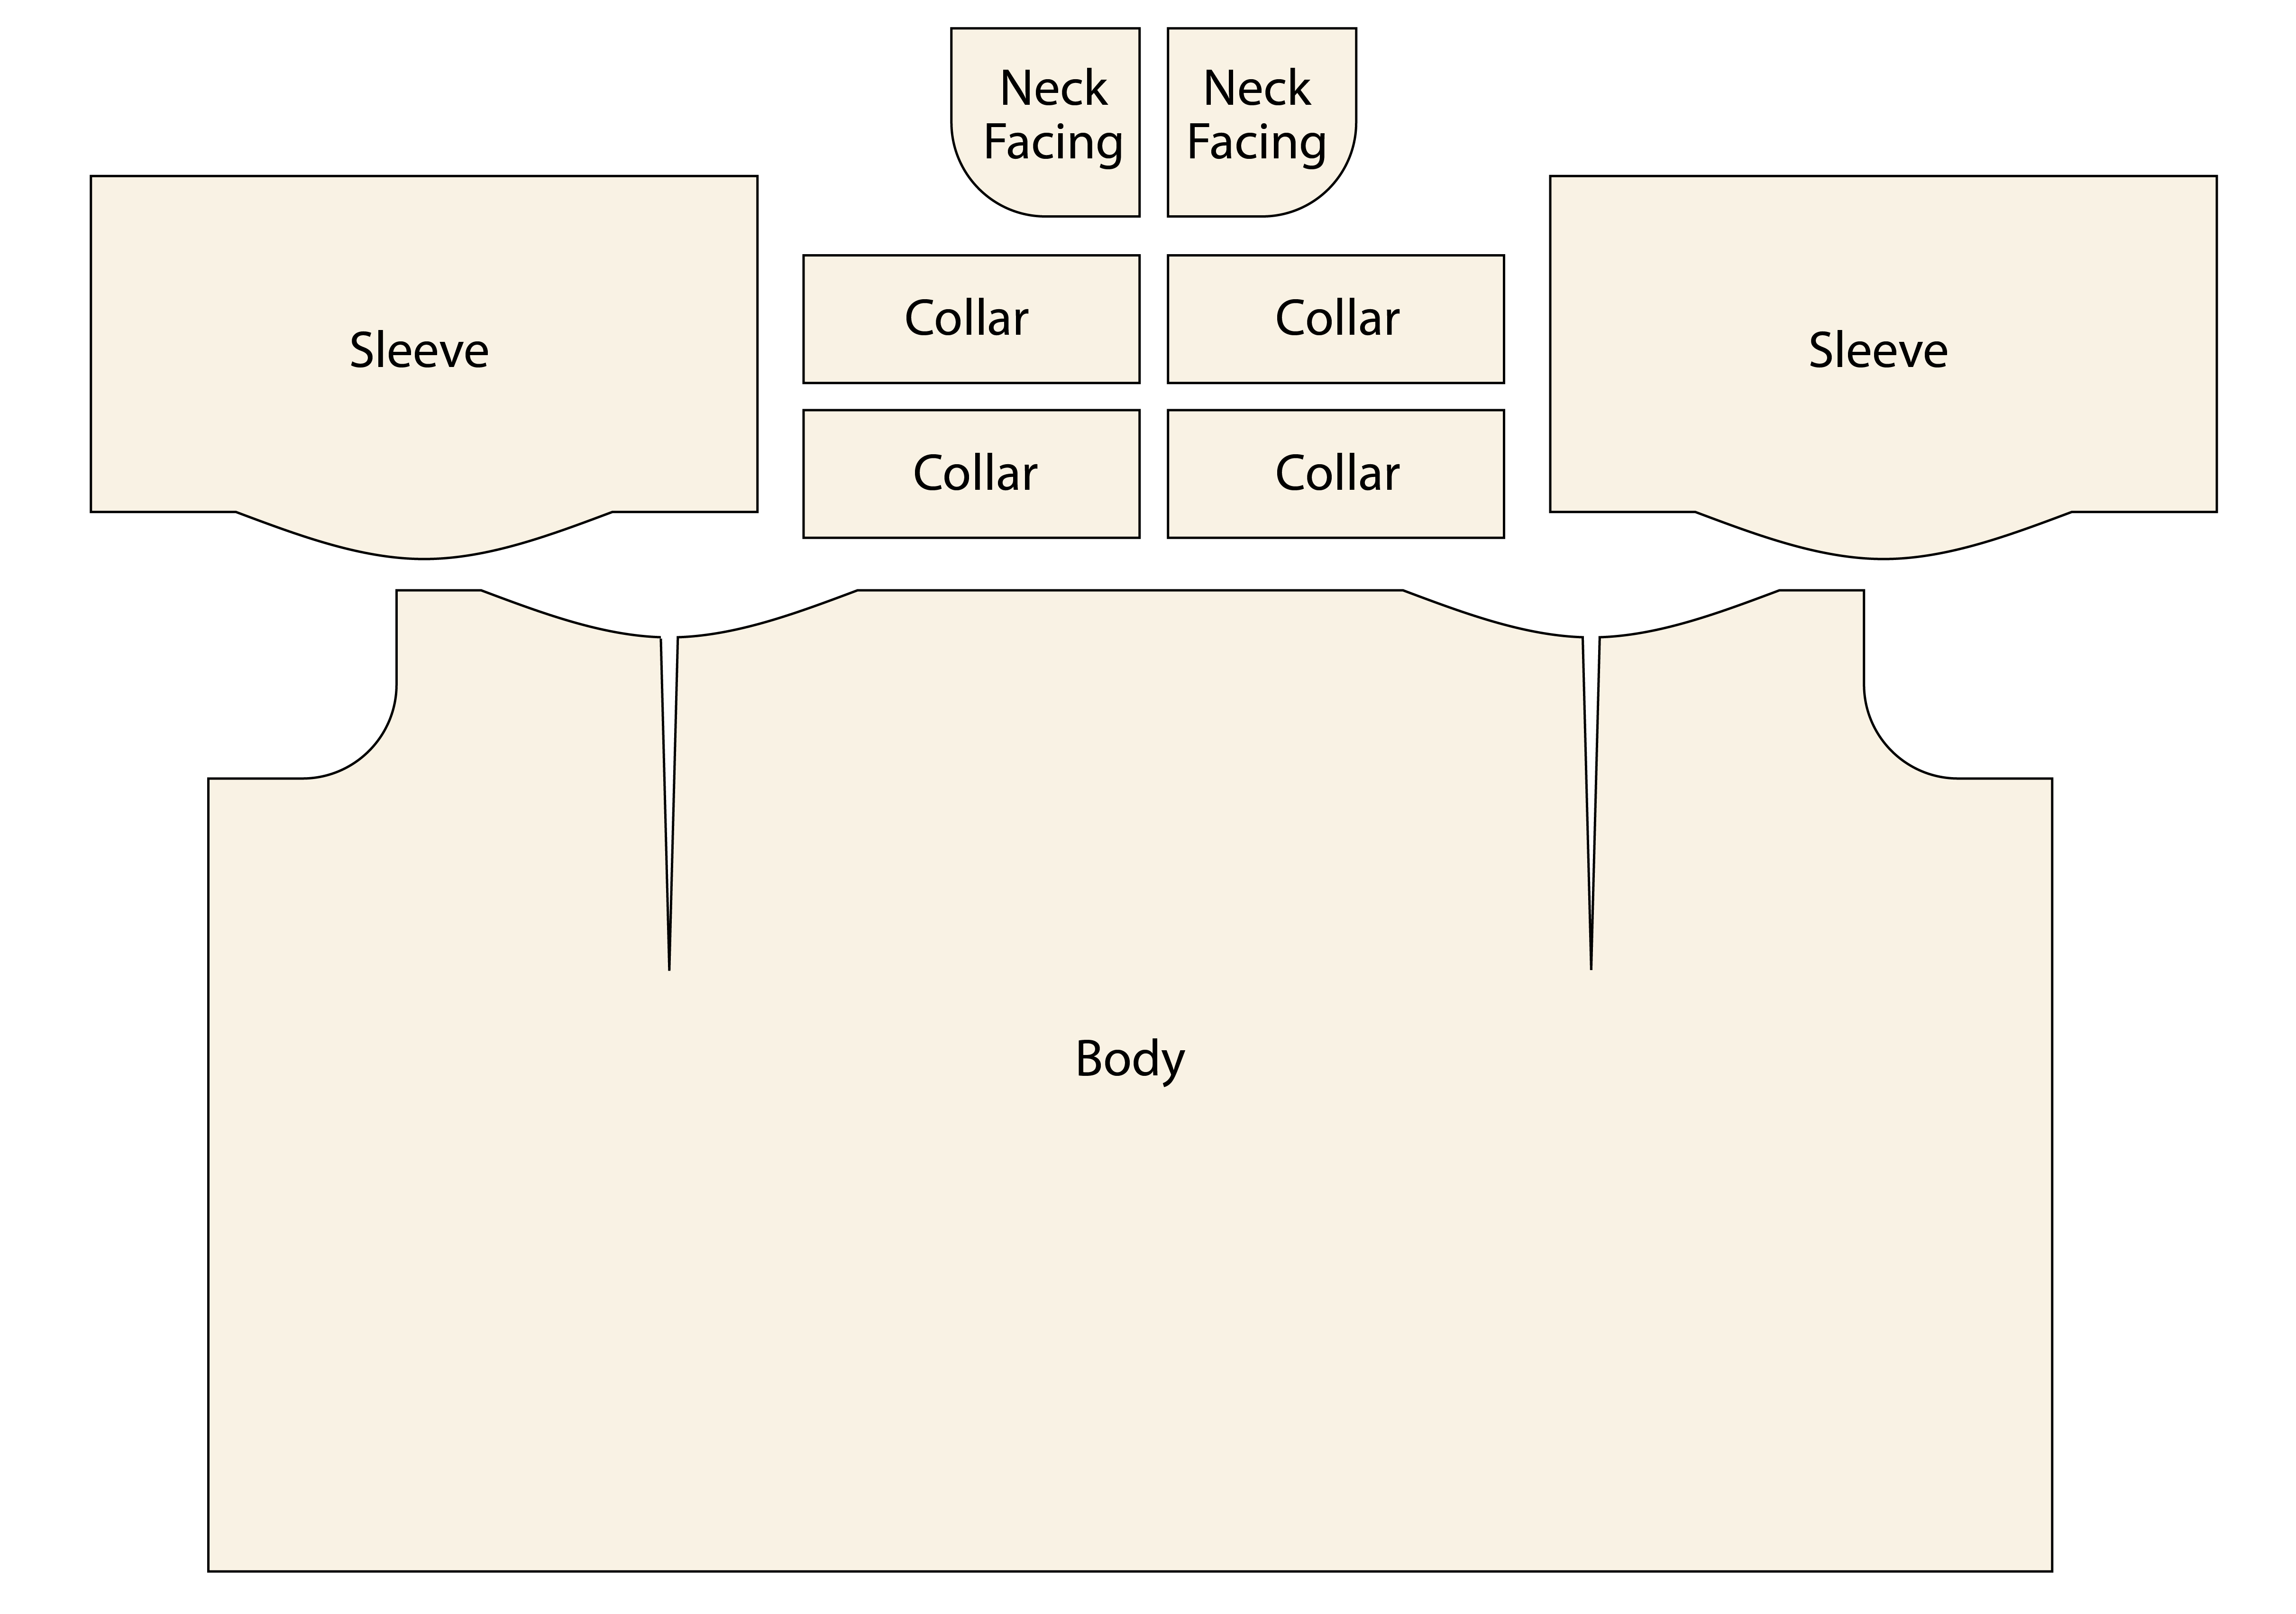
\includegraphics[width = \textwidth]{Images/originalpattern_pieces.png} 
    \caption{Shirt block pattern pieces}
\end{figure}
There are a total of nine (1x body, 2x neck facing, 4x collar, 2x sleeve) pieces that make up the block. Note that D and E combine to form the sleeve piece. There are no side seams on the shirt as there is just a single body piece, not a separate front and back.

\begin{table} [H] % this tells the compiler that a table environment is starting
    \centering % this puts it in the horizontal centre of the page
    %\rowcolors{1}{}{Gray} % this sets up the alternating grey/white background
    \begin{tabular}{p{2cm}|p{5cm}} % this sets up the tabular environment ant states the width of the columns, you could use an equation here using the \textwidth, but i have no experience with this. 
    
        %the following lines populate the table with data. They follow the pattern
        % item & item & item & item \\
        % where the ampersand denotes a vertical line, and the double slash, a new line.
        \textbf{Shortform} & \textbf{Parameter}\\
        \hline % this produces a horizontal line, this could be used elsewhere in the table
        pw& pattern width\\
        ph& pattern height\\
        cw& collar piece width\\
        ch& collar piece height\\
        bw& neck facing width\\
        bh& neck facing height\\
        sd& sleevehead curve depth\\
        sr& sleevehead curve radius\\
        al& armhole length
        \end{tabular}
    \caption{Pattern Parameters Table}
\end{table}
\begin{figure} [h] % opens the figure environment. the '[H]' forces the image to be Here
    \centering % puts the image in the horizontal centre of the page
    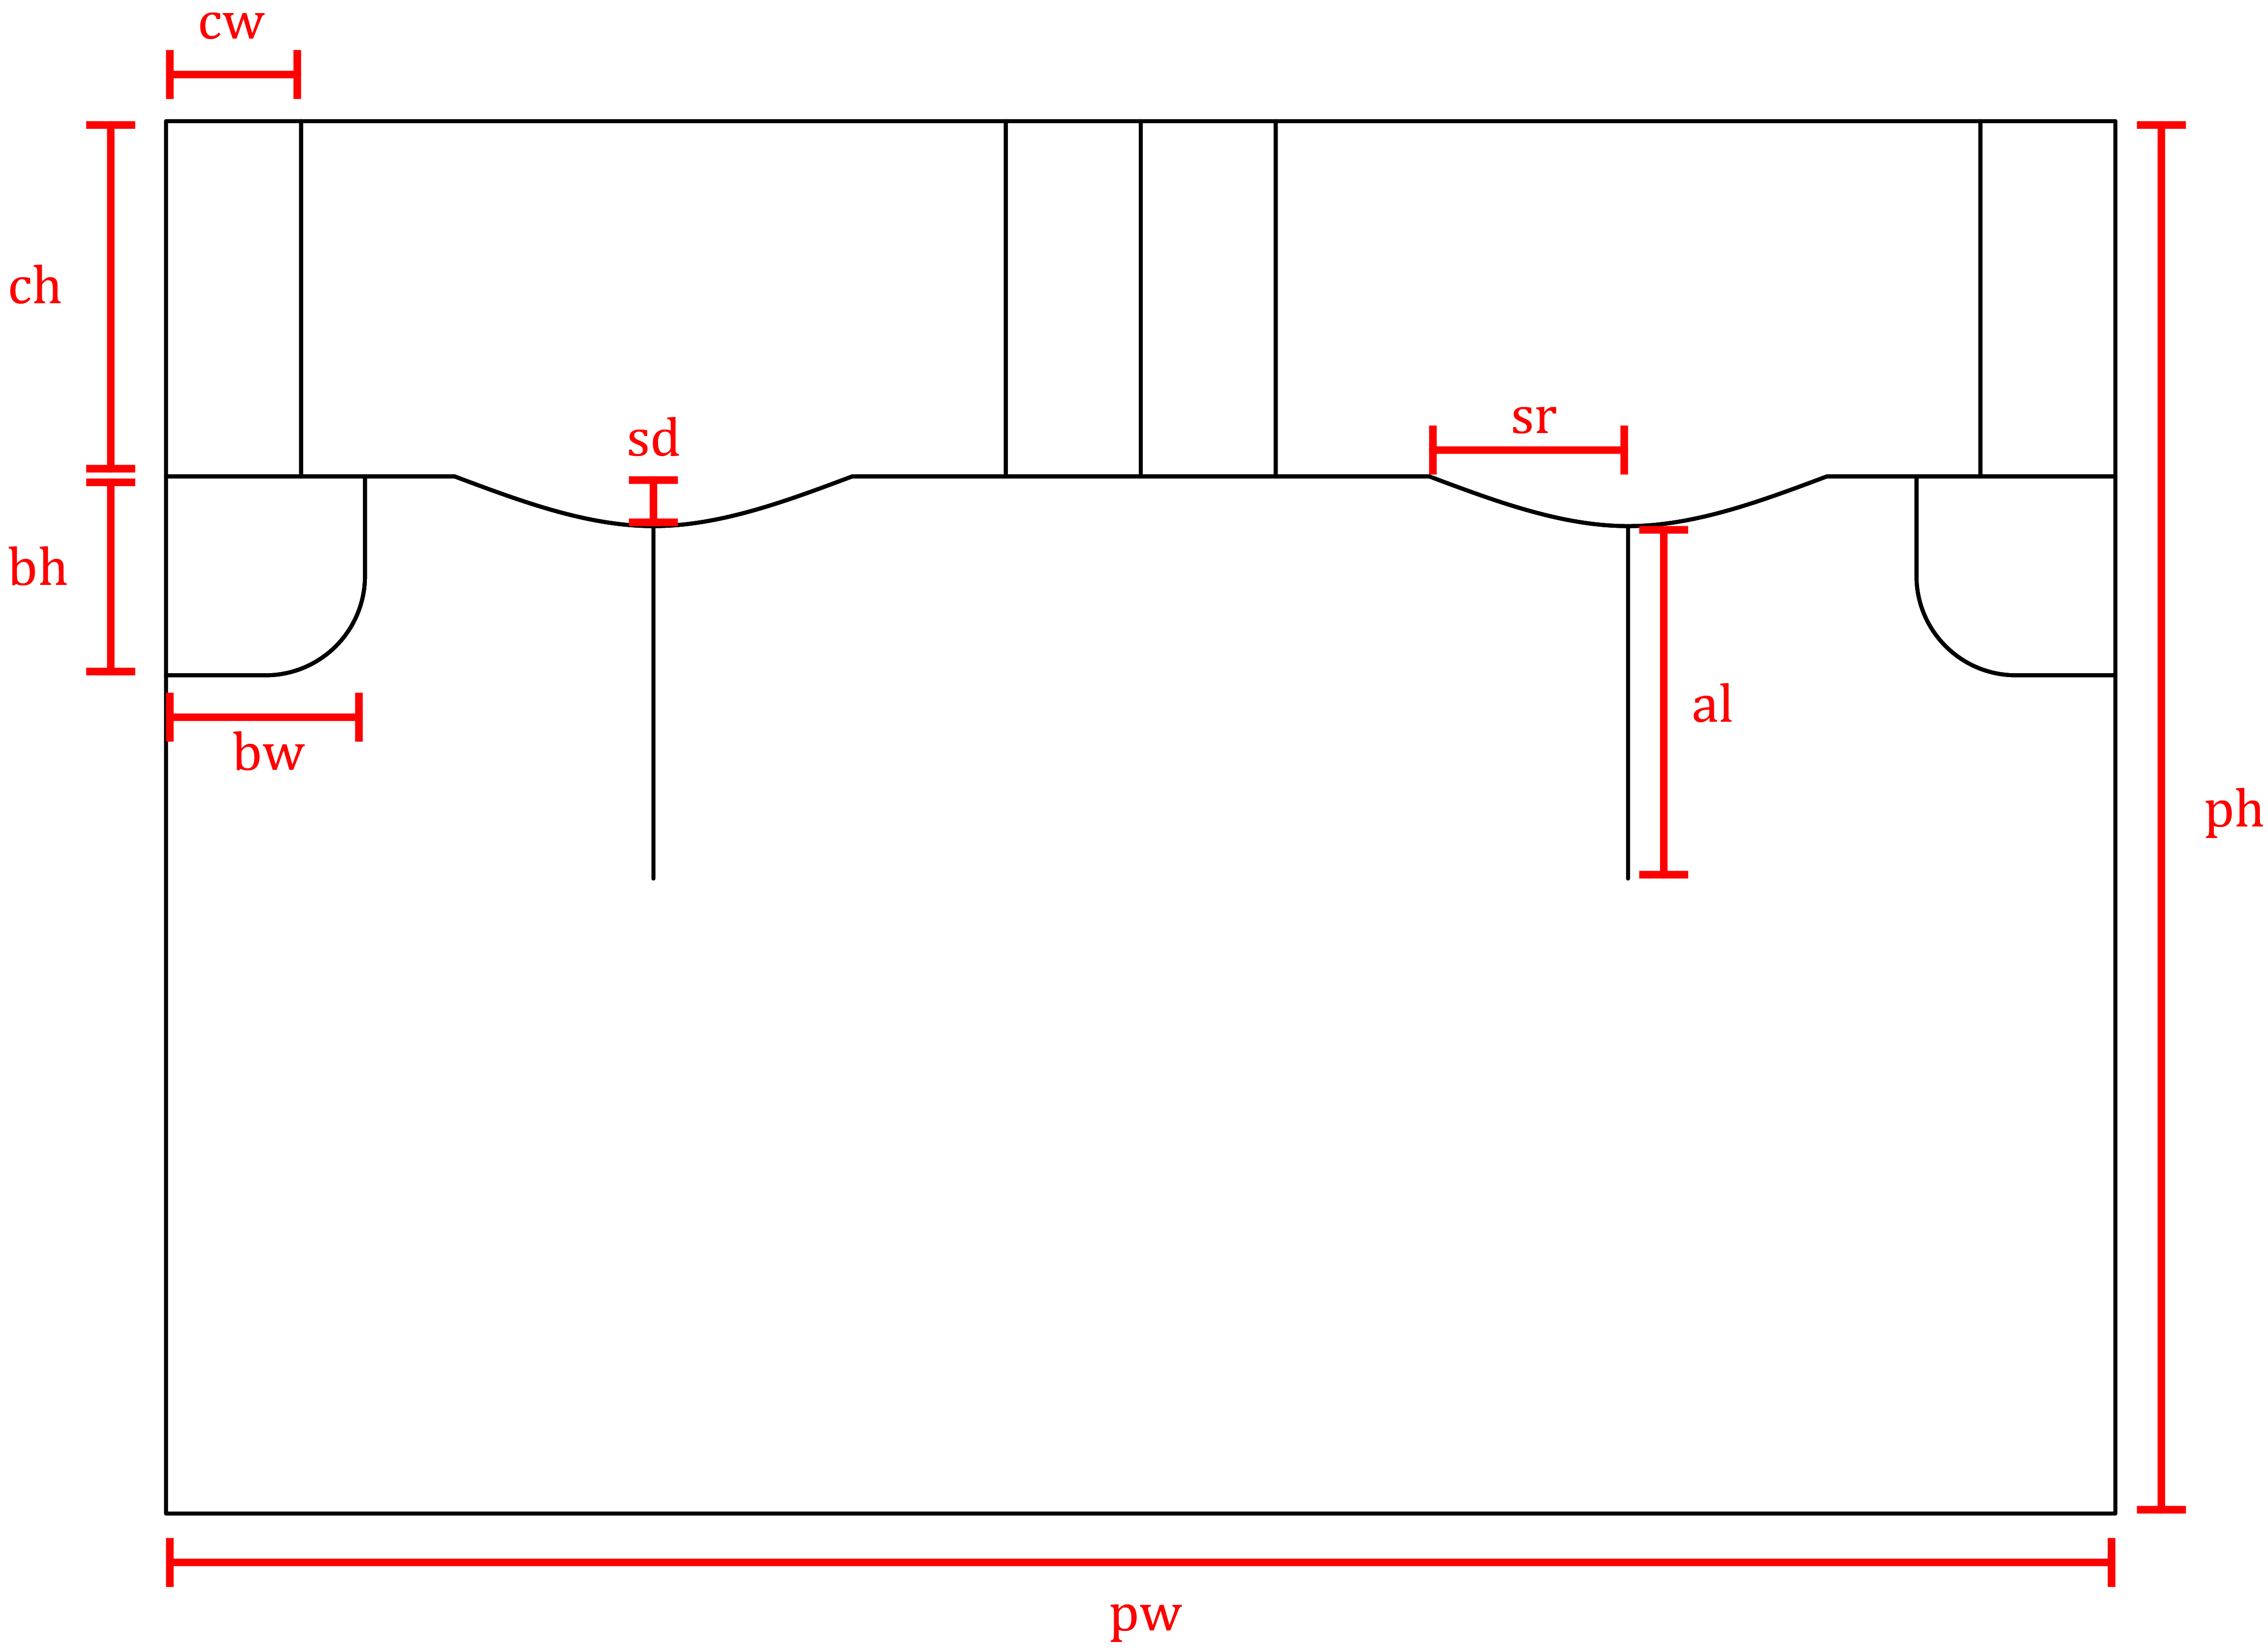
\includegraphics[width = \textwidth]{Images/pattern params.png} %this tells latex what graphics to include. I put my images in an 'Images' folder to aid file management, hence the Images/ before the file name. the width bit before allows you to alter the width of the image. It is also possible to use scale as well as using equations with the textwidth to make it say half the text width.
    \caption{Pattern Parameters Diagram}
\end{figure}

The process for parameterising was based on traditional measurements professionals use for a tailored shirt. How these measurements can translate into algorithm for the pattern parameterisation was investigated.

By looking at the pattern, we quickly realise that scaling one dimension has an effect in multiple pieces. For example, increasing the pattern width will also enlarge the sleeve pieces. Therefore, it requires some nuance and compromise to be able to scale pieces effectively while still keeping the rectangular nature of the overall pattern. We are primarily concerned with calculating the pattern width and pattern height as these define the pattern at large. We are less focused on the definition of each piece's dimensions at input because some of these factors will be deduced by the pattern width and pattern height along with the layout of the pieces given the fabric bolt used to make the garment.

The fit around the bodice is the primary factor to be customised. Given this, the process starts by defining what will be kept constant. The collar piece is kept constant inline with Helmersson's dimension suggestions with collar piece width of 9.5 cm and collar piece height of 25 cm. It becomes clear that a segment is shared between the collar piece (C) and the sleeve piece (D). Collar piece height corresponds to the sleeve length measured from the shoulder point to the sleeve end(barring any hemming for now). The first relationship between pattern and finished garment discovered is that the sleeve length equals the collar piece height, 25 cm in this case.

The placement of the notches used to determine the finished pleat size and the button placket are also kept constant for everyone. For now, the general ease of the garment will also be constant with Helmersson's suggestion of 25 cm. 

The collar piece height also influences the overall pattern height. The height of the body piece (A) plus the collar piece height equals the total pattern height. From the center back linein the pattern, it is evident that the height of the body piece can be related to the shirt length measured from the center back base of the neck to the finished hem at the bottom. Shirt length is a personal choice and not a strict body measurement based input. The garment will employ a standard shirt 2.5 cm hem at the bottom for a clean finished. This hem allowance must be considered as it will come from the original fabric piece in maintaining zero waste design.
\begin{equation}
    \mathrm{pattern\ height} = \mathrm{desired\ shirt\ length} + \mathrm{collar\ piece\ height} + \mathrm{hem\ allowance}
    \label{eq:pattern height}
\end{equation}

with shortform and constants,

$ph = desired shirt length + ch + hem allowance$

if shirt length is 65 cm 

$ph = desired shirt length + 25 + 2.5$

The parameterisation assumes the pattern with will be equal to the largest circumference of the bodice plus the general ease and sew allowance for the body. We still intend to keep the aesthetic of the garment while provide fit to extend garment utility in terms of more wear time/uses.
\begin{equation}
    \mathrm{pattern\ width} = \mathrm{largest\ bodice\ circumference} + \mathrm{general\ ease} + \mathrm{sew\ allowance}
    \label{eq:pattern width}
\end{equation}

with short and constants,

$pw = largest bodice circumference + 25 + 6$

From the pattern, it is clear that scaling pattern width had an effect on the sleeve pieces. The collar piece widths (cw) are kept constant. By looking at the top border of the pattern, we see that pattern width also equals four collar piece widths plus two (one for each sleeve piece) top edge segments of the of the sleeve.

pw = 4*cw + 2*(sleeve top edge)

therefore

sleeve top edge = (pw - 4*cw) / 2

The sleeve top edge represented the sleeve circumference. Therefore, scaling up the pattern width will also scale up the sleeve circumference i.e. larger bodies will have baggier sleeves.
The armhole length (al) is equal to half of the sleeve top edge. This is because when the sleeve is sewed it needs to fit in the armhole with is formed when cutting the armhole length at the middle of the sleevehead curve and sewing the shoulder seams.

al = (pw - 4*cw) / 4

What is left is deciding how to scale the template sizes. Starting from her pattern as inspiration, we are simplifying the pattern even further to use simpler shapes when constructing these templates. Based on her size chart we are identifying an "ideal" largest circumference range for this pattern based on her chart and using her expertise as a fashion designer. This ideal range for the pattern then is 95cm to 125cm. We will use this ideal range to determine if a person gets the standard template size. People below this range will get slight smaller template size and people above this range will get bigger template size. Helmersson claims that beyond 25 cm of these measurements then the pattern might not be suited for you, we are aiming to make it more inclusive and account for other custom sizes with our parameterisation. 

For the standard neck facing template (B) size, We use square and circle inscribed in that square for the simple shape. Remember that these pieces help form the button placket, front neck line, and the overall pieces for the back neck facing. The facing piece height and width equal each other at 14 cm.

bw = bh = 14 cm

The facing piece curve horizontal line segment and facing piece curve vertical line segment are equal to each other and also equal to half of the facing piece width.

bx = by = (bw/2) = 14/2 = 7 cm

This 7 cm will also be the radius of the circle used to form the curve corner of the piece. So it is a quarter circle with radius of 7 cm forming and its end joins with the ends of horizontal and vertical line segments of the piece.

For the sleevehead curve template (E), an approximated and simplified verson of BH's template is using a sleevehead curve radius of 14cm and and sleevehead curve depth of 3.5cm. Notice that the sleevehead curve radius and facing piece width/height are the same. We keep this same relationship for deciding the other two template sizes.

For below 95 cm largest circ, we decrease the template size of facing piece width and height as 12 cm, sleevehead curve radius at 12 cm, and sleevehead curve depth at 3.0cm.
For above 125 cm largest circ, we increase the template size of facing piece width and height as 16 cm, sleevehead curve radius at 16 cm, and sleevehead curve depth at 4.0cm.
So it is a ±2 cm for the B5 piece width/height and sleevehead curve radius, and a ±0.5cm for the sleevehead curve depth.

The sleevehead curve depth influences the point where the sleeve attaches to the body at the shoulder point. We need to consider appropriate scaling of neck facing and sleevehead curve template because it affects the shoulder seam lengths. If these were always kept constant, it is possible that for smaller pattern widths it will eat into the top shoulder seams length and not fit the person because it is too small. This is a point we need to test for and do in the workshop. We will test if we are being too aggressive with this or not and if there are any not as obvious consequences.

The shapes were simplified not only to make recreating the pattern easier and more standardized but also for ease of use when constructing the pattern in DXF file format. The simple shapes help to streamline and ensure lines were meet at shared points, essential for ensuring the closed shape. 

%%%%%%%%%%%%%%%%%%%%%%%%
% FRAMEWORK OUTPUTS
%%%%%%%%%%%%%%%%%%%%%%%%

\subsection{tail0r Outputs}
The program creates the following outputs:
\begin{enumerate}
    \item A choice of patterns based on user's fit, style, and waste choices.
    \item Fabric usage efficiency metrics using ideal and given bolt widths for pattern choice.
    \item Embellishment strategies and applications for both.
    \item The DXF file that can be loaded into the CLO application for virtual draping and visual fit cues.
    \item The PDF file with return pattern measurements and annotated pattern image with dimensions that allows user to draw pattern on fabric and cut it out pattern.
\end{enumerate}

\subsubsection{DXF Pattern File}
The DXF file format is a standard of digital garment patterns. This format can be imported into many different pattern and 3D fashion applications including CLO 3D. The `ezdxf’ Python library \cite{noauthor_spline_nodate} was used for creating the DXF files of the pattern. Line, spline, lightweight polyline, and arc primitives were built into base functions to map out the geometry. The accompanying `ezdxf viewer’ was used for output verification.

Each pattern piece created via DXF needs to be a closed shape for successful import (Figure \ref{fig:successful import}). Pieces that share borders need to have their own representation of the shared segment and thus had to be redrawn as needed for the number of pieces they help define. This was achieved by defining layers (Figure \ref{fig:layer toggle}) for each piece type within the document modelspace. Figure \ref{fig:example dxfs} shows examples of the DXF pattern outputs.

\begin{figure} [H]
    \centering
    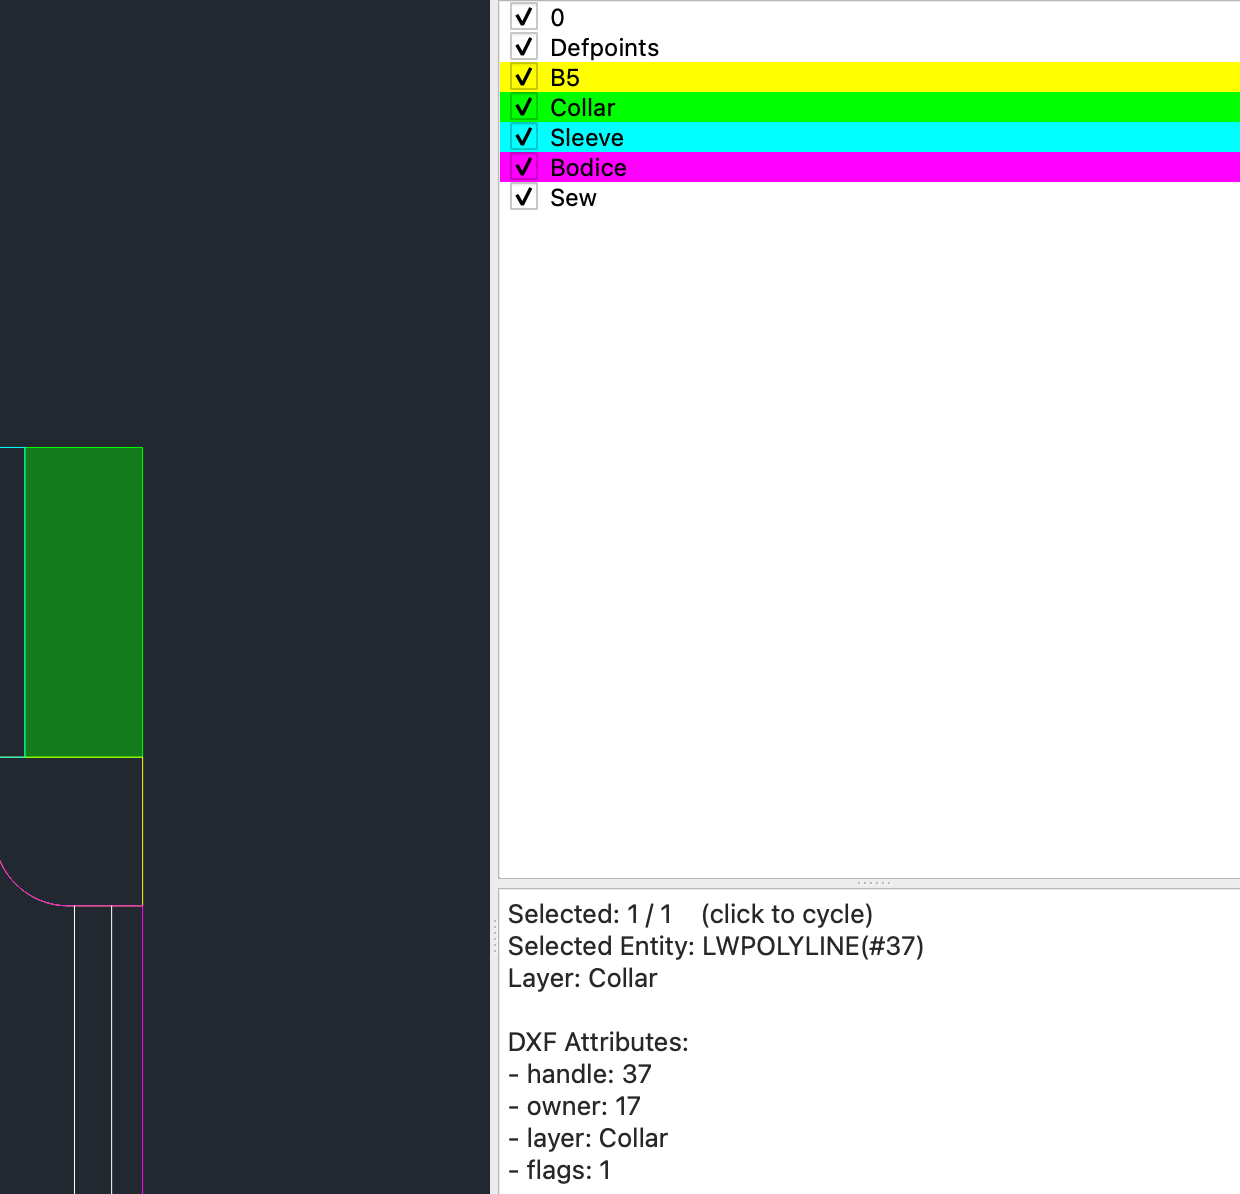
\includegraphics[width = 0.4\textwidth]{Images/dxf viewer.png}
    \caption{Layer toggle feature in ezdxf viewer}
    \label{fig:layer toggle}
\end{figure}

\begin{figure} [H]
    \centering
    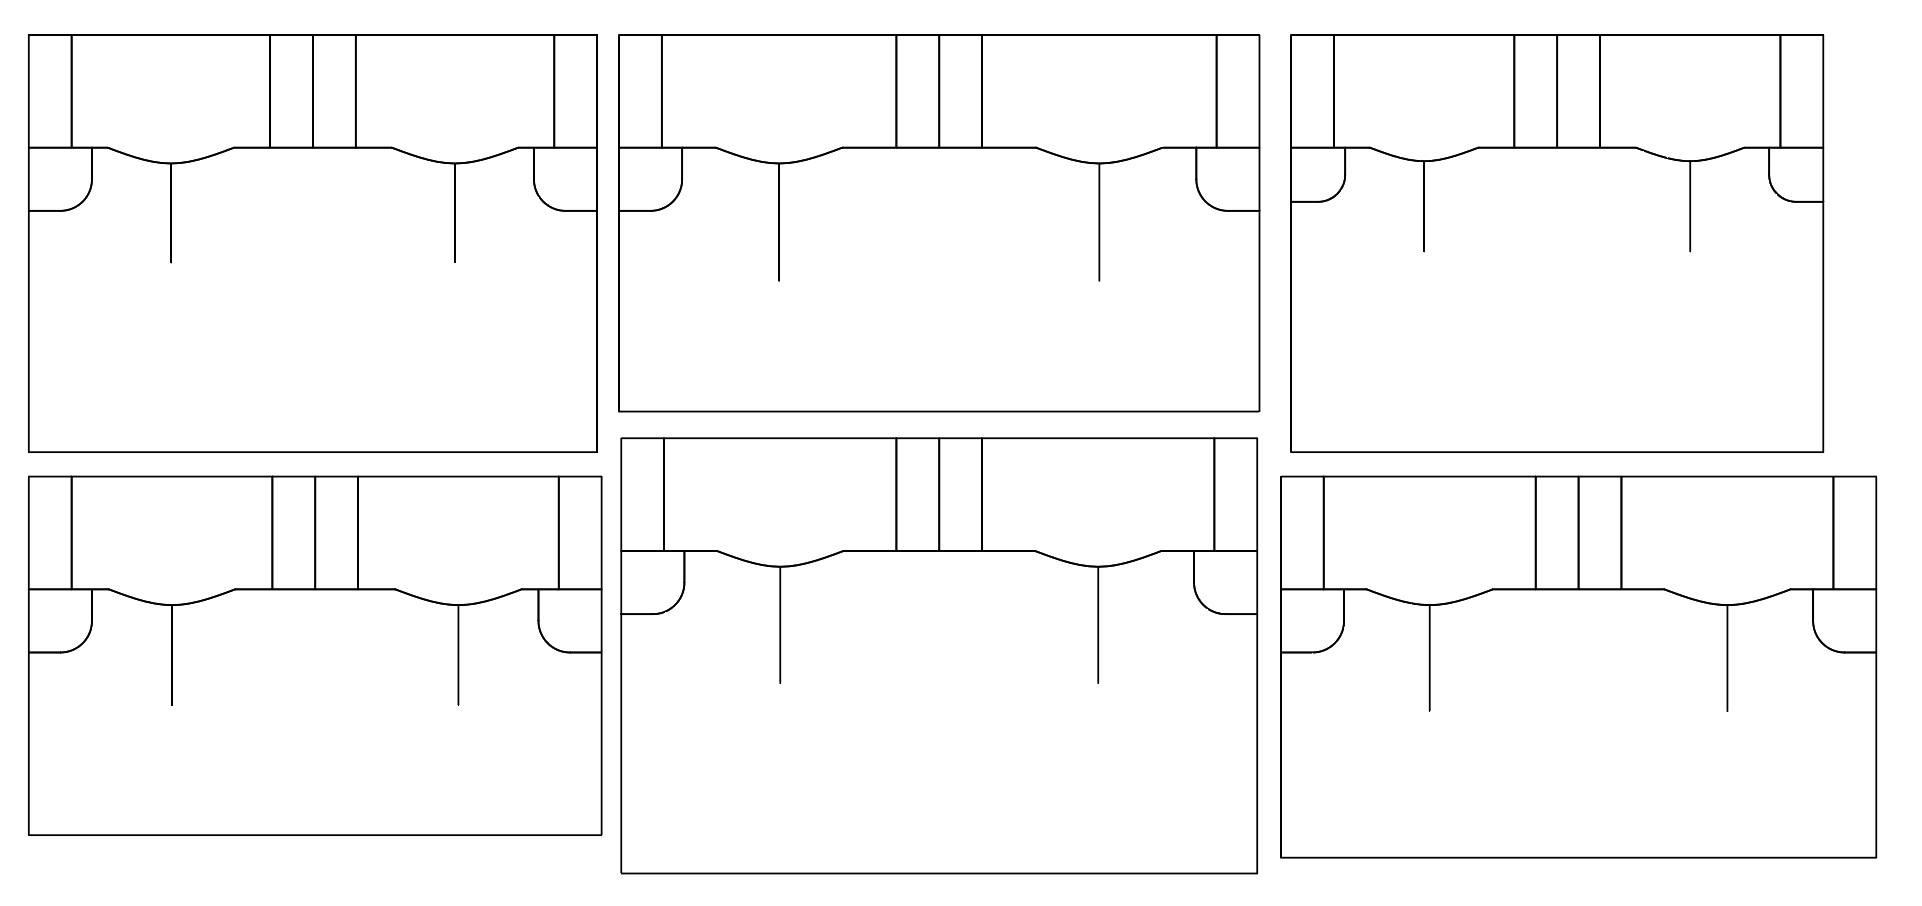
\includegraphics[width = \textwidth]{Images/example dxfs.png}
    \caption{Examples of DXF pattern outputs}
    \label{fig:example dxfs}
\end{figure}

\begin{figure} [H]
    \centering
    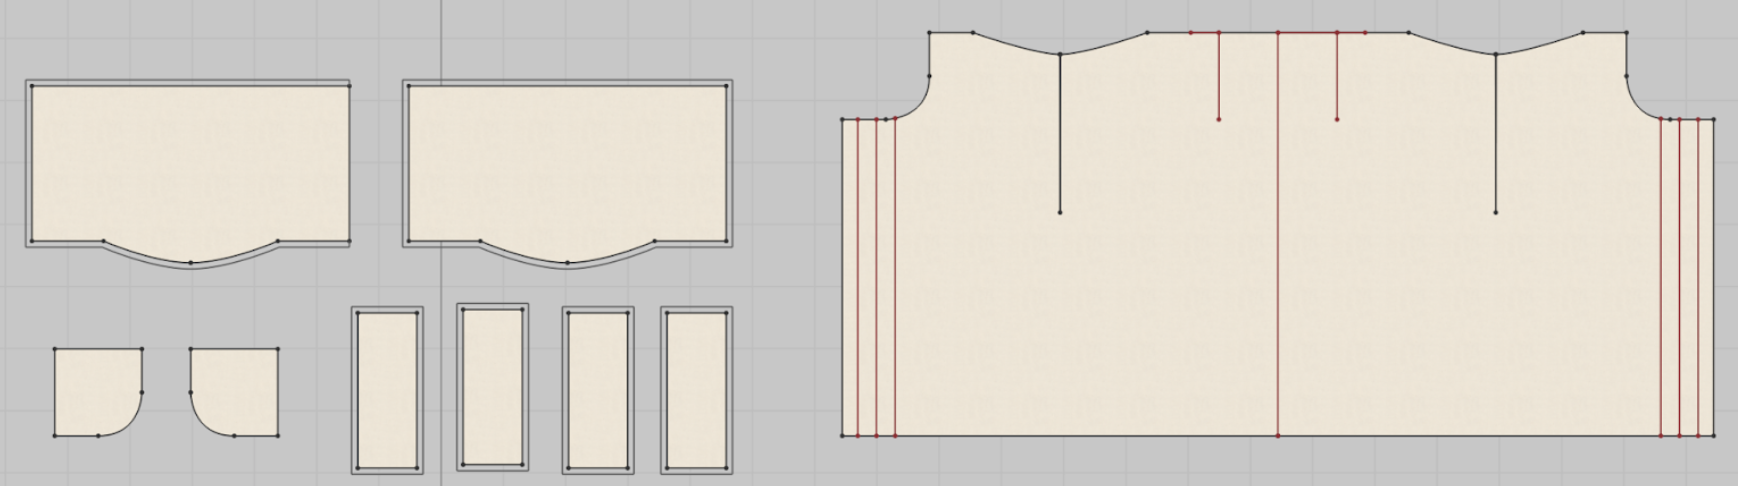
\includegraphics[width = \textwidth]{Images/suc import.png}
    \caption{Successful import in CLO 3D}
    \label{fig:successful import}
\end{figure}

To achieve virtual draping, sew lines need to be defined and pieces positioned around the avatar (Figure \ref{fig:render}). The process requires several steps and for this garment order is as follows: bodice, sleeves, collar, facings.  This achieves the 

\begin{figure} [H]
    \centering
    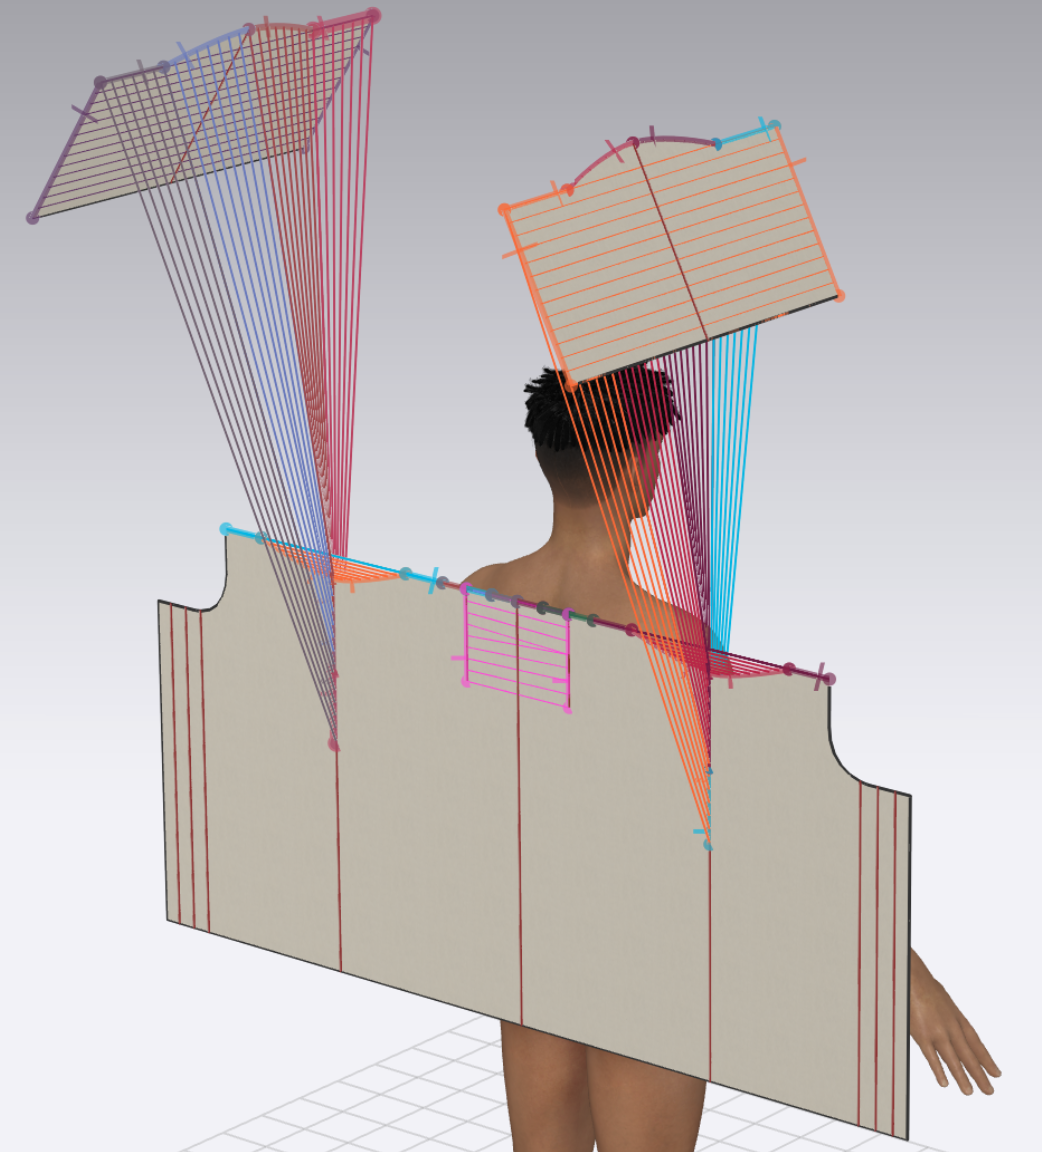
\includegraphics[width = \textwidth]{Images/sew in CLO.png}
    \caption{CLO 3D simulation environment}
    \label{fig:successful import}
\end{figure}

\begin{figure} [H]
    \centering
    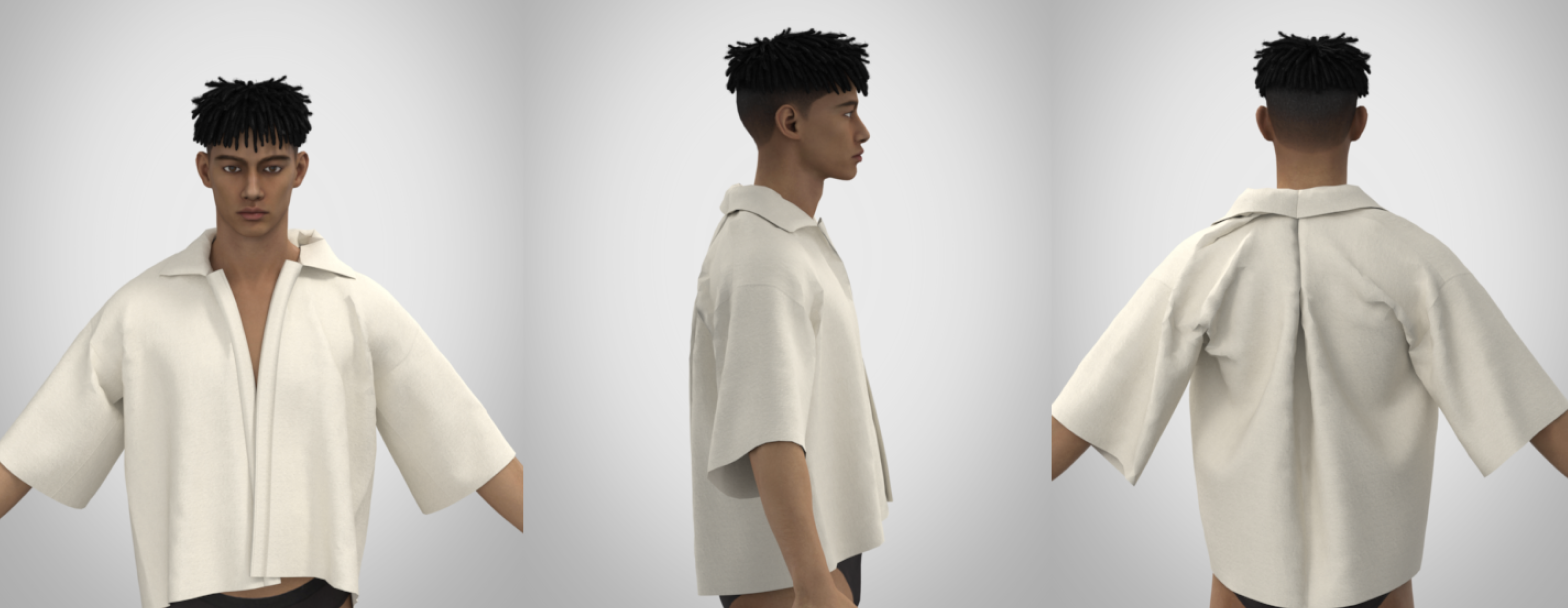
\includegraphics[width = \textwidth]{Images/first render.PNG}
    \caption{Draped garment on preset avatar}
    \label{fig:render}
\end{figure}

\subsubsection{PDF Pattern File}
Along with the DXF file, a PDF file is also provided including annotated dimensions of the pattern. It provides all the information needed for measuring, drawing the pattern pieces, and cutting out pieces from the fabric. It provides the dimensions, parameters, and any unqiue instruction required for the individual The PDF pattern is made by plotting with matplotlib. An example PDF output is shown below.
\begin{figure} [H]
    \centering
    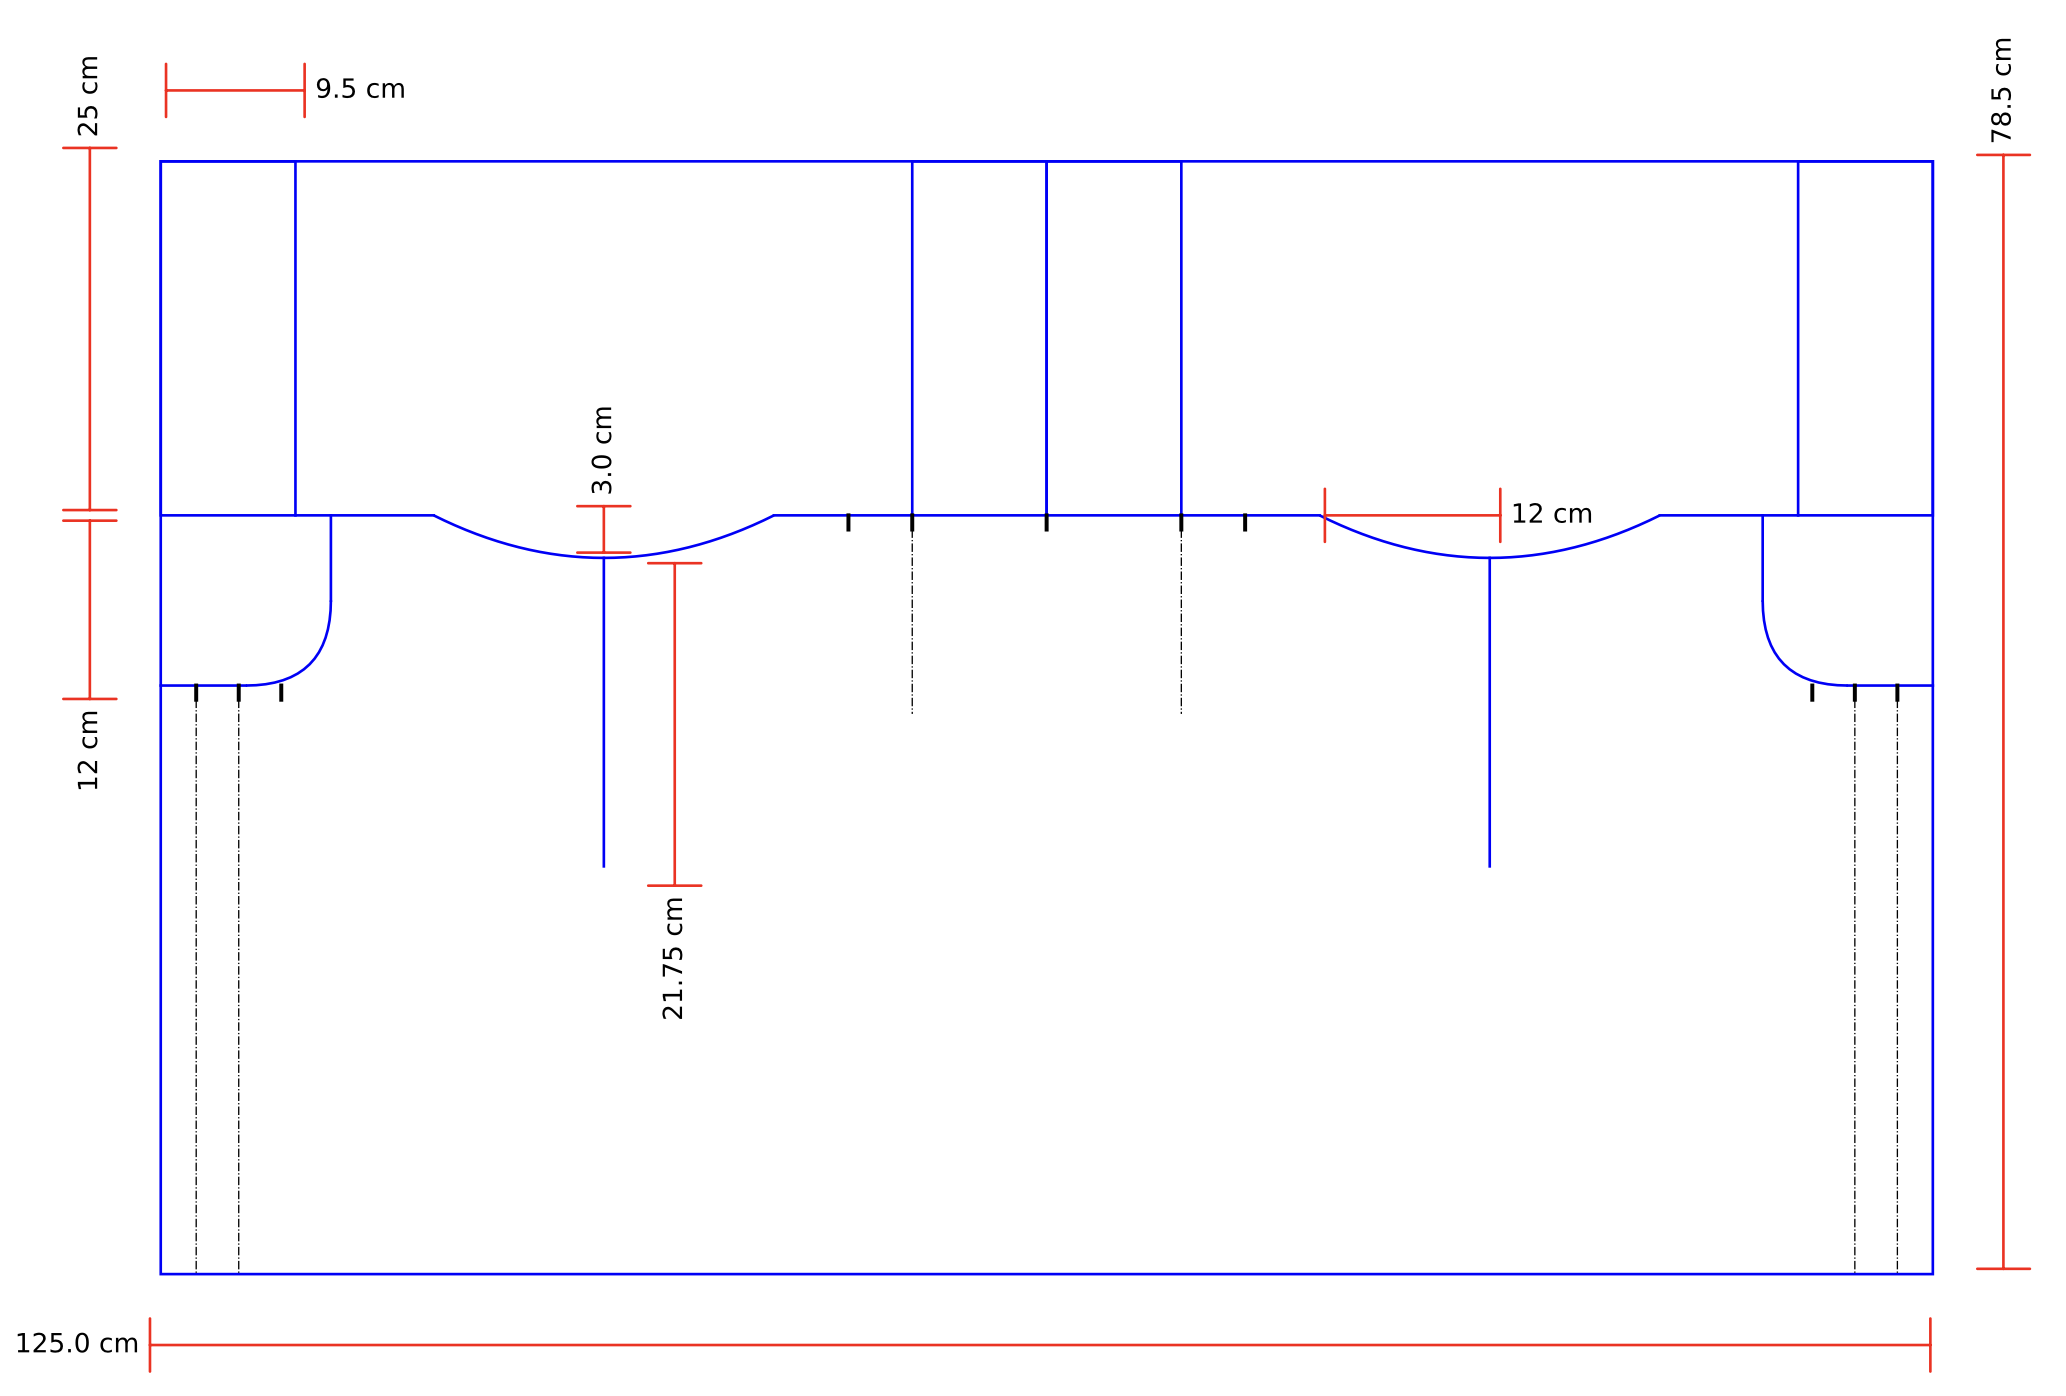
\includegraphics[width = \textwidth]{Images/example pdf output.png}
    \caption{Example PDF pattern output with annotated dimensions}
    \label{fig:pdf output}
\end{figure}

%%%%%%%%%%%%%%%%%%%%%%%%
% FABRIC USE EFFICIENCY
%%%%%%%%%%%%%%%%%%%%%%%%

\subsubsection{Fabric Use Efficiency}
An important goal of this project is to provide the end user independent fashion designer with efficiency metrics given their prior constraints. This makes it possible for them to evaluate different options and make informed decisions.

Initially, the program suggests an industry standard ideal bolt size that minimises waste. There are many different sizes offered and this is dependent on the manufacturer, fabric type, machine used, etc. So we will provide this ideal width assuming you can get in intervals of 5cm. This is also justified as based on Helmersson's size chart. This additional fabric could be used too as increased ease, accepting that compromise to force true zero waste.

The user might want to use a particular bolt of fabric and / or might not want to buy additional fabric of the ideal width. Repurposing and reusing existing materials is always more efficient than going to buy new fabric and the designer should not encourage the purchase of an entire new bolt just so a single garment is made with it. Additionally, the user may have a specific fabric type in mind they want to use that is not available in ideal bolt width. In these cases, the program takes the desired bolt width into account and a separate set of analyses are run (marked with "used" tag).

The 3 options are:
\begin{enumerate}
    \item Pattern width is scaled to fit using ideal bolt width (some minor cut loss)
    \item Pattern width is scaled to zero waste using ideal bolt width (no cut loss)
    \item Pattern width is scaled to fit using available bolt width (cut loss expected)
\end{enumerate}

In all these calculations of waste metrics the assumption is that the user cuts fabric from the bolt roll they are cutting all the way through the fabric width, leaving a clean edge when done cutting from the bolt. The following diagram outlines this.

\begin{figure} [htb]
    \centering
    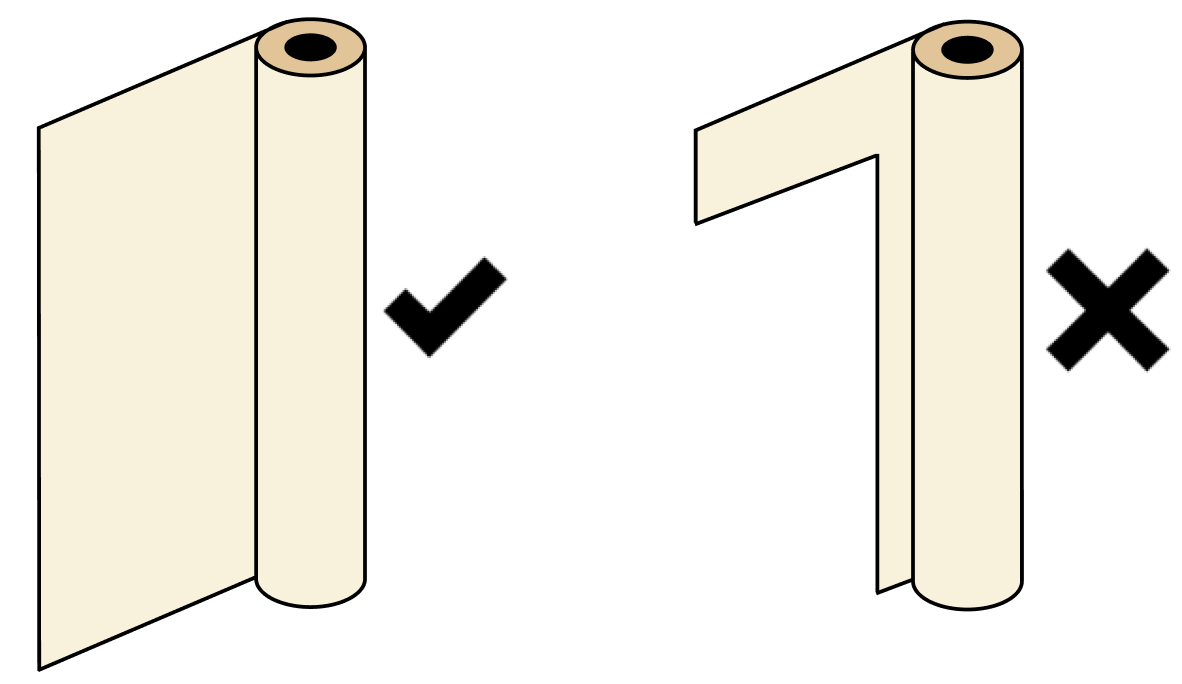
\includegraphics[width = 0.5\textwidth]{Images/bolt cut assumption.png}
    \caption{Cut from bolt assumption}
    \label{fig:cut from bolt}
\end{figure}

The efficiency computation are as follows:

cut loss width = ideal bolt width - pattern width \newline
cut loss area = cut loss width * pattern height \newline
efficiency = 100 * (1 - (cut loss area/ (pattern width * pattern height))

%%%%%%%%%%%%%%%%%%%%%%%%
% MITIGATION
%%%%%%%%%%%%%%%%%%%%%%%%

\subsection{Pattern Segmentation and Reconstruction}
The default assumption is that the pattern width will fall along the bolt width (Figure \ref{fig:pw along bolt})
\begin{figure} [htb]
    \centering 
    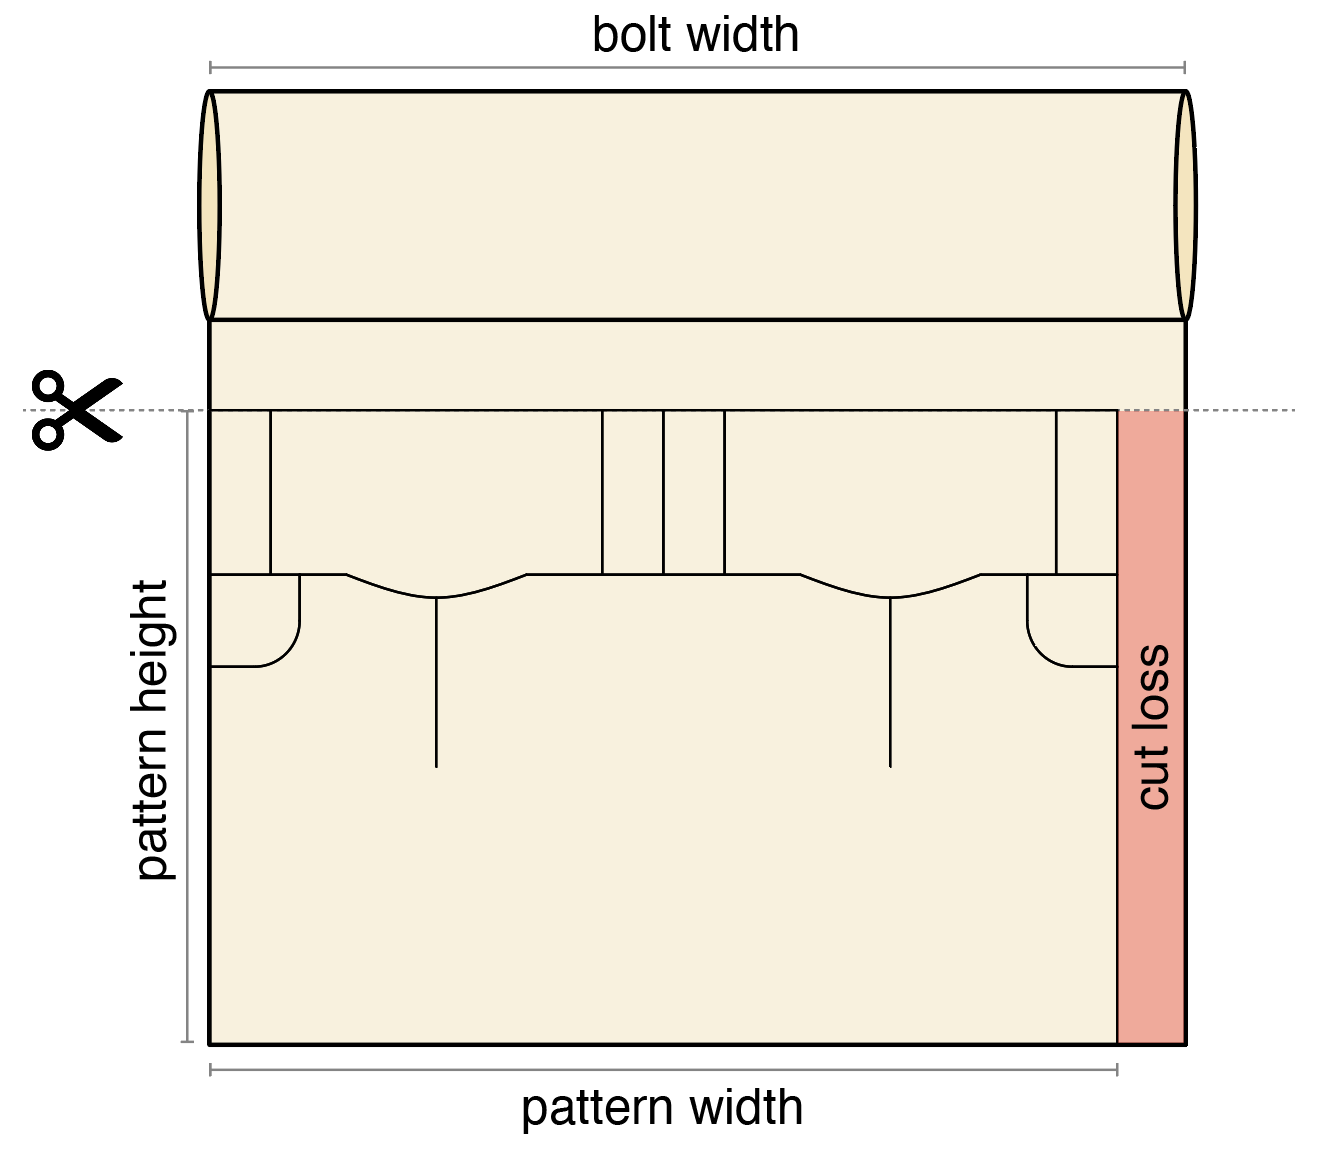
\includegraphics[width = 0.8\textwidth]{Images/regular layout.png}
    \caption{Regular layout}
    \label{fig:pw along bolt}
\end{figure}

If the user prefers a fabric with a bolt width less than pattern width or if the ideal bolt width is unavailable, some mitigation is required. SR technique is employed to realise pattern for larger pattern widths and smaller bolt widths. This will lead to added cut loss and potentially new seams. Complex, sophisticated fitting algoritms are beyong this project's scope. Instead, simple strategies to mitigate the cut loss are provided:

\subsubsection{Rotation}
If the bolt width is greater than pattern height, rotate the pattern 90º (Figure \ref{fig:ph along bolt}).
The waste then becomes:

Waste = (bolt width - pattern height) * pattern width
\begin{figure} [htb]
    \centering
    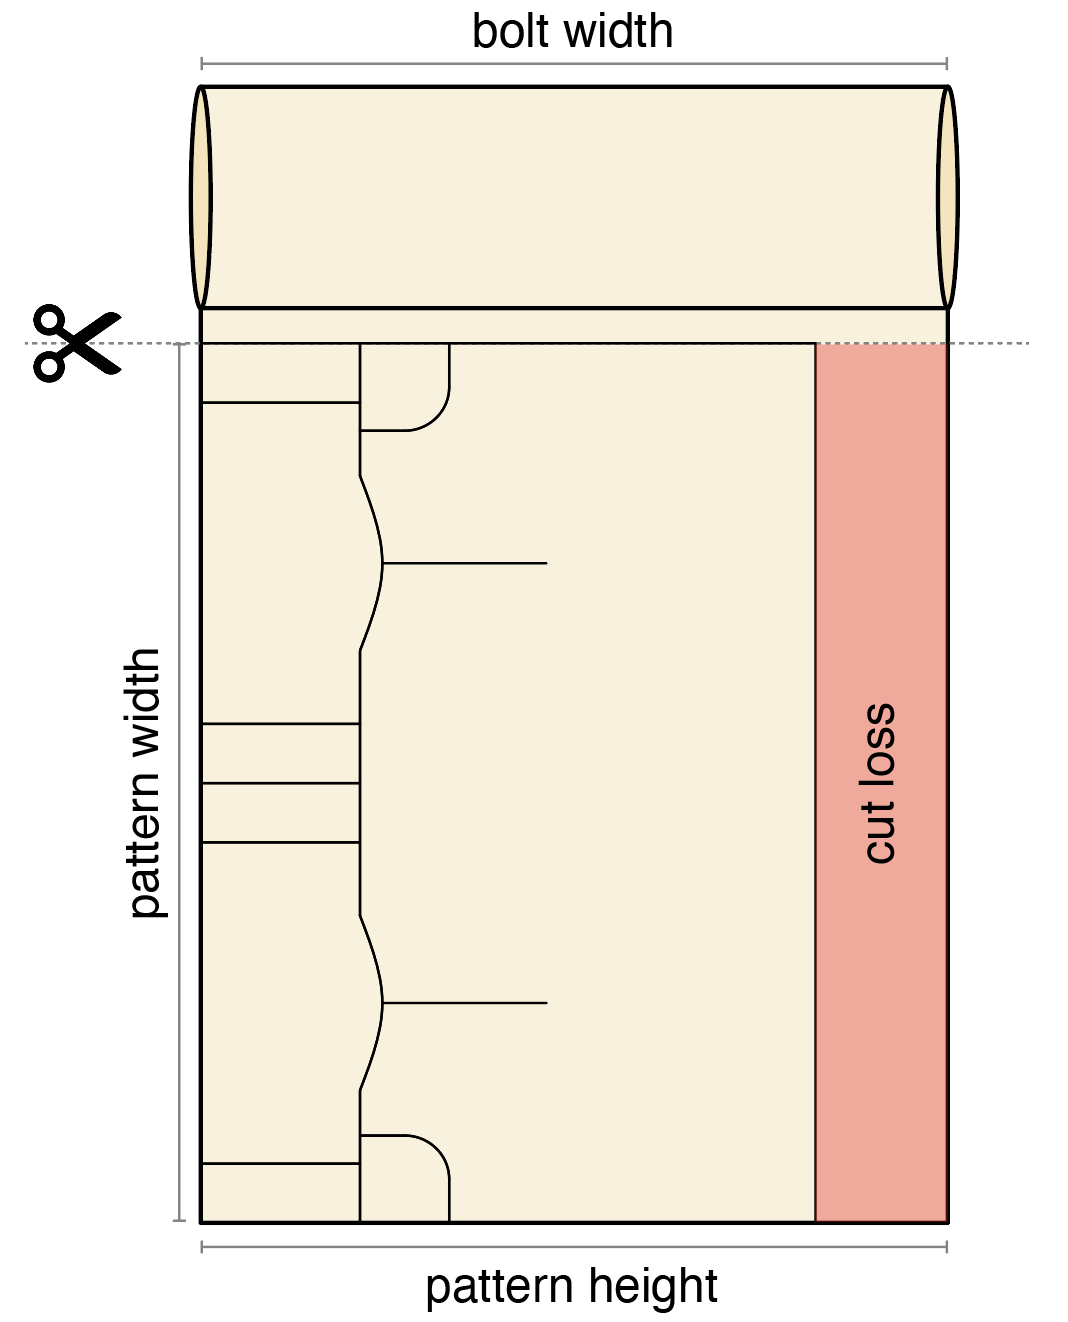
\includegraphics[width = 0.65\textwidth]{Images/rotation layout.png}
    \caption{Rotation layout}
    \label{fig:ph along bolt}
\end{figure}

\subsubsection{Symmetry}
If the bolt width is also less than pattern height, break the pattern into two symmetrical halves along the centre back line (Figure \ref{fig:symmetry split}). This will result in a sewn seam along the centre back in the finished garment and will need a ~1 cm seam allowance. So now each piece has a width equal to half the pattern width plus the seam allowance. The two resultant pieces should be cut from bolt then sewn together along the centre back line first. Then the pattern drawn on and cut.

Resultant piece width = 0.5 * pattern width + seam allowance

The waste then becomes:

Waste = (bolt width - resultant piece width) * 2 * pattern height
\begin{figure} [htb]
    \centering
    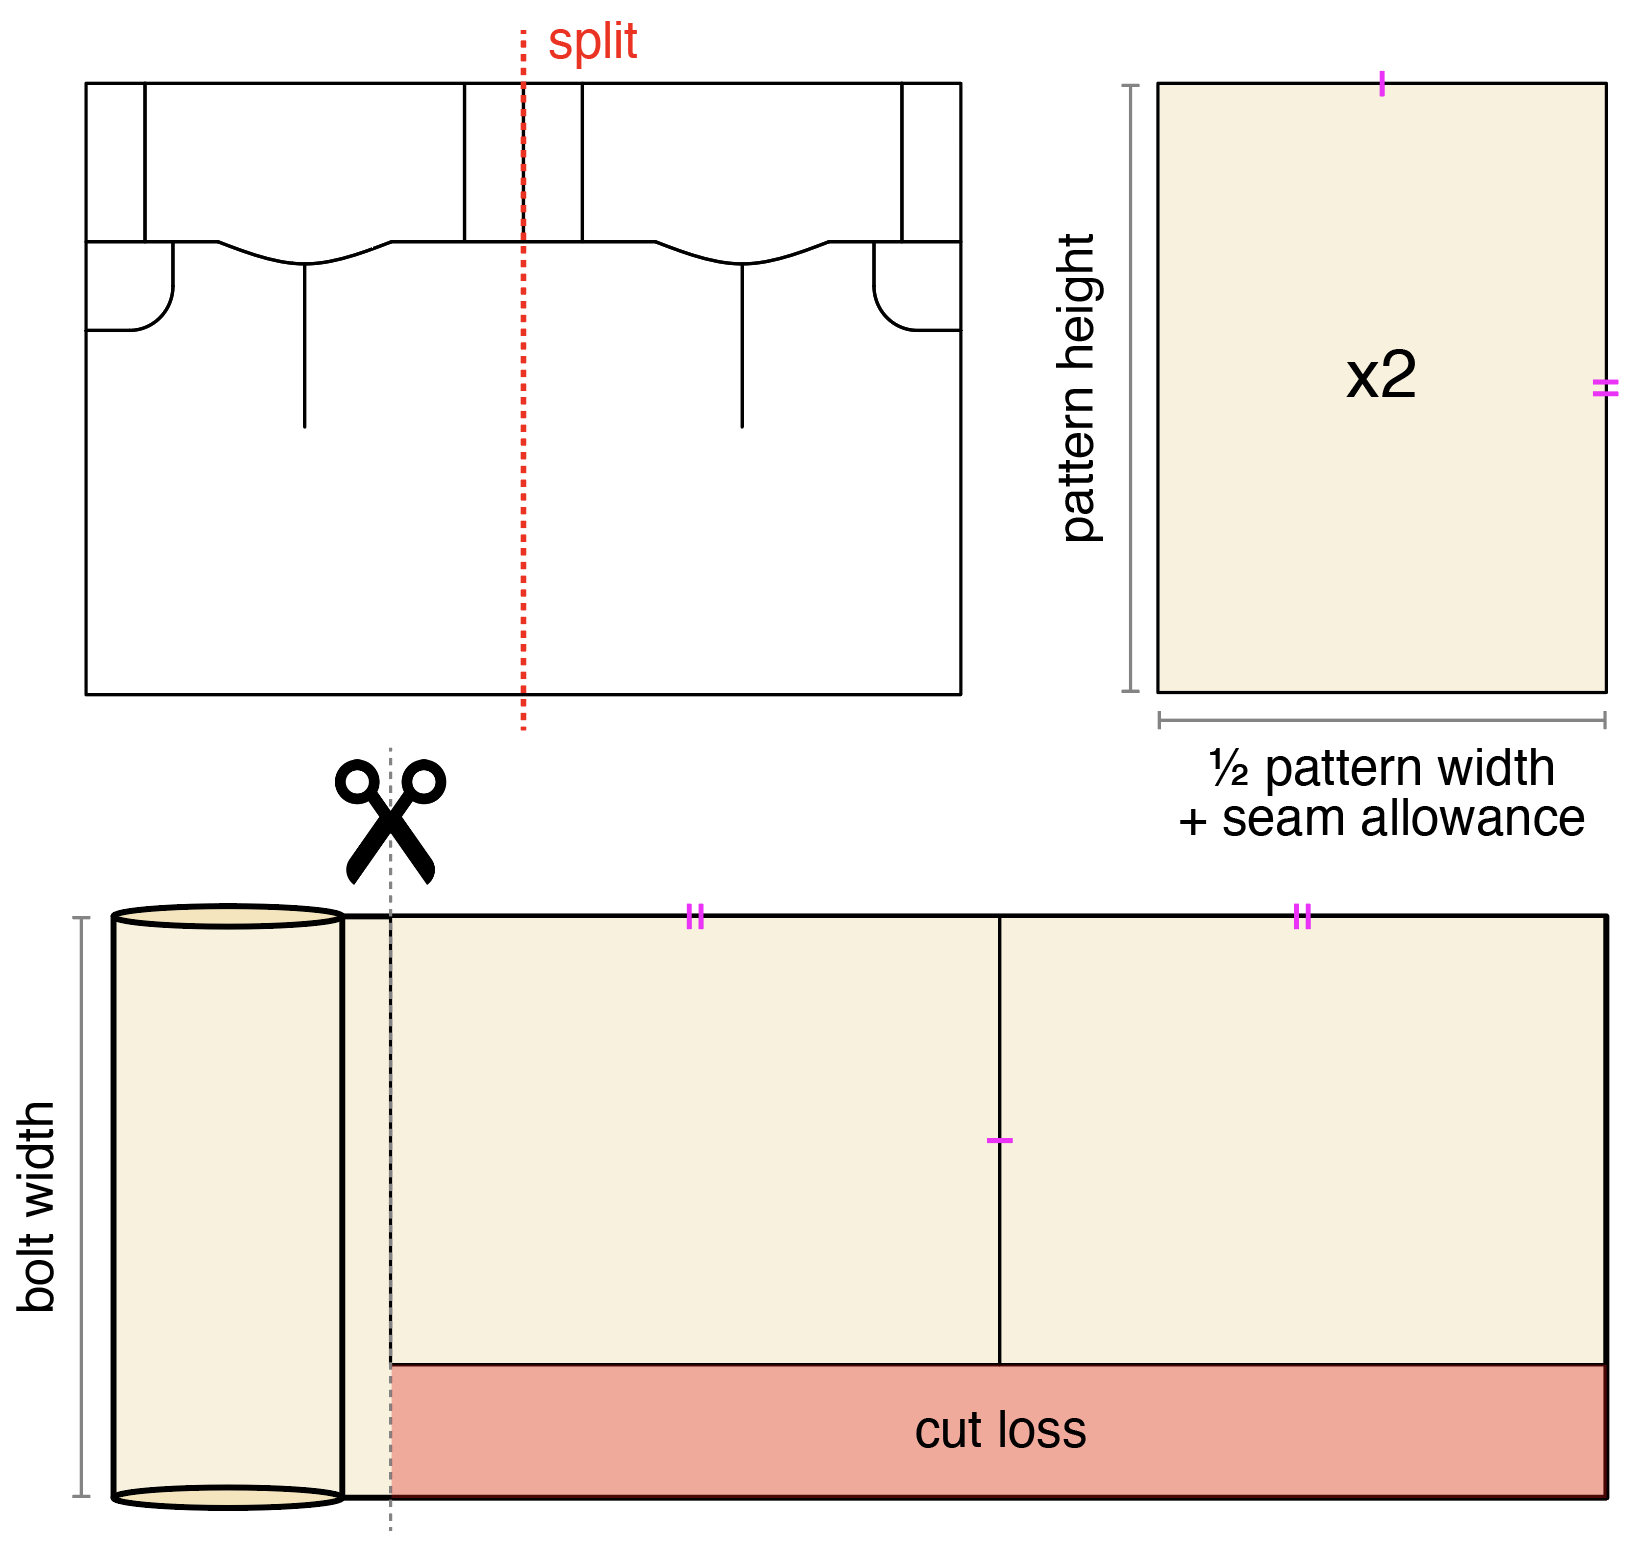
\includegraphics[width = 0.8\textwidth]{Images/symmetry layout.png}
    \caption{Symmetry layout}
    \label{fig:symmetry split}
\end{figure}

\subsubsection{Breakout}
If even the previous resultant piece width is greater than the bolt width then break the pattern into four rectangles. Make a split between the bodice section (inclusive neck facings) and the combined sleeve and collar piece sections along and a split down the centre back line (Figure \ref{fig:breakout}). Pattern height minus the collar piece height (equal to shirt length plus hem allowance) must fit in the bolt for this to work. This has the potential for the most loss but is the tradeoff to use existing fabric from an avaliable smaller width bolt. This will be used in rare occassions where bolt used is significantly smaller than pattern width.
\begin{figure} [htb]
    \centering
    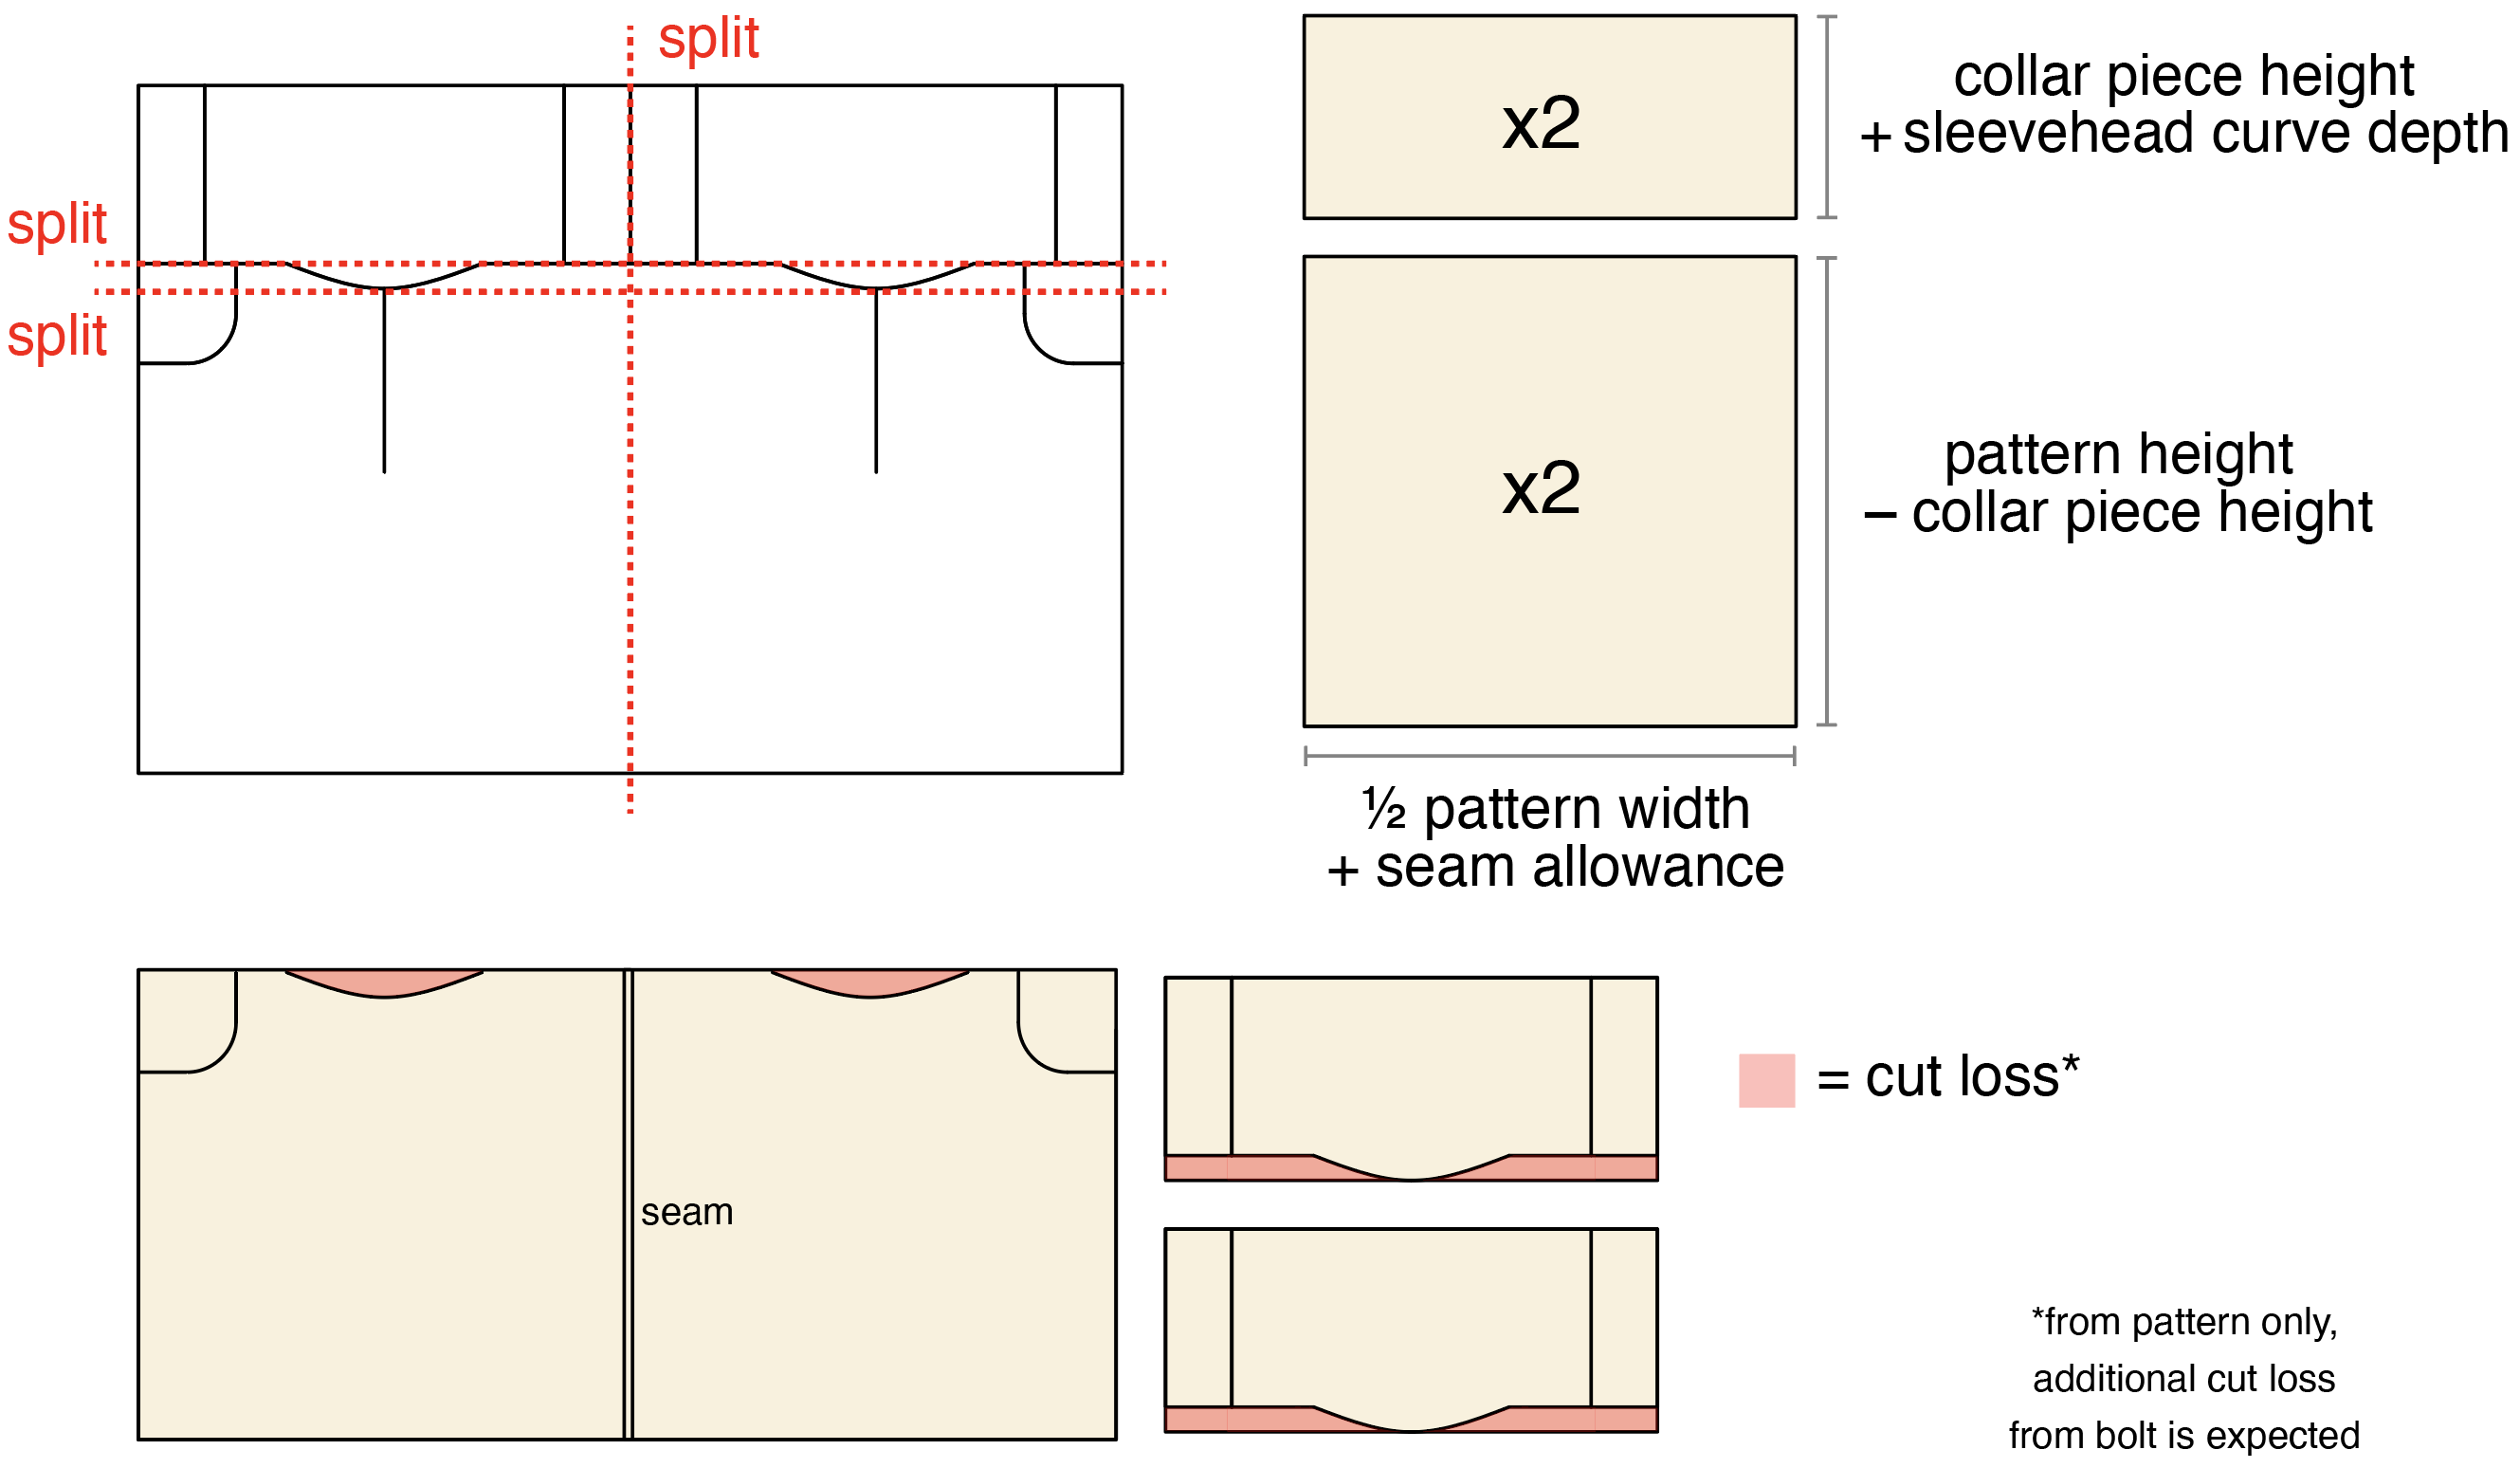
\includegraphics[width = \textwidth]{Images/break out layout.png}
    \caption{Breakout layout}
    \label{fig:breakout}
\end{figure}

%%%%%%%%%%%%%%%%%%%%%%%%
% EMBELLISHMENTS
%%%%%%%%%%%%%%%%%%%%%%%%

\subsubsection{Embellishments}
Even with a rectangular pattern based on the person's dimension, there is always the potential for cut loss. This is especially true if the `ideal bolt width' is not available. One way to recoup this cut loss is via embellishments.

Application of embellishments is highly dependent on the creativity of the fashion designer to generate extra utility by repurposing fabric. Embellishments just cannot be random pieces of fabric tacked onto the garment without a design purpose. For this garment type, front chest pockets are a great embellishment that would well complement the shirt design. 

A standard finished pocket size is 10 cm by 10 cm. Front shirt pockets have sewing and hem allowances that typically are 0.5cm allowance for the sides and bottom edges and 2 cm hem allowance for the top edge to create a quality finish. Adding up these values for a finished pocket, we get a pocket pattern piece that is 11 cm by 12.5 cm. The cut loss width needs to be a minimum of 11 cm to fit the pocket. Smaller sizes, cut up and sewn together to get a finished pocket are not explored due to significantly increased complexity of construction.

This pocket embellishment is an example. The definition of the pocket is customisable. Any fashion designer / sewer can opt for a different size pocket / embellishment. For example a 8 cm by 8 cm finished pocket or a non square 8 cm by 10 cm finished pocket. Its size is not dependent on any body measurement. An example of a body measurement based embellishment is a belt. It would have different dimensions and construction requirements.

For analysis, we just need the dimensions of the embellishment. These are then checked against the cut loss dimension to see if recovery is possible and if so, then compute the percentage amount of the recovery. This analysis can be generalized to any embellishment at all. The only thing that needs to change is the instruction to the sewer on how to tailor this extra piece, of course alongside the new embellishment piece size to check for. An update to the DXF output allows this to be previewed in CLO 3D.

%%%%%%%%%%%%%%%%%%%%%%%%
% WORKSHOP STUDY
%%%%%%%%%%%%%%%%%%%%%%%%
\section{Workshop Study}
\subsection{Purpose}
This study's aim is to test the parameterisation process in a real world setting and evaluate fit and suitability of the parameterisation through qualitative methods. It will evaluate the efficacy of the parameterisation process in creating a better fit for the individual while still keeping its intended style and aesthetic. Focus on fit around the bodice is prioritised. 

The study's dataset will be described using the participants' max bodice circumference measurement and shirt length preference. These are most indicative of the pattern's dimensions and thus resulting waste.

\subsection{Methods}

A digital poster was created for recruitment (see Appendix) and advertised to the DE Fashion and Textiles Research Group, who self-expressed interest in the topic. Participant numbers were limited due to time, resources, and the availability of only three sewing machines. Ethics approval was obtained, and all participants provided informed consent after receiving participant information sheets.

Pattern cutting and sewing instructions, worksheets, and paper patterns were developed for the study/workshop. The workshop was conducted over three 4-hour sessions:

\begin{enumerate}
    \item Initiation: Explained the study schedule and purpose, conducted a paper pattern activity, taught sewing basics, took body measurements, generated bespoke patterns, and cut fabric pieces.
    \item Sewing: Dedicated time for sewing the garment.
    \item Evaluation: Finished the garment and collected qualitative perceptions of fit and comfort.
\end{enumerate}
Body measurements were taken consistently using a provided diagram and instructions (Figure \ref{fig:workshopmeasure}), essential for pattern creation and fit comparison. The workshop focused on making toiles from calico, prototypes made for fit testing. Essential components that allow for wearing like pleats, shoulders, and sleeves were prioritised, while the button placket and collar were pinned for fit evaluation if desired. Once the toile was made, participants wore it for
\begin{figure} [H]
    \centering
    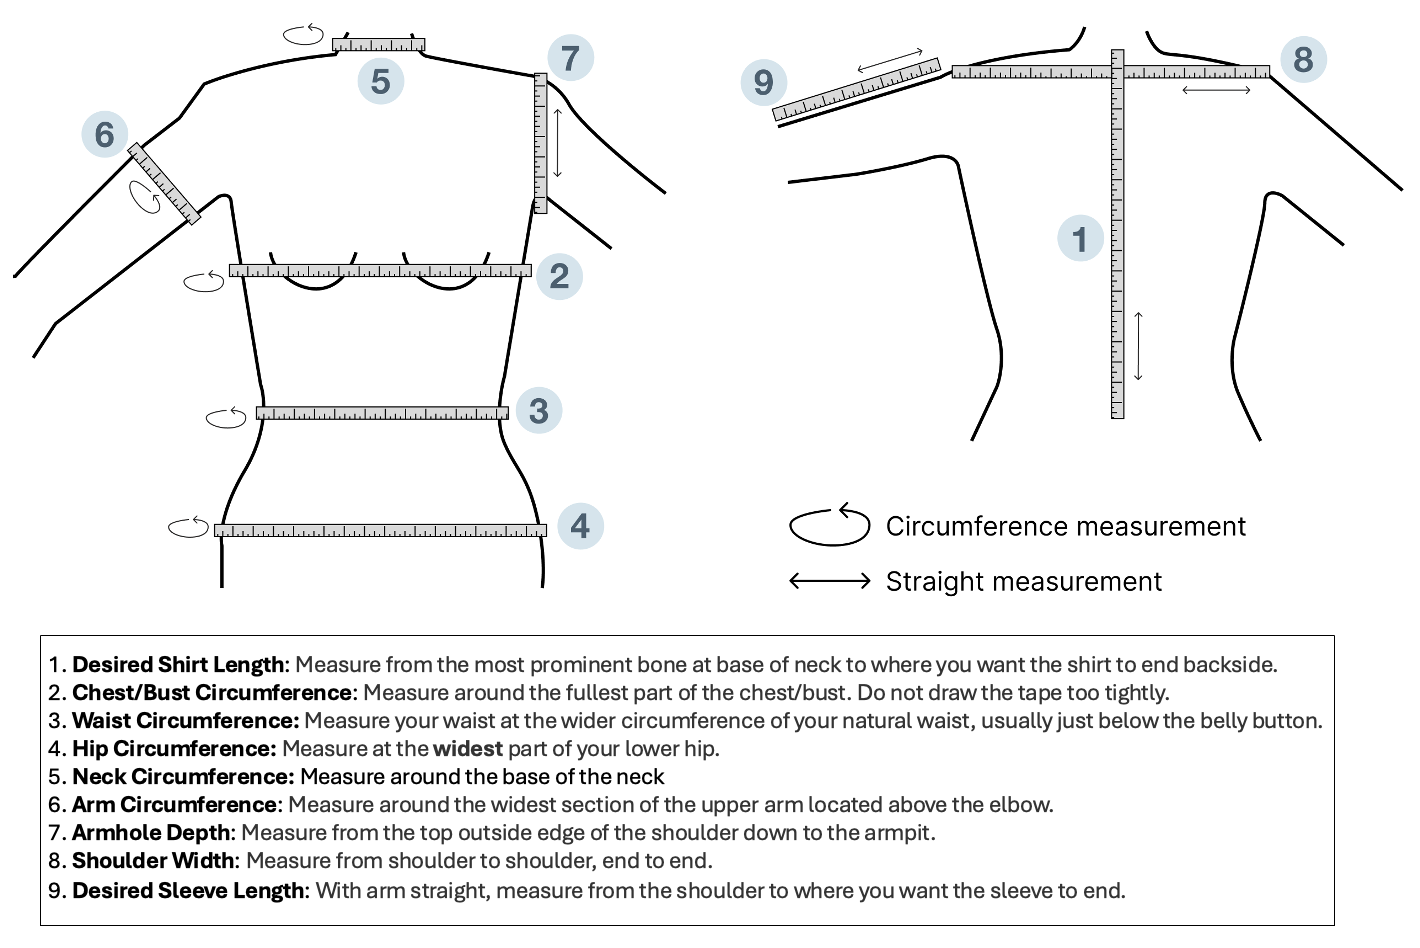
\includegraphics[width = \textwidth]{Images/workshopmeasure.png}
    \caption{Workshop measurement taking instructions}
    \label{fig:workshopmeasure}
\end{figure}


%%%%%%%%%%%%%%%%%%%%%%%%
% BODY SCANS STUDY
%%%%%%%%%%%%%%%%%%%%%%%%
\section{Body Scans Study}
\subsection{Purpose}
This study aims to validate tail0r's processes across a larger dataset than the workshop. Fabric use efficiency metrics and efficacy of pattern segmentation and reconstruction strategies will be computed. No fit analysis will be performed as physical garments will not be produced.

The data comes from the University of Manchester's Apparel Design Engineering (ADE) team. They have made public 100 scans processed using a Size Stream body scanner. The scans are a sample of 20-30 year- old females from the United Kingdom (referred to as the Mendeley dataset).

Similar to the workshop study, the body scan dataset will be described using the max bodice circumference and the shirt length of the participants as these measurements are most indicative of the pattern's dimensions and thus resulting waste.

\subsection{Methods}
The pattern parameterisation methods differ slightly because of the different approach to measurement taking that is carried out by the Size Stream scanner than that of manual measurement taking employed for the workshop. The Size Stream works by

I met with Simeon Gill to discuss and justify the measurements from the scan output that should be used this garment paramterisation. The Mendeley dataset provides many more datapoints and builds measurements from points defined on the body in its 3D space. For the circumference measurements around different areas of the body, the outputted data provides derivatives of the base/driving measurement (usually the circumference). The coding for these derivatives is as follows

c = circumference

TM = tape measure

f = front arc of the circ

b = back arc of the circ

d = depth of the circ

w = width of the circ

h = height of the circ


Tape measure derivatives are useful for our patterns as these bridge concavities of the model as opposed to contours like the "c" coded measurement while closely follows the body surface. To determine the max bodice circumference, we analyse more than just the hip, waist, and chest/bust measurements. In fact, we take into considerations seven relevant bodice circumference TM measurements that reinforce inclusivity of body shapes: Abdomen Circ, Axilla Chest Circ, Chest/Bust Circ, Hip Circ, Seat Circ, Stomach Max Circ, Waist Circ. These are shown in the figures below. The parameterisation still takes the largest of these circumferences and adds the general ease and sew allowance to compute pattern 

The height derivatives are measured from the floor straight up to specified point or arc in the Y plane. The heights of the circumferences are useful because they allow us to derive the relation to where various circumferences are to each other. For the ADE group focusing on more form fitting, non-zero waste clothing, this is useful because this will allow them to control ease around different parts of the body. They can produce a visual representation/estimation of where the body will take up space within the garment. An instance of this is shown in the below example of a bespoke sweatshirt pattern produced by the ADE group. 

For our purposes, the height derivatives will be useful in calculating the pattern height. Since the Mendeley dataset does not provide a center back base neck height and it is not applicable for the person to provide a desired shirt length, a new method for determining shirt length and thus pattern height consistently across all persons was devised.

To calculate the shirt length for the Mendeley scans the following measurements are used: Crotch Height, Waste Height, and Half Back Center TM. The Half Back Center TM extends from the the back neck landmark to the center back waist landmark measured along the contour of the back, seen in the image below. The back waist landmark is a point on the waist circumference so using the derivative waist height from it is appropriate. An important note is that the waist height and crotch height are straight lines and the half back center TM is a contour. Consultation with Simeon Gill decided that this will not affect the outcome greatly (being slightly longer shirt length than if the half back center measurment was a straight line) and is suitable for purposes of finding a consistent method of shirt length given we cannot get a desired input).
% \begin{figure} [H] % opens the figure environment. the '[H]' forces the image to be Here
%     \centering % puts the image in the horizontal centre of the page
%     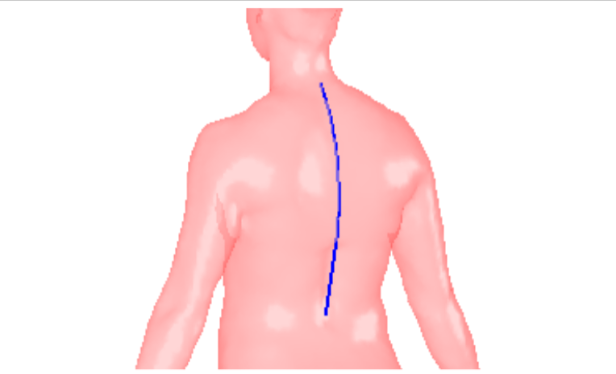
\includegraphics[width = 0.5\textwidth]{Images/HBC TM.png} %this tells latex what graphics to include. I put my images in an 'Images' folder to aid file management, hence the Images/ before the file name. the width bit before allows you to alter the width of the image. It is also possible to use scale as well as using equations with the textwidth to make it say half the text width.
%     \caption{Half Back Center TM diagram}
% \end{figure}
To calculate the shirt length, we will add the waist height to the half back center and substract the crotch height from it.

Shirt Length = Waist Height + Half Back Center TM - Crotch Height

This will be treated as the desired shirt length and plugged in to the pattern height formula as stated before in section 3.2. 

This data is run through the program to calculate the fabric use efficiencies and verify suitability of the pattern file construction.

\section{Personal Case Study}
\subsection{Purpose}
The purpose of this study is to take an individual scan and parameterise the garment to verify its draping virtually as well as physically with a sewn garment. This is a mixed mode study where tailoring measurements are taken from scan data and actual and virtual garments are evaluated for fit.

There is some utility in draping on a generic 3D avatar, however evaluating fit is better on a personalised scan, akin to seeing clothes on a mannequin versus trying them on. This is an example of research through design to complement the methodology of the other studies.

\subsection{Methods}
The author got their own scan data from the ADE group in Manchester. Pattern parameterisation differs slightly due to slightly different data points provided. The data did not provide an Axilla Chest circumference and was omitted from max bodice circumference computation. 

Also data did not have a half back centre measurement but did provide the neck base circumference. The height derivative of the neck base circumference was used and the crotch height subtracted from it to get the desired shirt length. This is consistent with the method used in 3.4. 
Shirt Length = Neck Base Height - Crotch Height
					
The median values of the measurements from 5 total scans were used in the pattern's parameterisation to account for variability that could arise from factors such as posture, breathing, and slight movements during scanning.

\chapter{Results}

\section{Workshop Study}
The workshop study had eight participants a mean maximum bodice circumferemce of 99.96 cm, median of 98.50 cm and a standard deviation of 8.00 cm. The mean shirt length is 60.36 cm, median of 59.70 cm, and a standard deviation of 6.99 cm. Six of eight completed the entire study, reaching finished garment stage and fit evaluation. Their garments are seen in Figure \ref{fig:workshop_garments}
\begin{figure}[htb]
    \centering
    \begin{subfigure}[b]{0.45\textwidth}
        \centering
        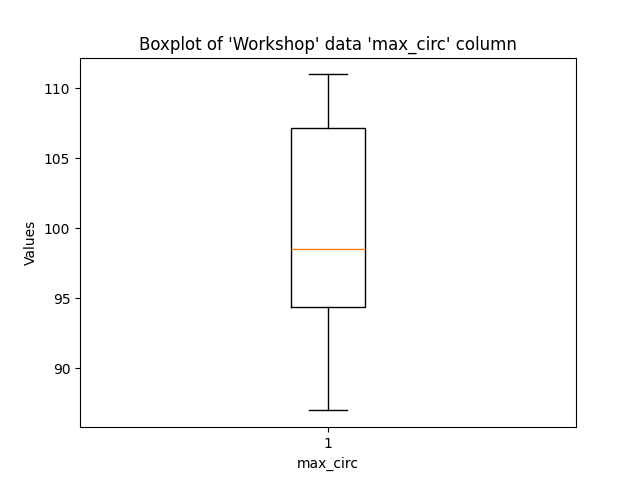
\includegraphics[width=\textwidth]{Images/Workshop_max_circ_Boxplot.png}
        \caption{}
    \end{subfigure}
    \hfill
    \begin{subfigure}[b]{0.45\textwidth}
        \centering
        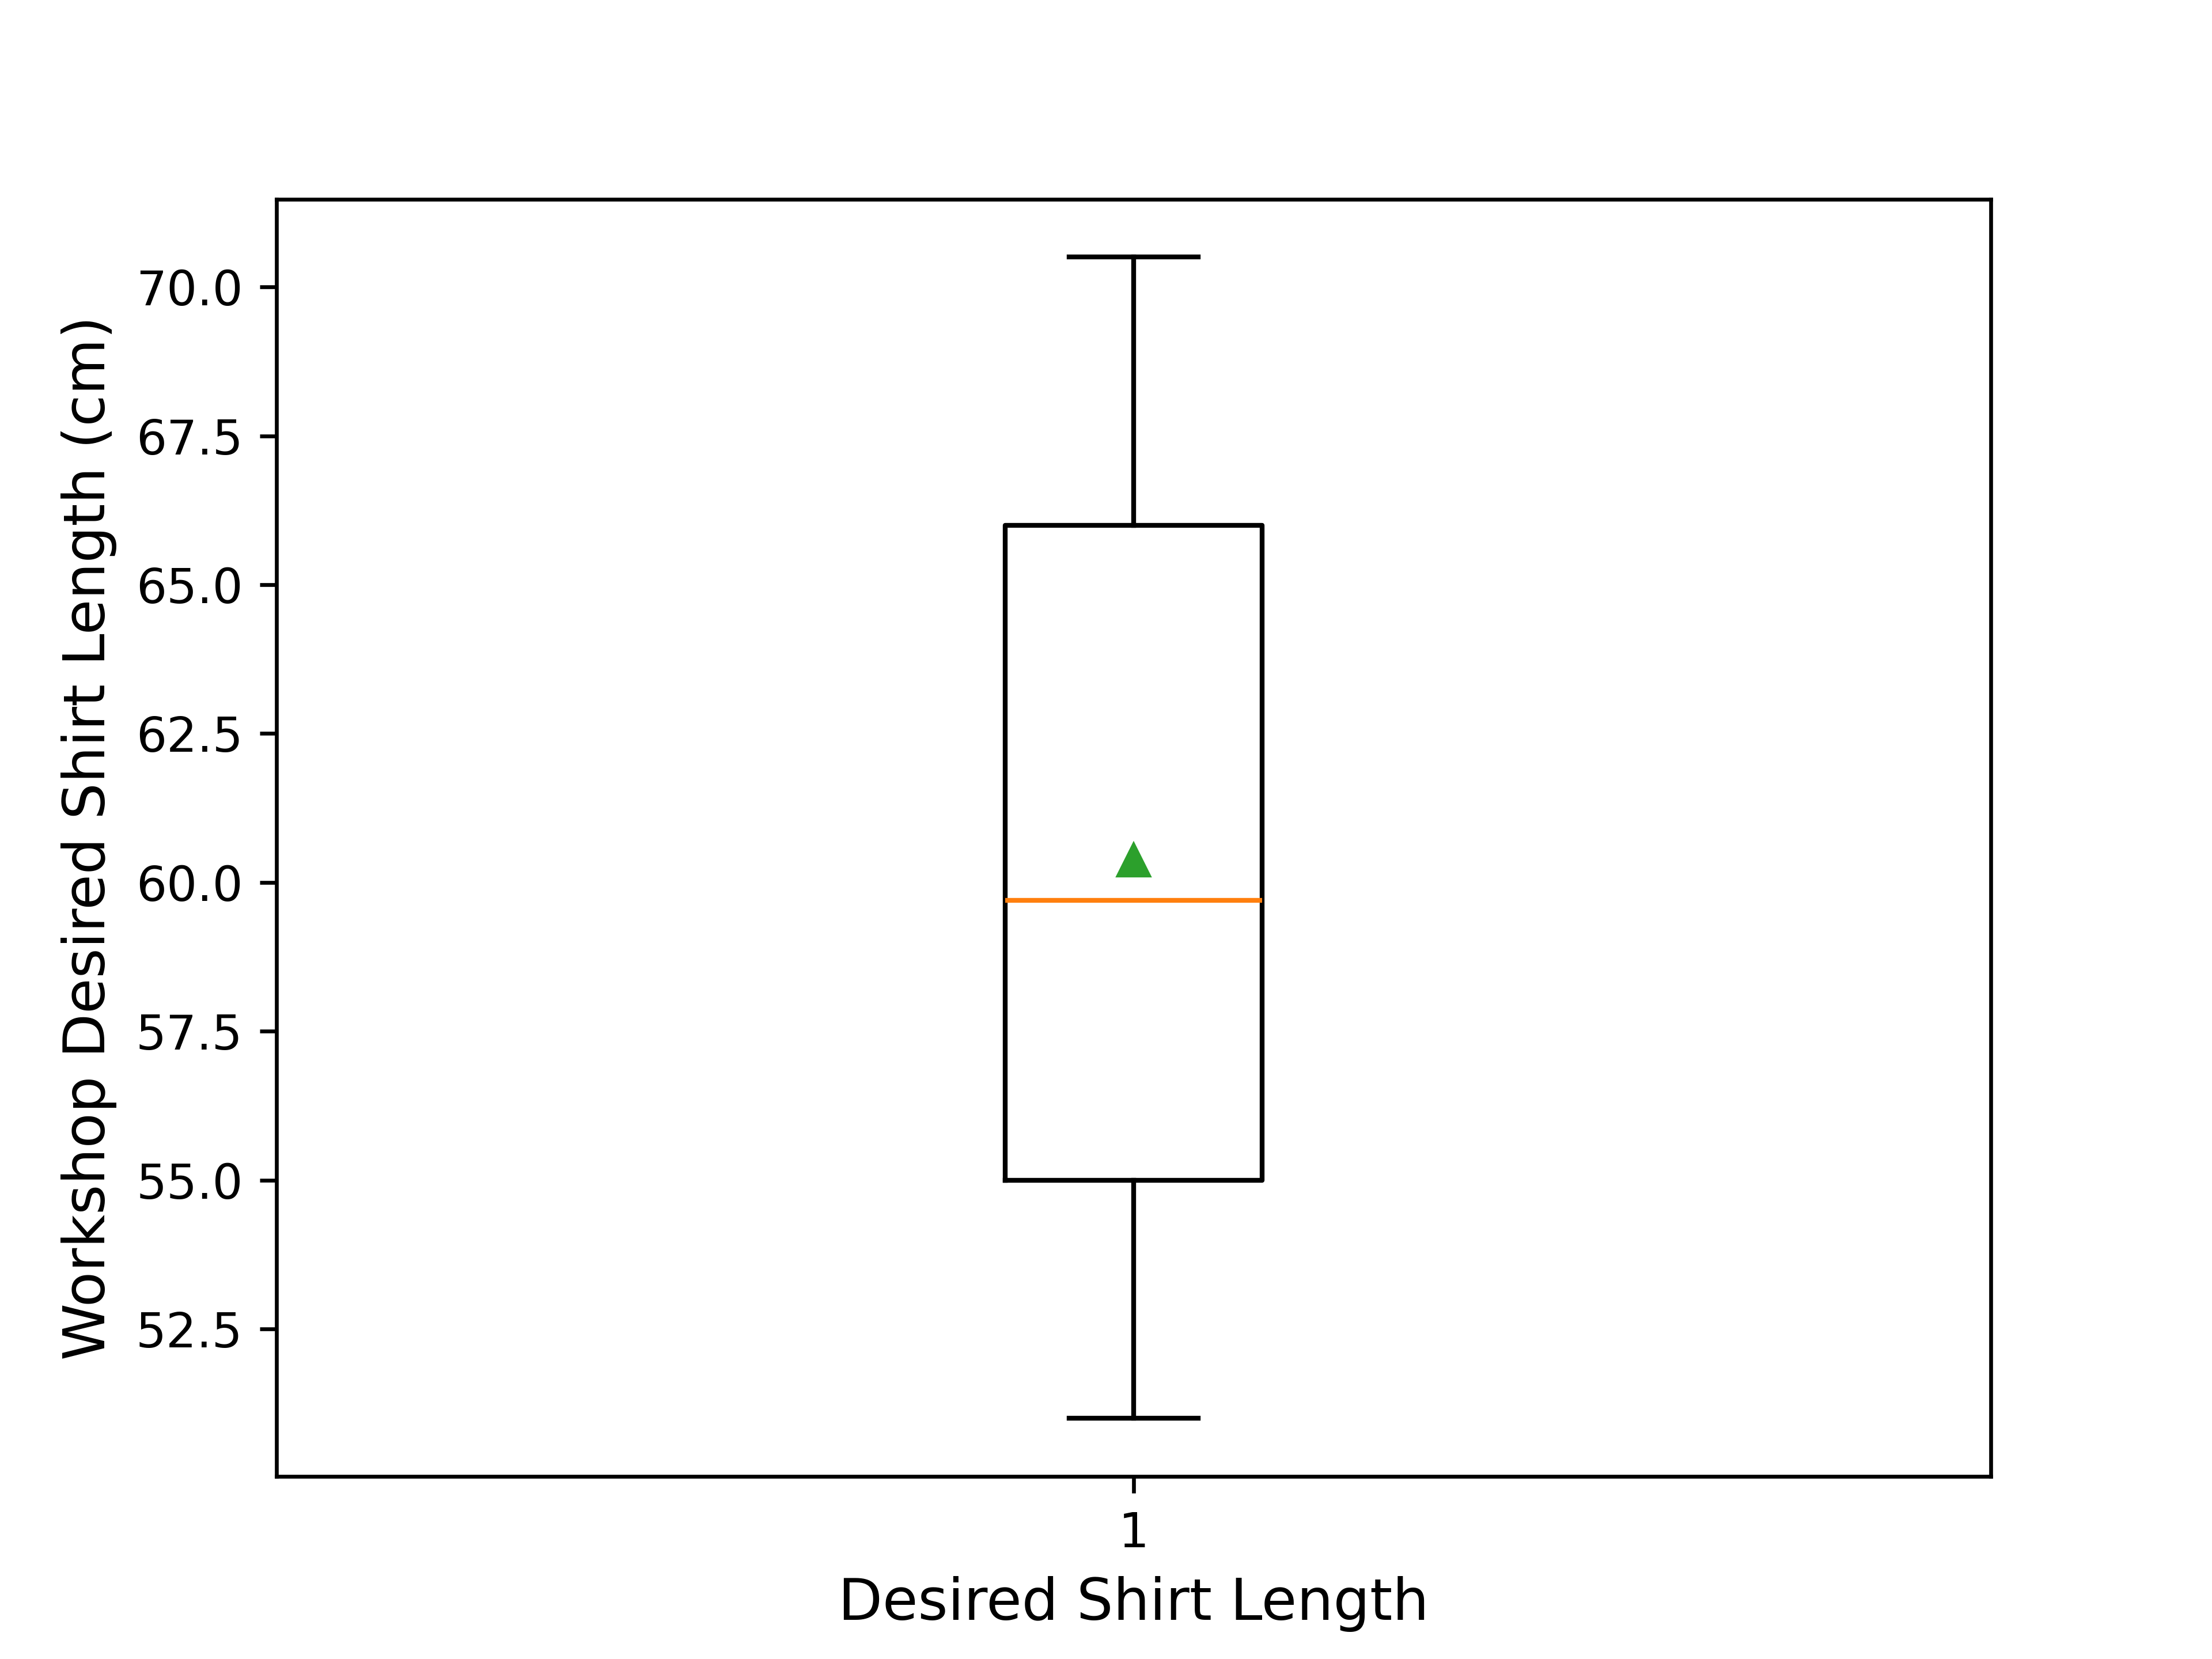
\includegraphics[width=\textwidth]{Images/Workshop_desired_shirt_length_Boxplot.png}
        \caption{}
    \end{subfigure}
    \caption{}
\end{figure}
\newpage
\begin{figure} [H]
    \centering
    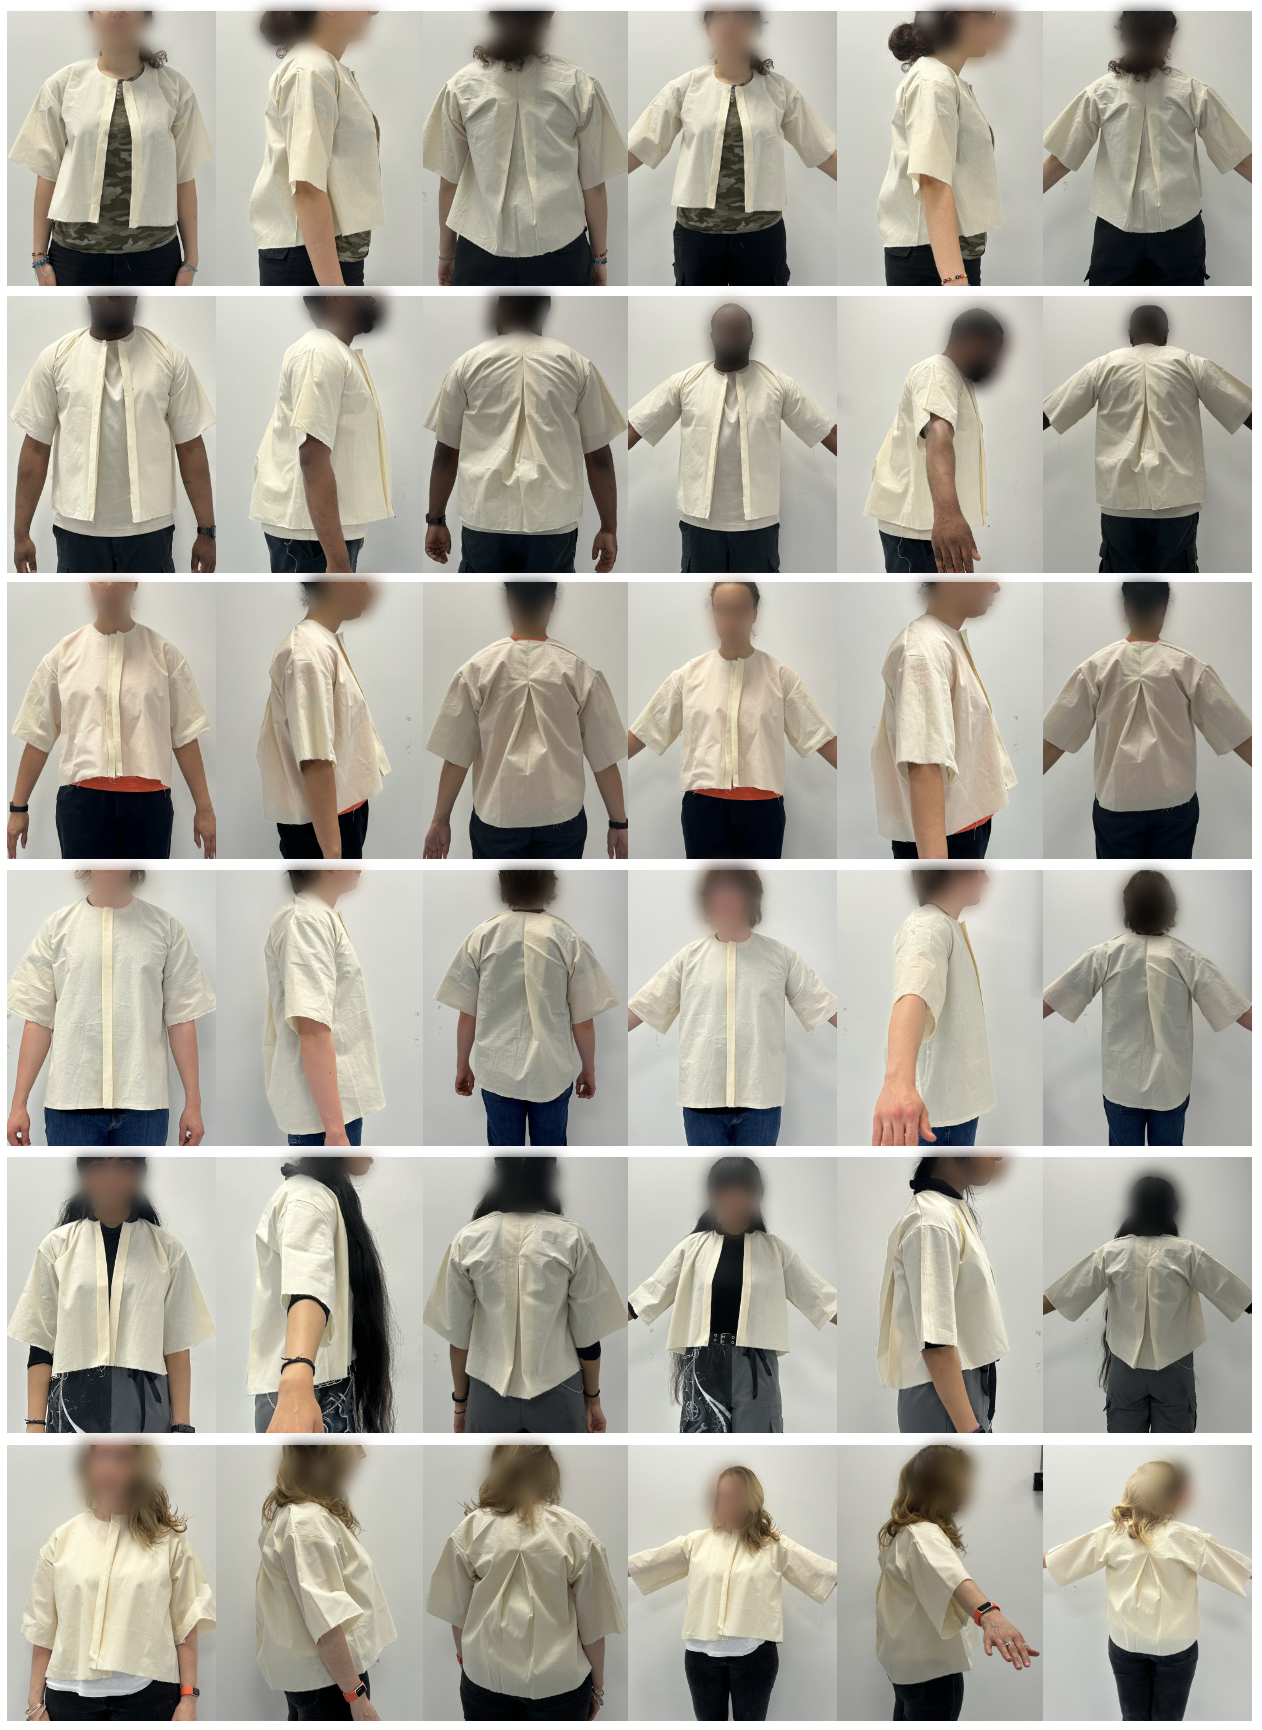
\includegraphics[width = \textwidth]{Images/workshop garments.png}
    \caption{Workshop study garments}
    \label{fig:workshop_garments}
\end{figure}

\begin{figure} [H]
    \centering
    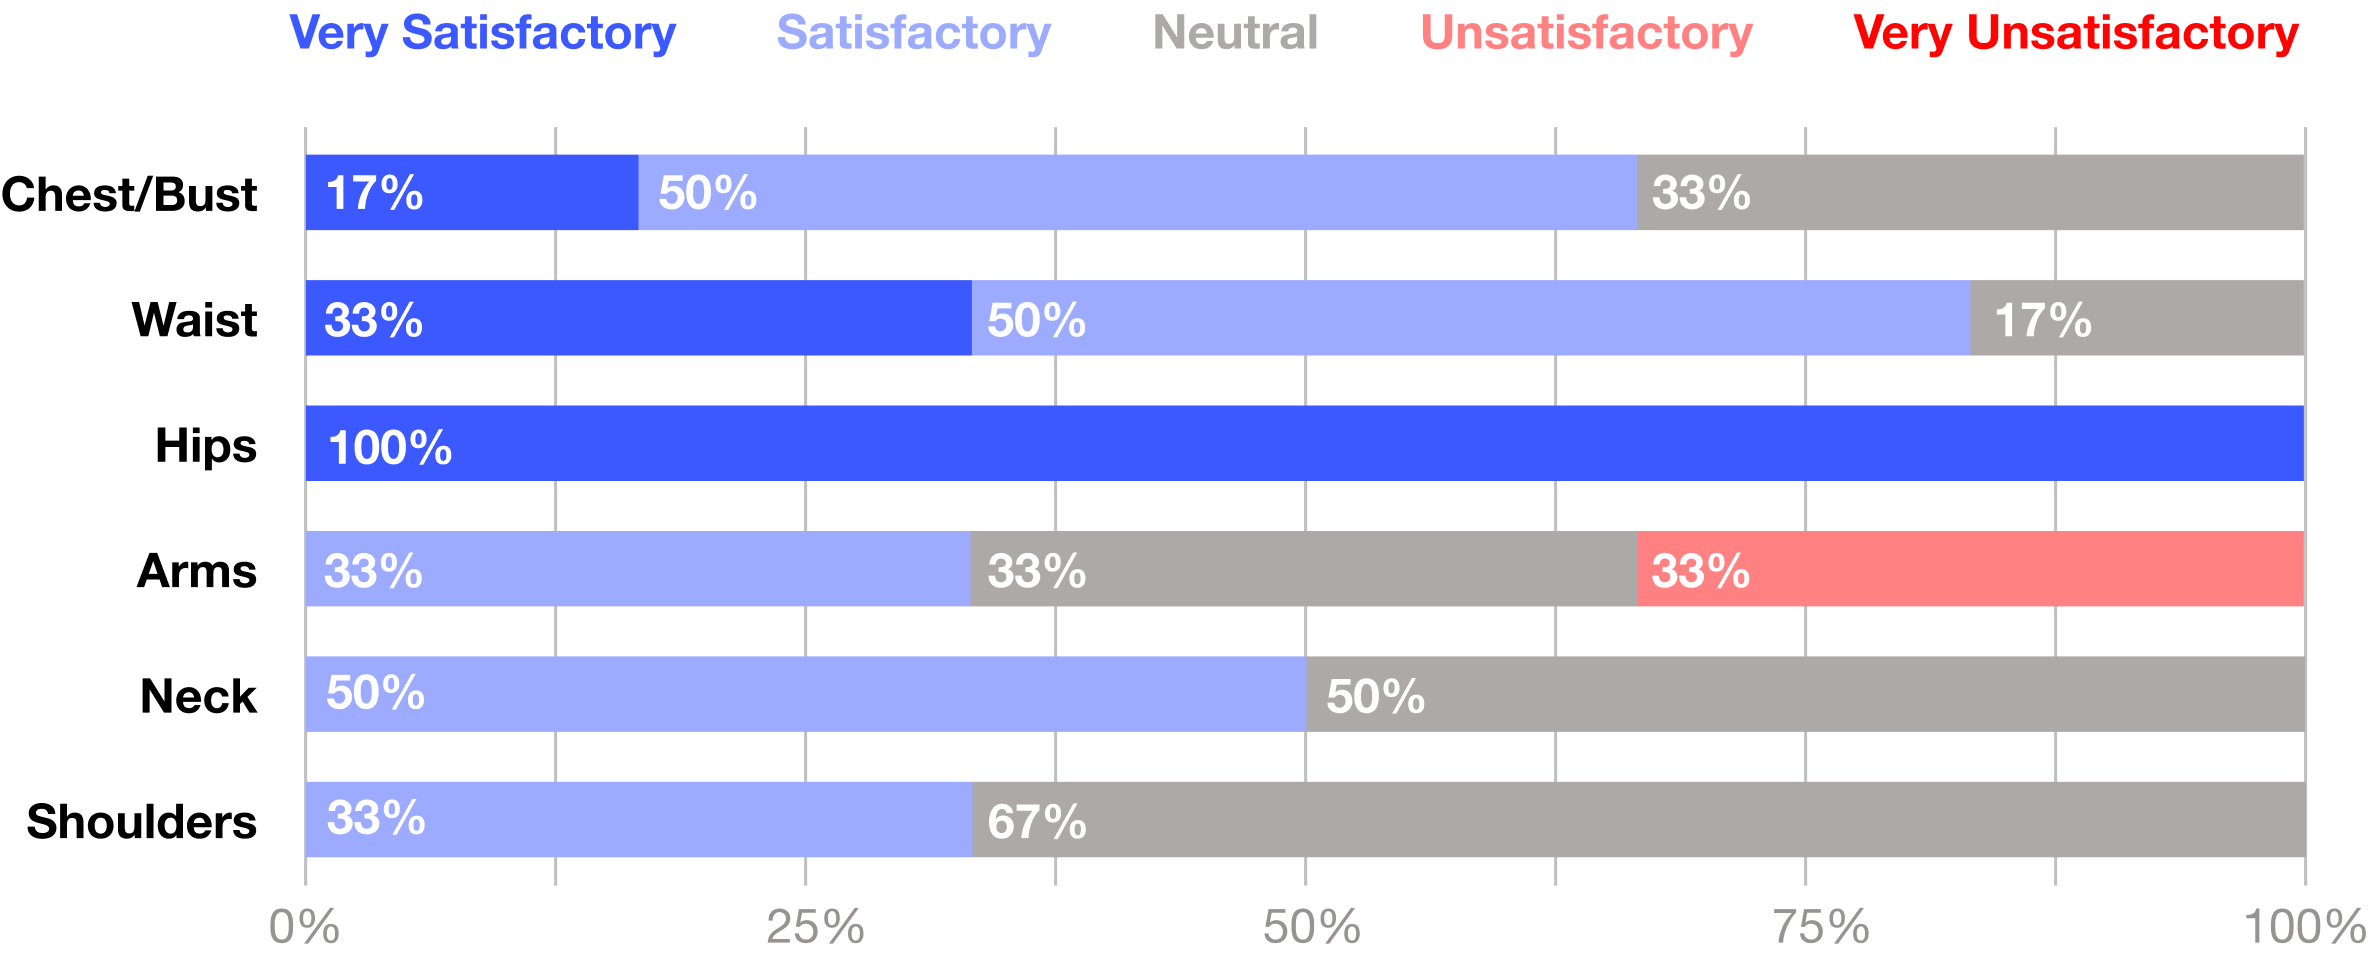
\includegraphics[width = 0.8\textwidth]{Images/fit likert stacked bar.png}
    \caption{Fit Likert Scales}
\end{figure}
\begin{figure} [H]
    \centering
    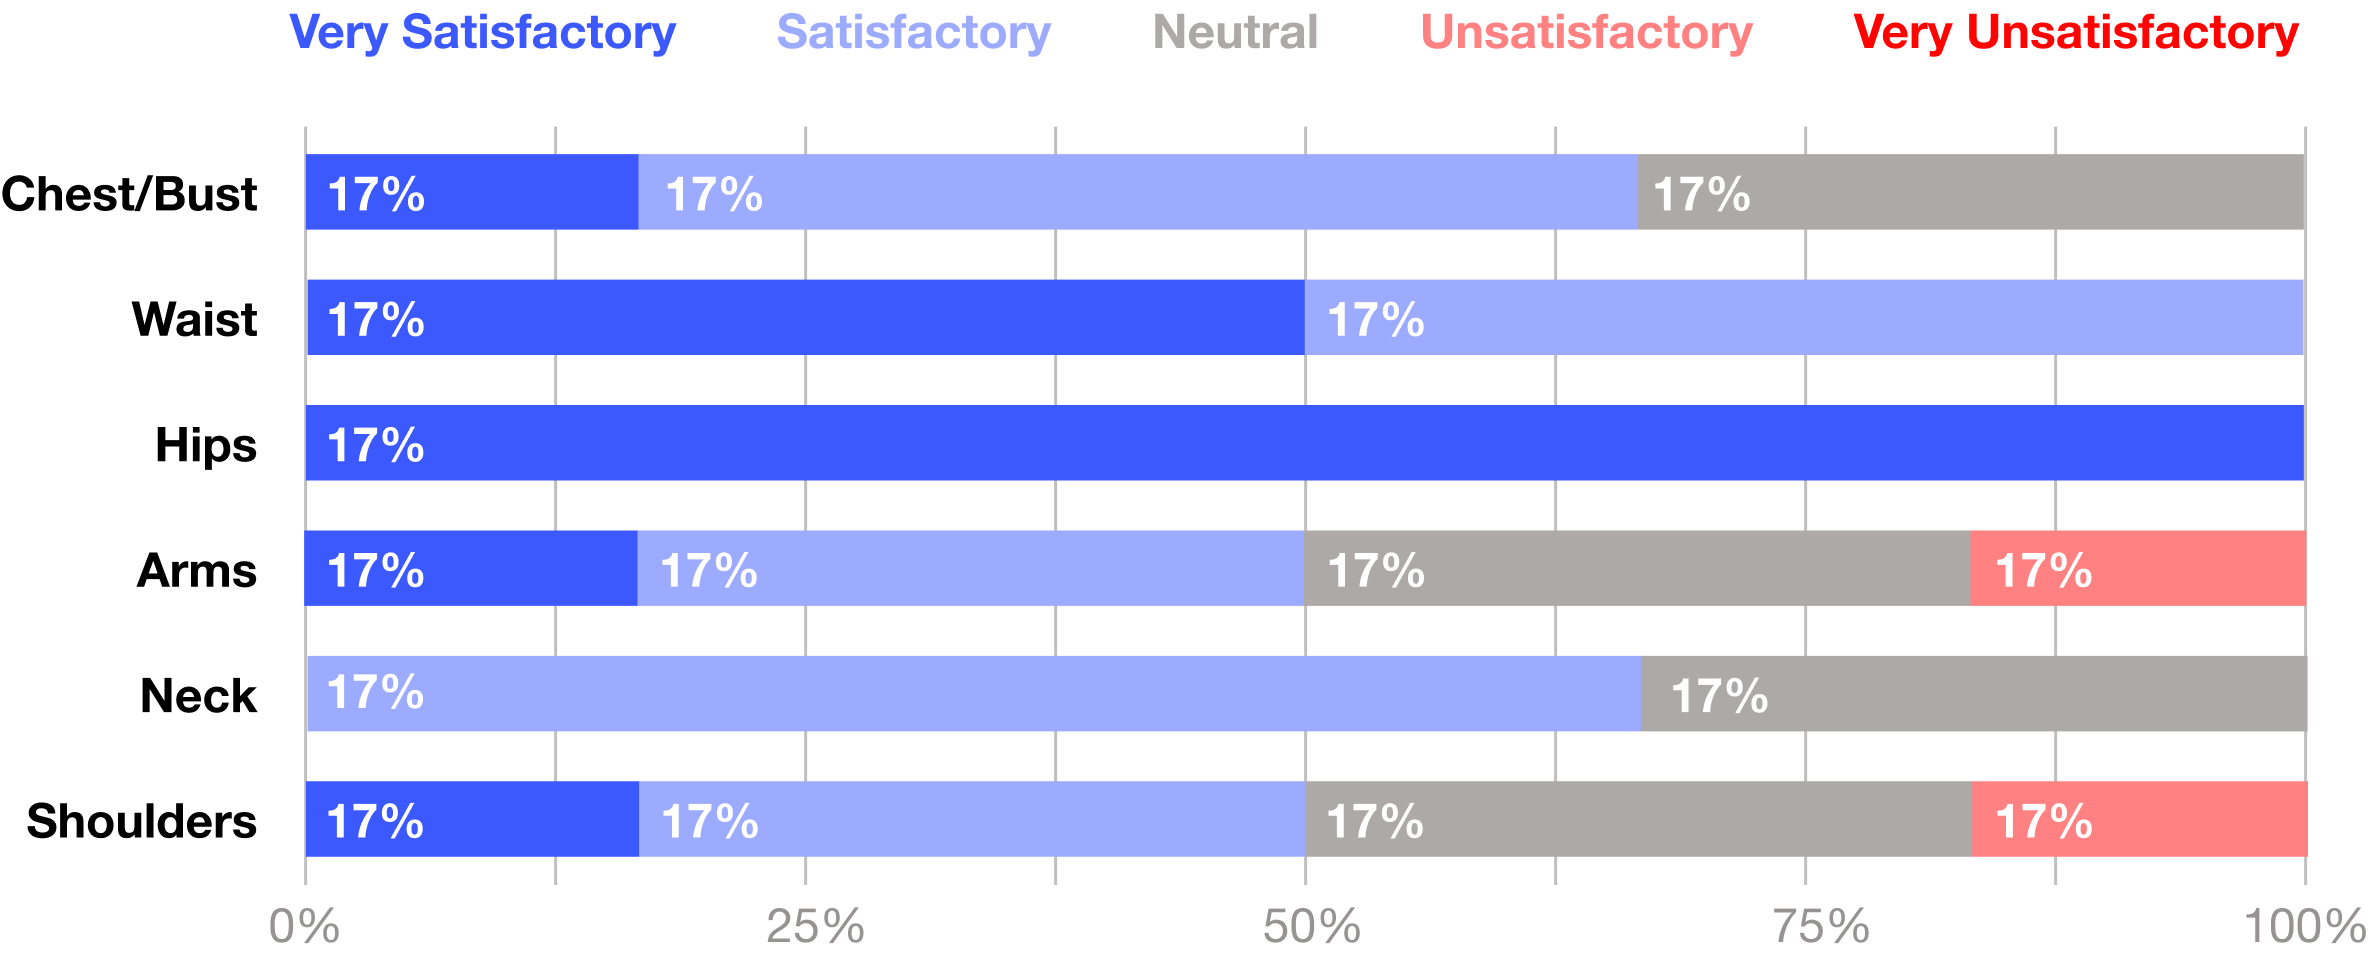
\includegraphics[width = 0.8\textwidth]{Images/comfort likert stacked bar.png}
    \caption{Comfort Likert Scales}
\end{figure}


\begin{figure}[H]
    \centering
    \begin{subfigure}[b]{0.45\textwidth}
        \centering
        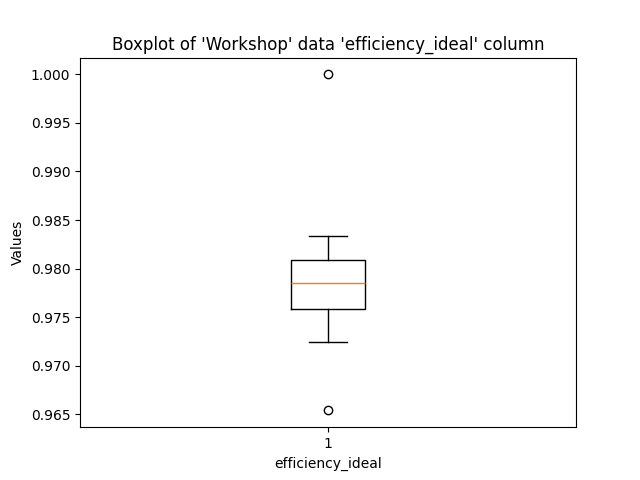
\includegraphics[width=\textwidth]{Images/Workshop_efficiency_ideal_Boxplot.png}
        \caption{}
    \end{subfigure}
    \hfill
    \begin{subfigure}[b]{0.45\textwidth}
        \centering
        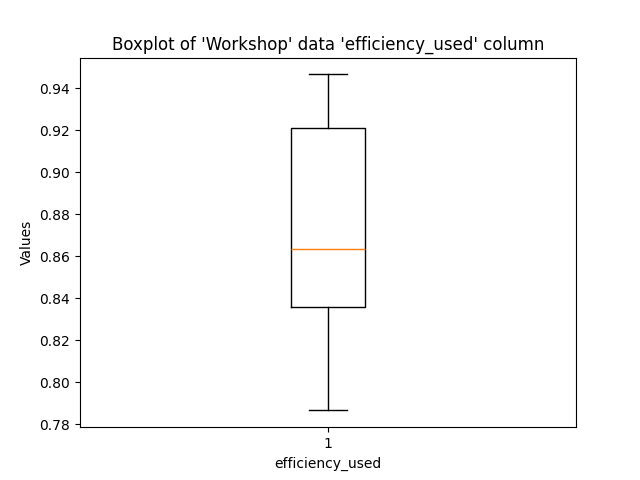
\includegraphics[width=\textwidth]{Images/Workshop_efficiency_used_Boxplot.png}
        \caption{}
    \end{subfigure}
    \caption{}
\end{figure}

\begin{figure} [H]
    \centering
    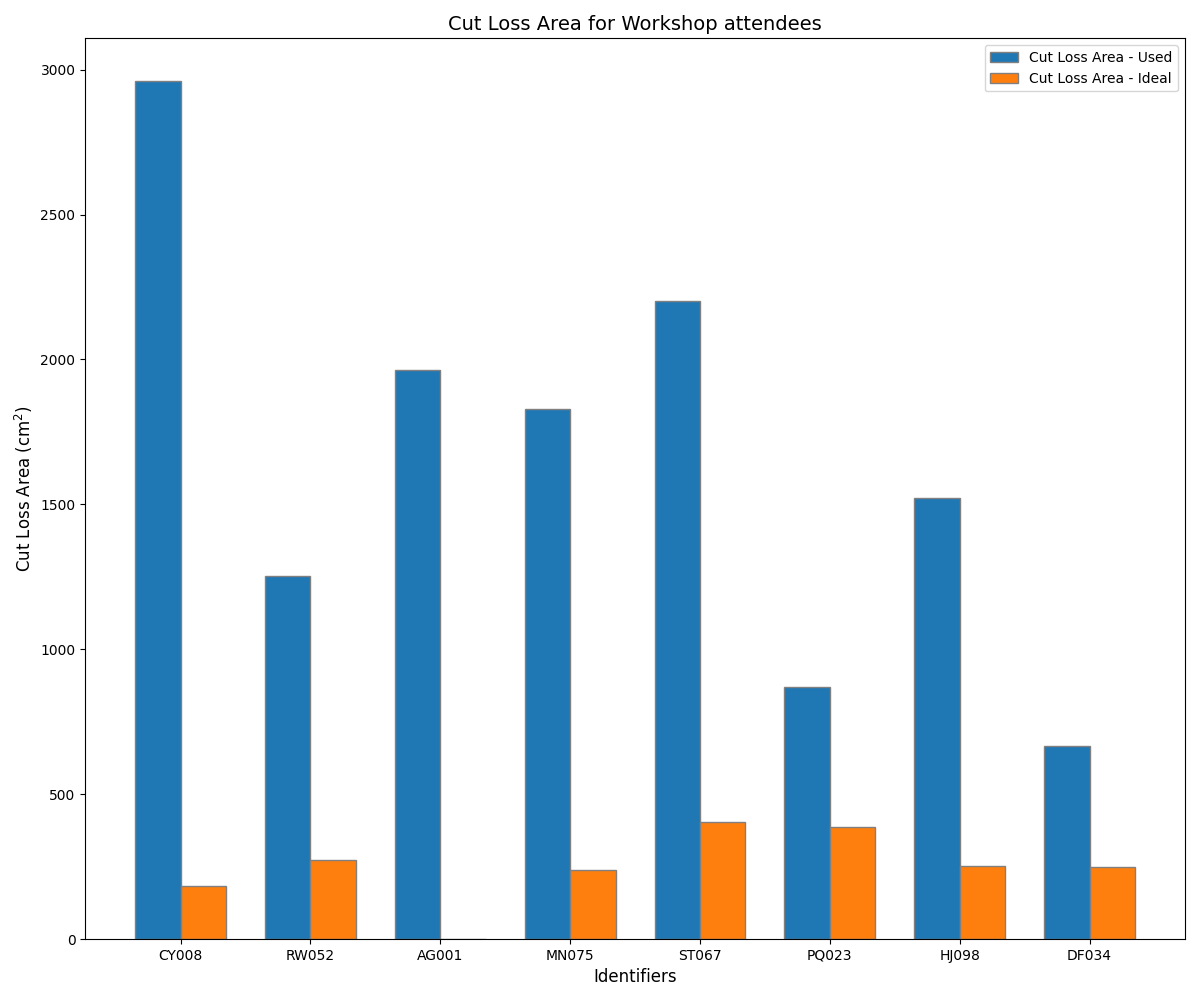
\includegraphics[width = 0.5\textwidth]{Images/Workshop_CutLossArea_Bar.png}
    \caption{Workshop Cut Loss Area}
\end{figure}
\begin{figure} [H]
    \centering
    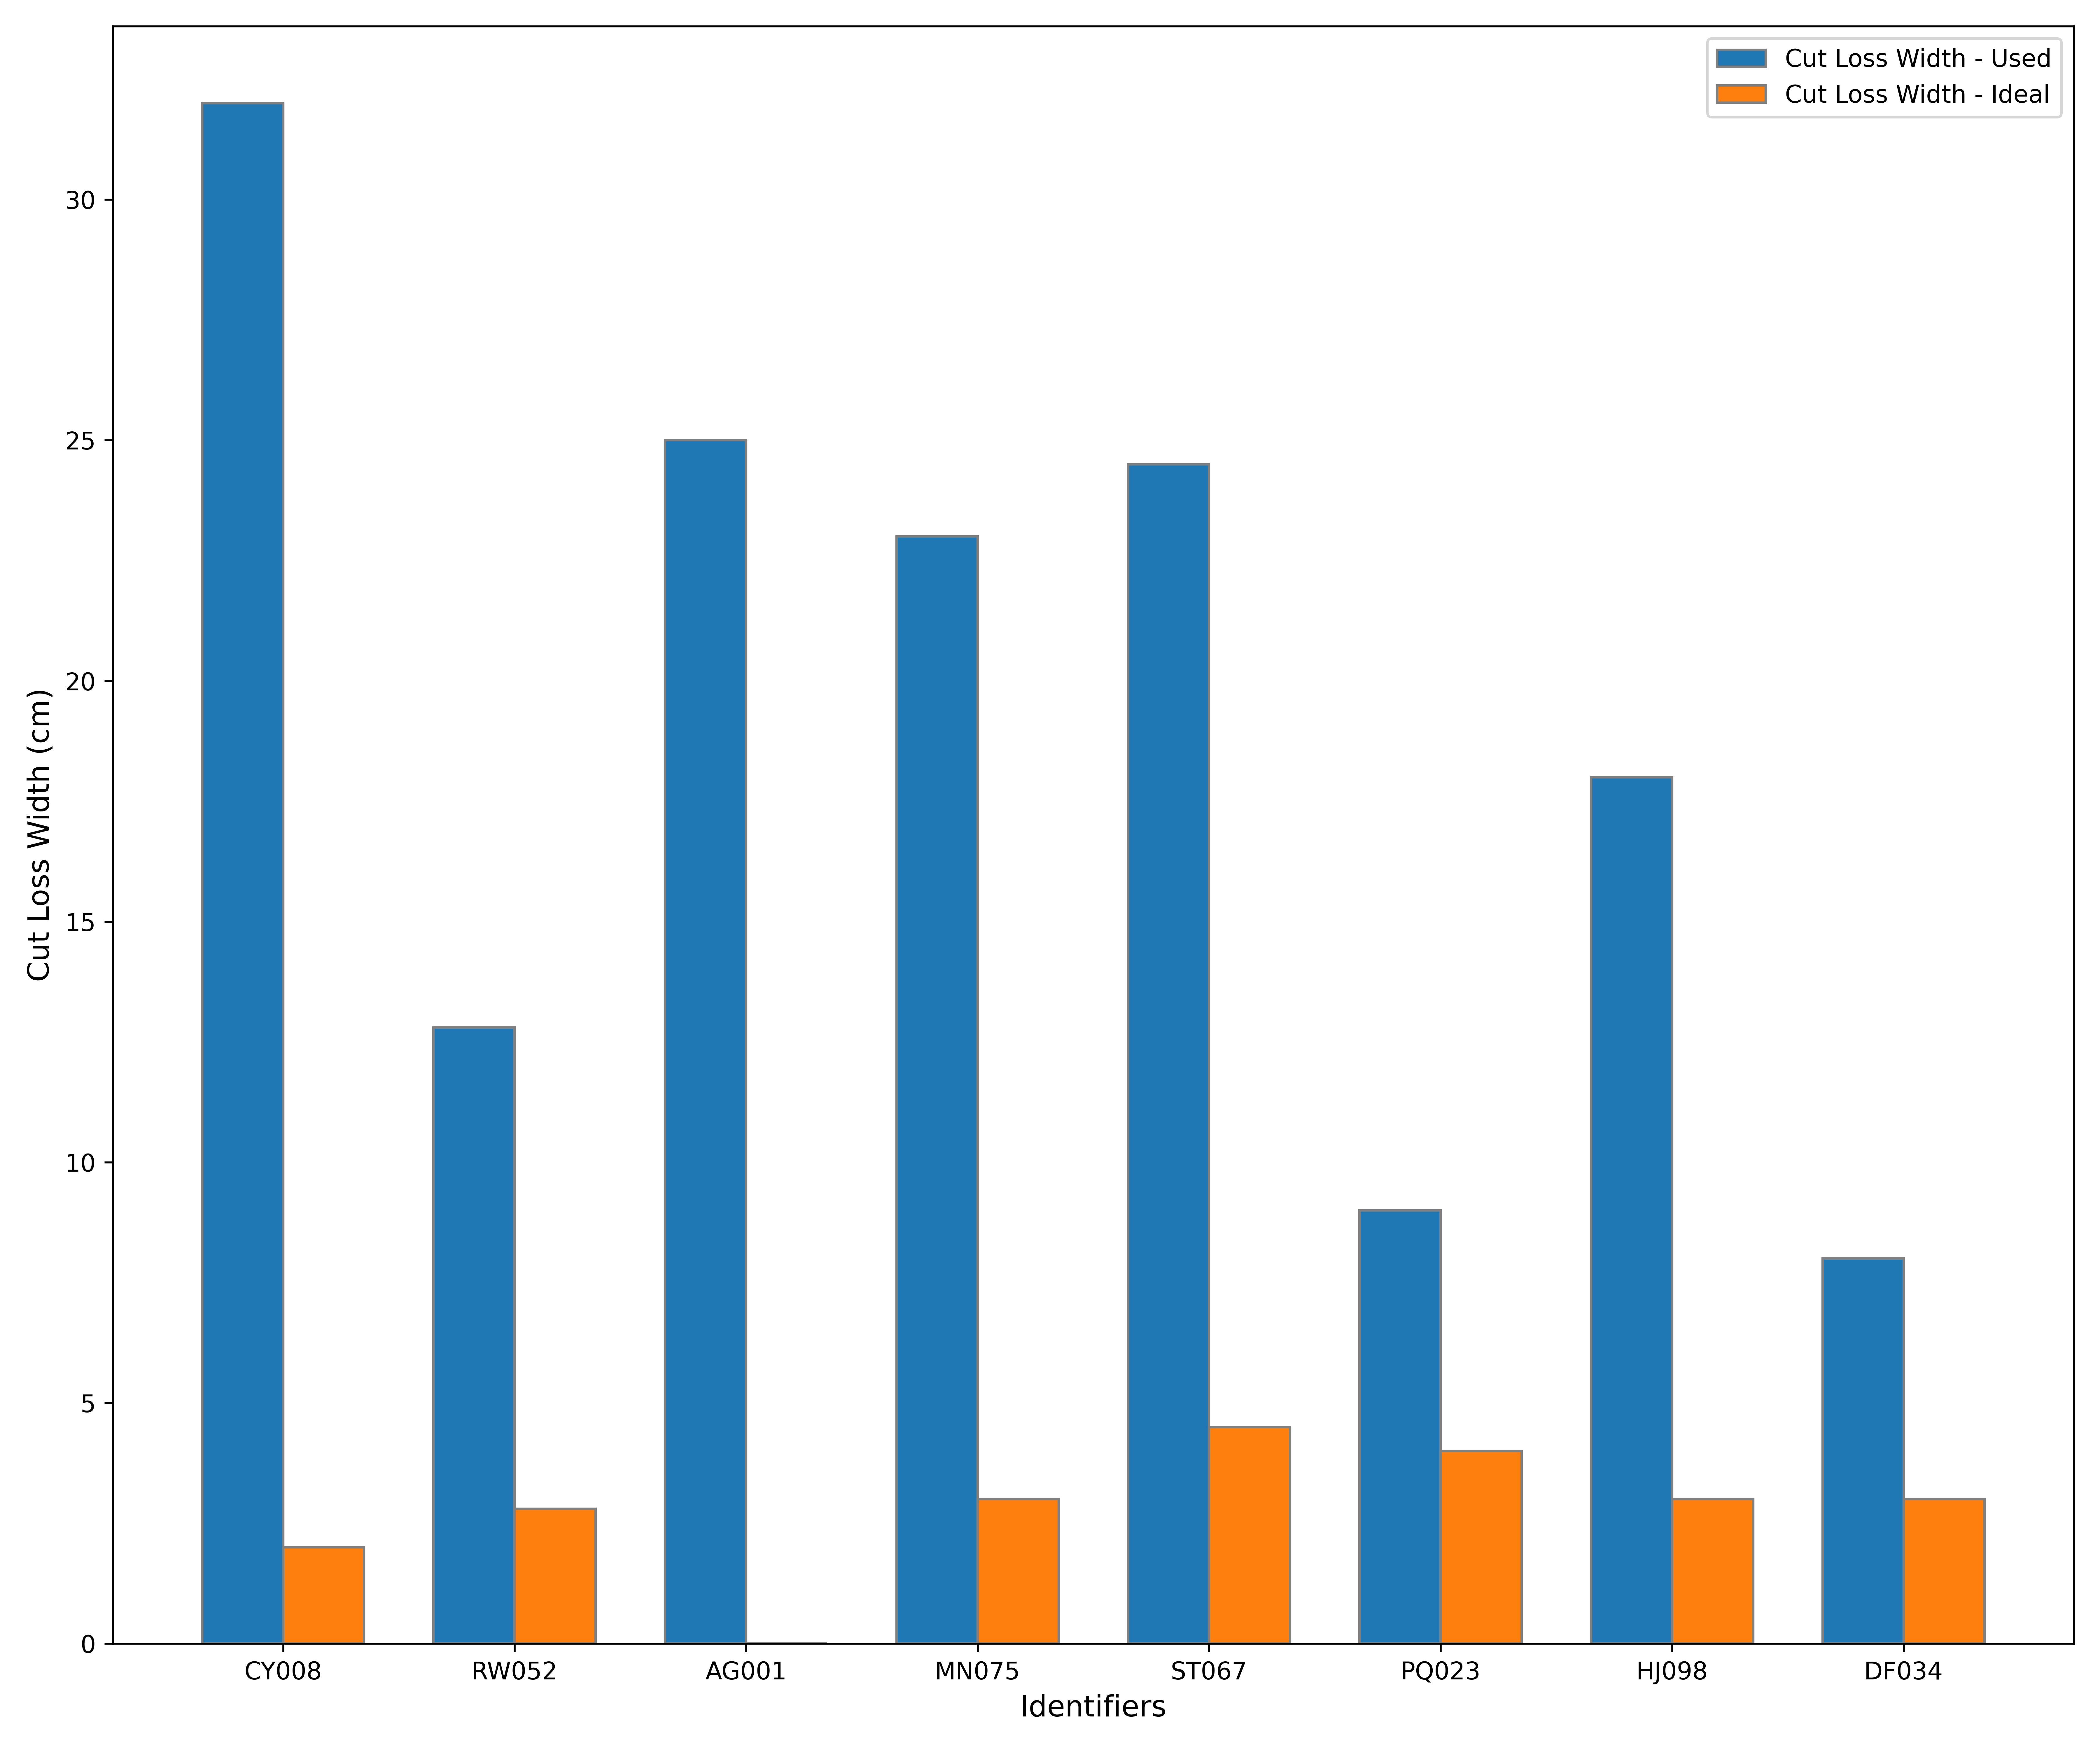
\includegraphics[width = 0.5\textwidth]{Images/Workshop_CutLossWidth_Bar.png}
    \caption{Workshop Cut Loss Width}
\end{figure}
\begin{figure} [H]
    \centering
    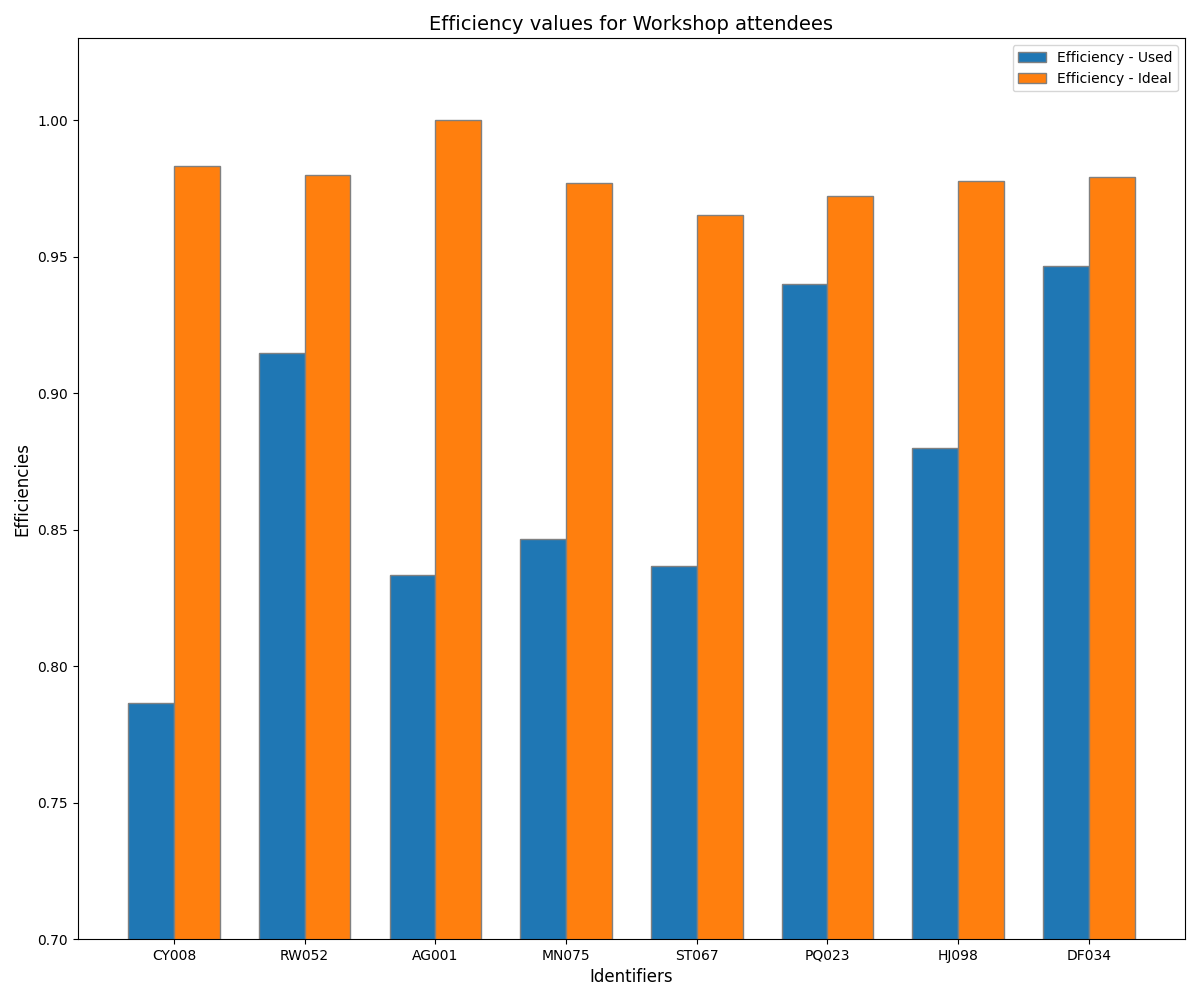
\includegraphics[width = \textwidth]{Images/Workshop_Eff_bar.png}
    \caption{Workshop Fabric Efficiency}
\end{figure}
\begin{figure} [H]
    \centering
    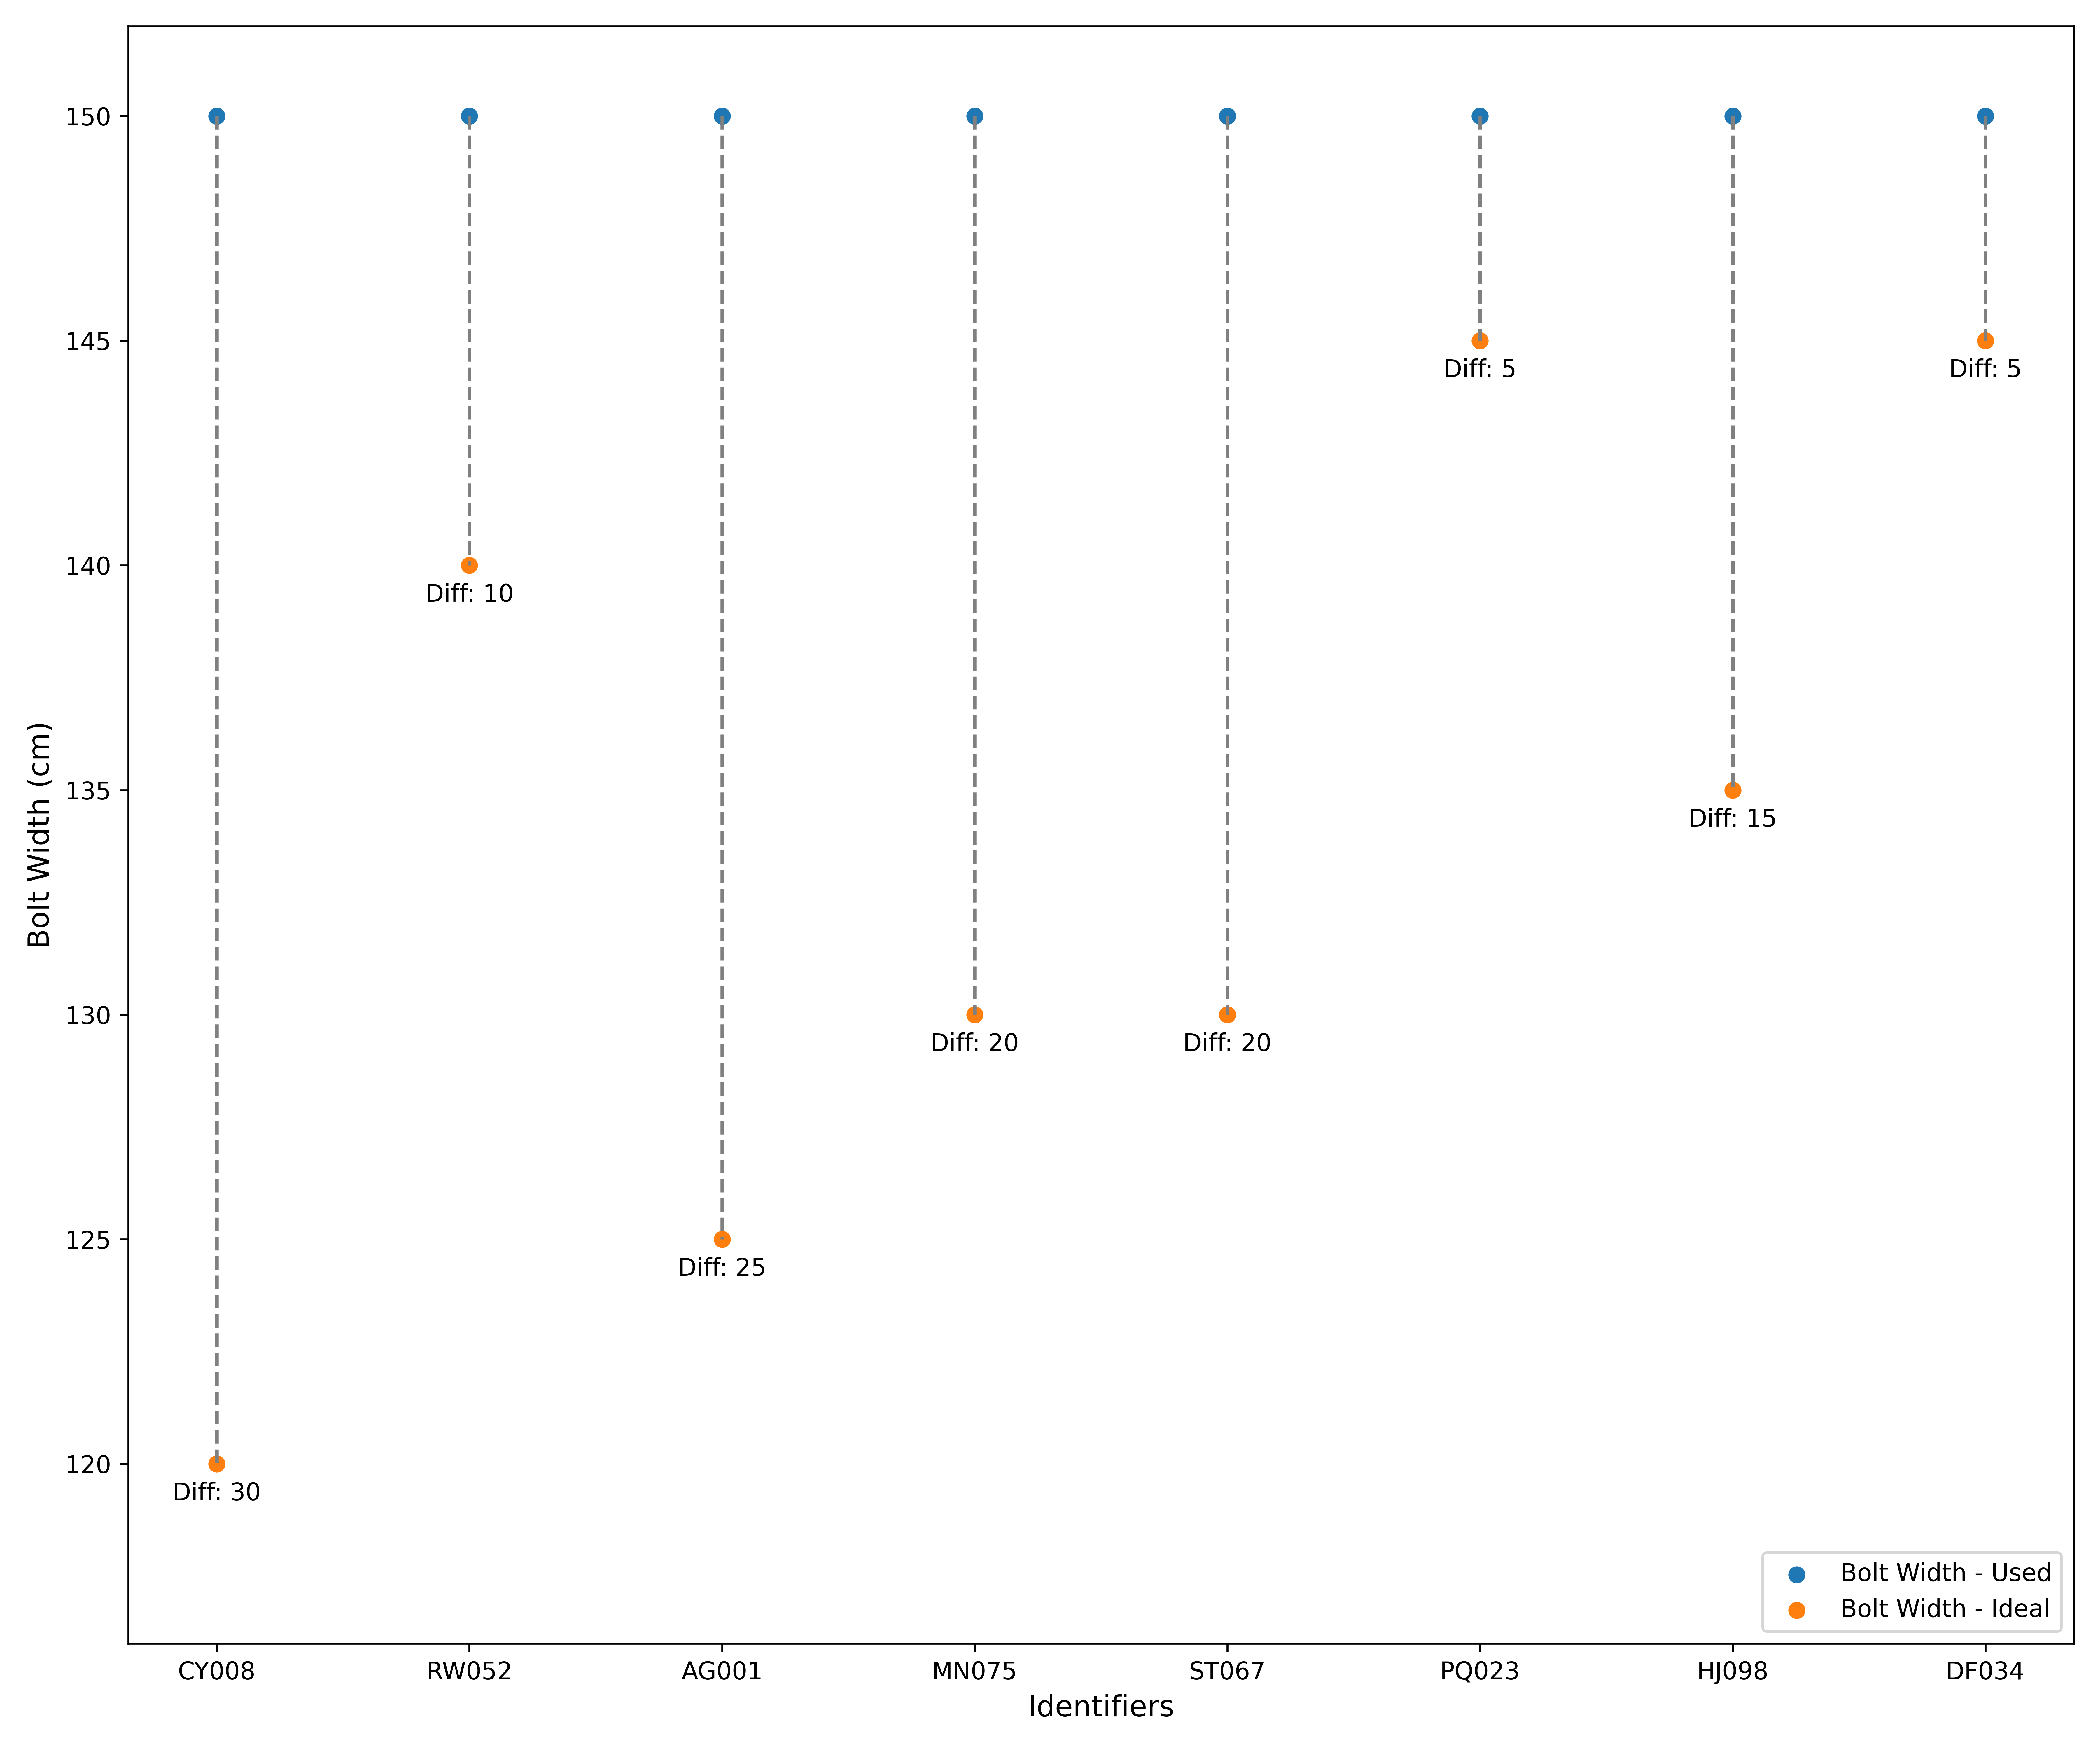
\includegraphics[width = \textwidth]{Images/Workshop_BoltWidths_Scatter.png}
    \caption{Workshop Ideal Bolts}
\end{figure}

Efficiency, bolt width, cut loss width, and cut loss area for Workshop Study comparing ideal bolt and actual used bolt. All efficiencies when using ideal bolt width are greater than 95\%.


\section{Body Scans Study}

The median is a measure of central tendency that is less affected by extreme values than the mean so should use that when many outliers present ???

\subsection{Distibutions}
Body Scans Study have a mean maximum bodice circumferemce of 99.58 cm, median of 98.25 cm and a standard deviation of 8.61 cm. The mean and median are close, indicating a relatively symmetrical distribution with a slight skew towards larger values. There is moderate variability (standard deviation of 8.613), with some outliers above 110 cm.

The mean shirt length is 62.40 cm, median of 64.5 cm, and a standard deviation of 6.72 cm. 

\begin{figure}[htb]
    \centering
    \begin{subfigure}[b]{0.45\textwidth}
        \centering
        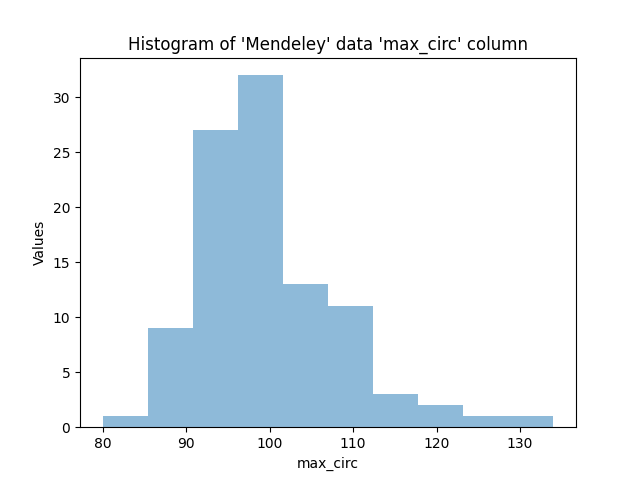
\includegraphics[width=\textwidth]{Images/Mendeley_max_circ_Hist.png}
        \caption{Histogram}
    \end{subfigure}
    \hfill
    \begin{subfigure}[b]{0.45\textwidth}
        \centering
        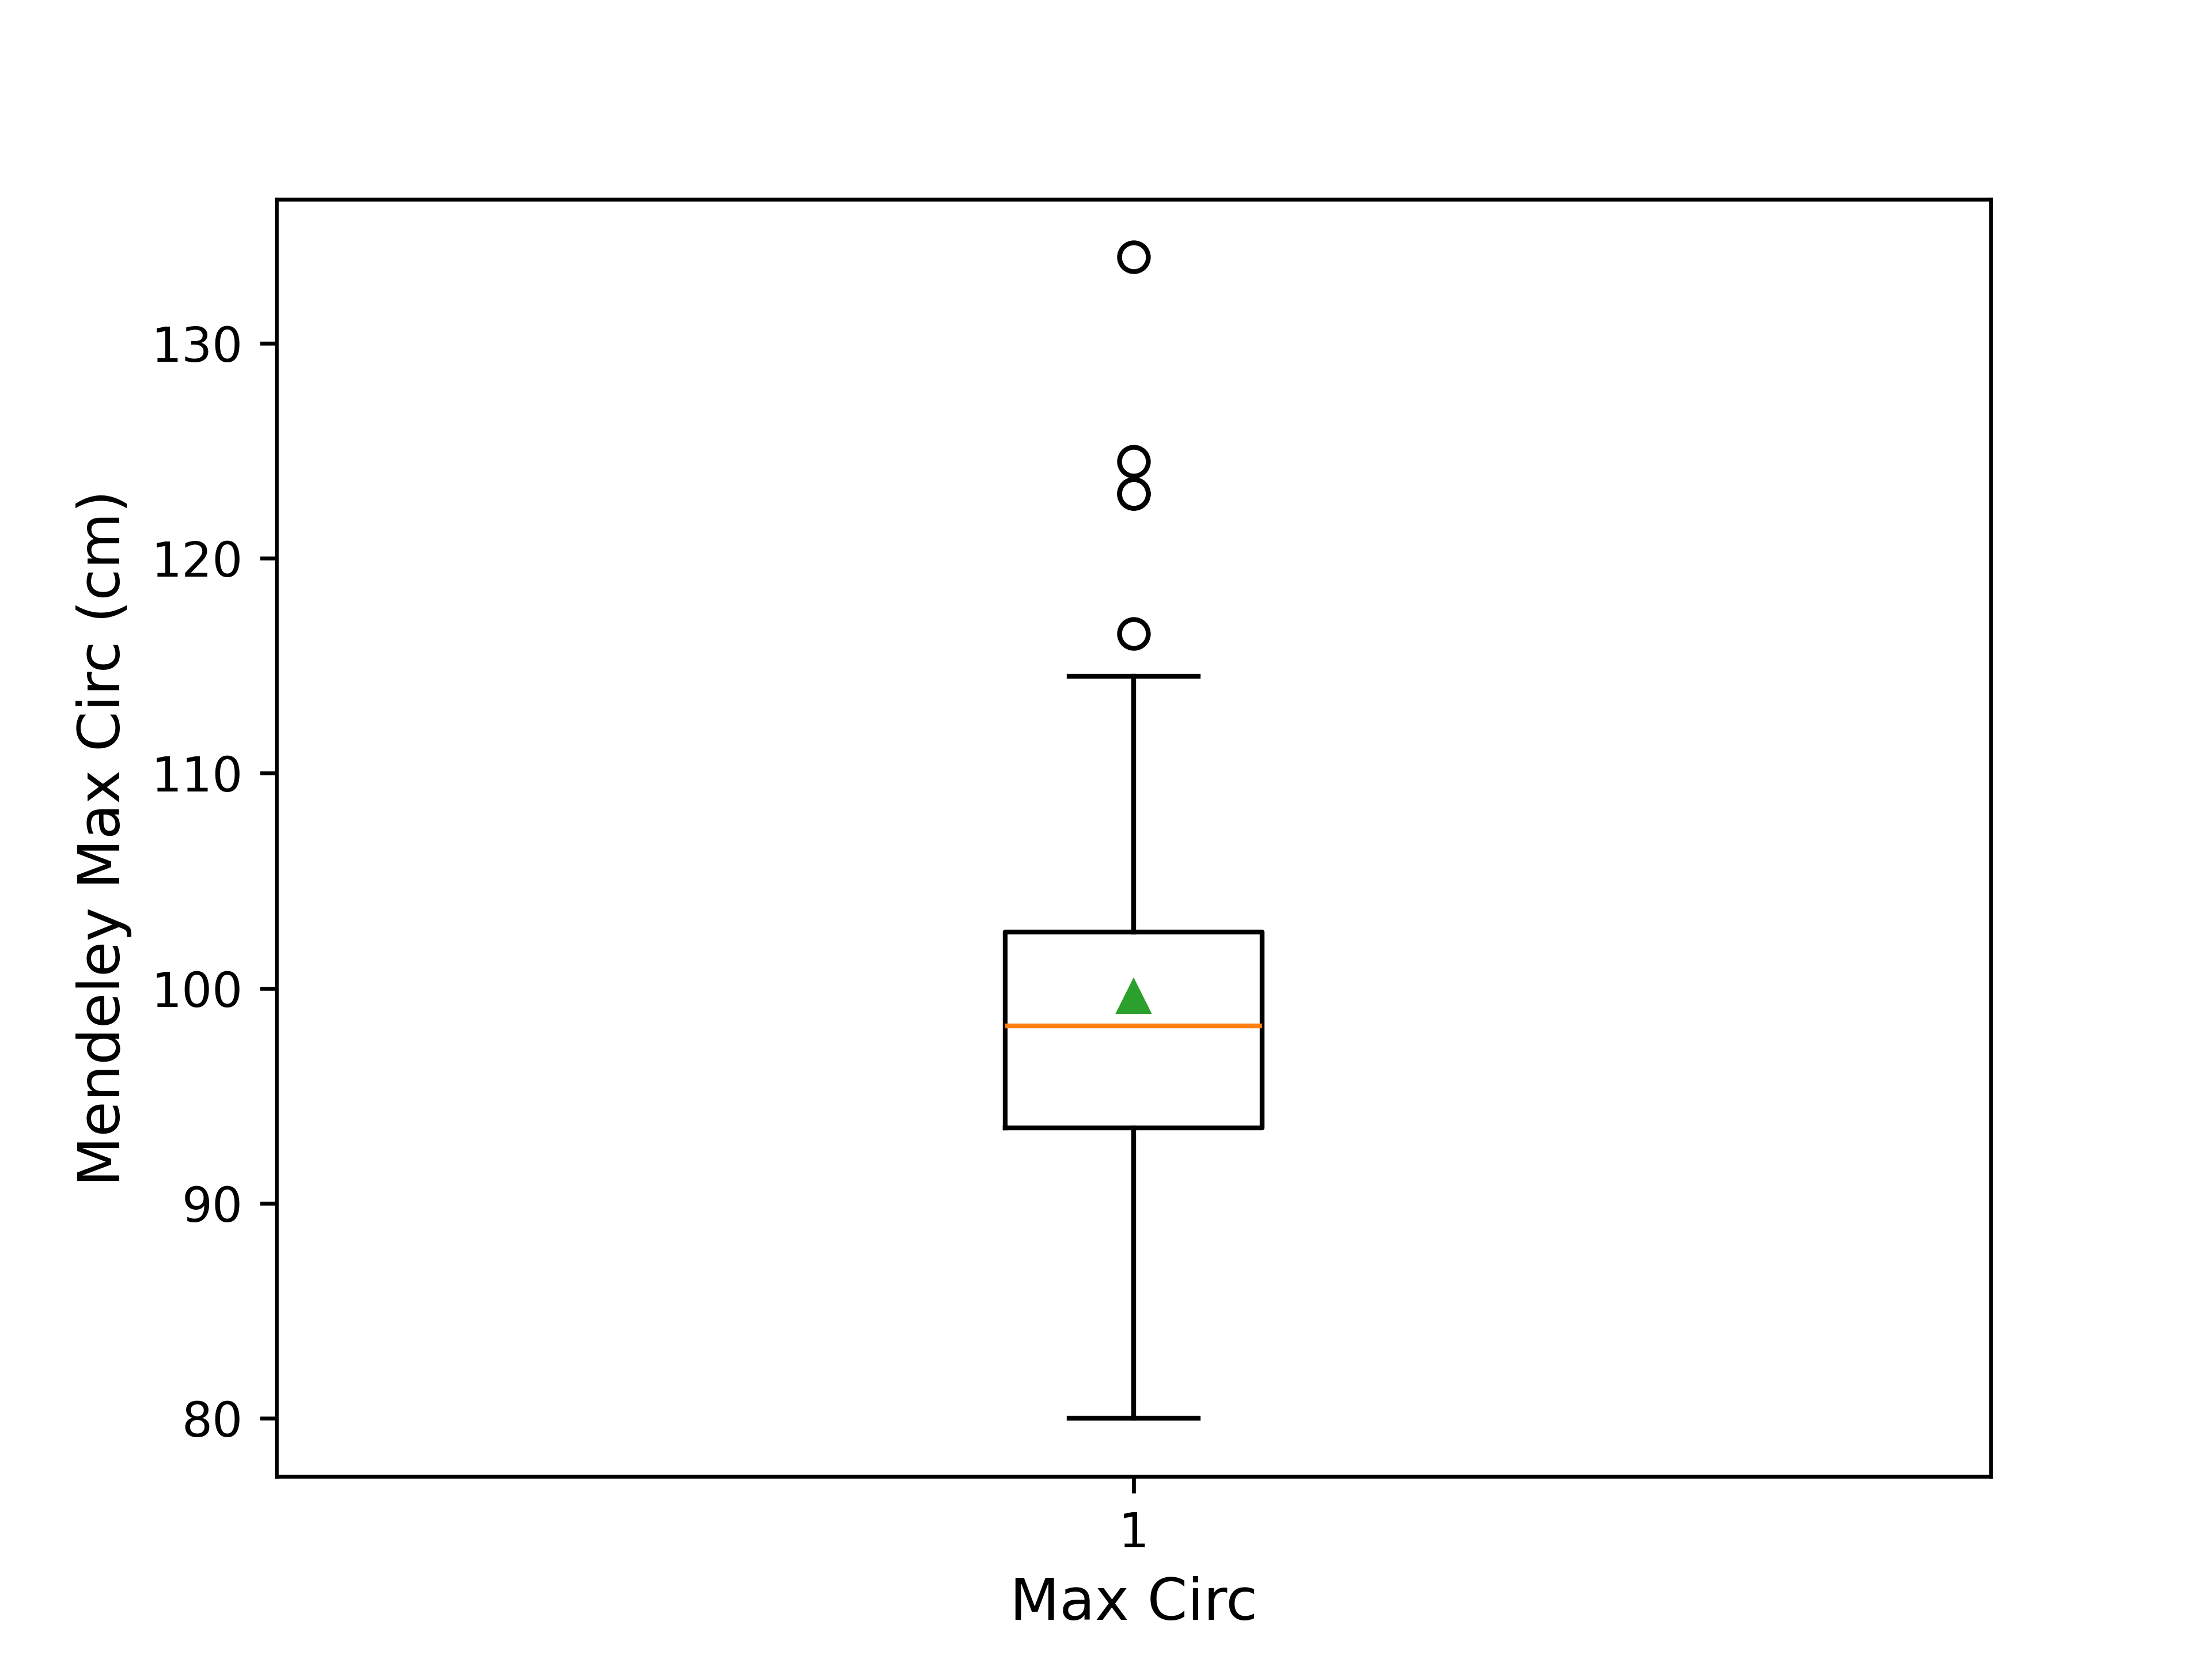
\includegraphics[width=\textwidth]{Images/Mendeley_max_circ_Boxplot.png}
        \caption{Boxplot}
    \end{subfigure}
    \caption{Distribution of max bodice circumference for Body Scans Study}
\end{figure}

\begin{figure}[htb]
    \centering
    \begin{subfigure}[b]{0.45\textwidth}
        \centering
        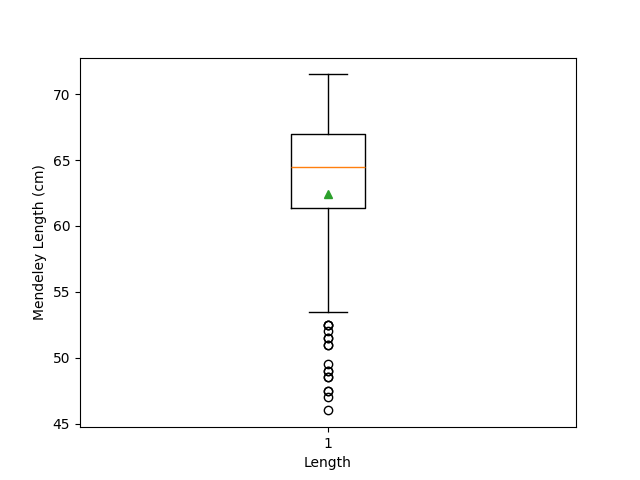
\includegraphics[width=\textwidth]{Images/Mendeley_shirt_length_Boxplot.png}
        \caption{Histogram}
    \end{subfigure}
    \hfill
    \begin{subfigure}[b]{0.45\textwidth}
        \centering
        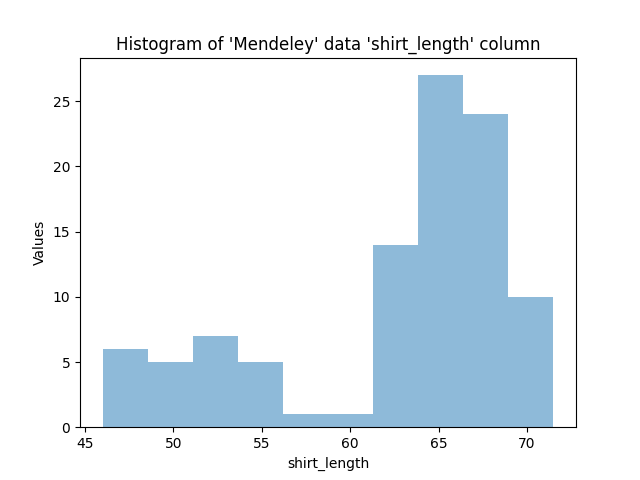
\includegraphics[width=\textwidth]{Images/Mendeley_shirt_length_Hist.png}
        \caption{Boxplot}
    \end{subfigure}
    \caption{Distribution of calculated shirt length for Body Scans Study}
\end{figure}

\subsubsection{Fabric Use}
Efficiency, bolt width, cut loss width, and cut loss area for 100 scans study comparing ideal bolt and hypothetical used bolt.
When using the ideal bolt width, the mean efficiency is 98\%, median efficiency is 98\%, and the standard deviation is 1\%. The mean ideal bolt width is 133 cm and median ideal bolt is 130 cm.
\begin{figure} [H]
    \centering
    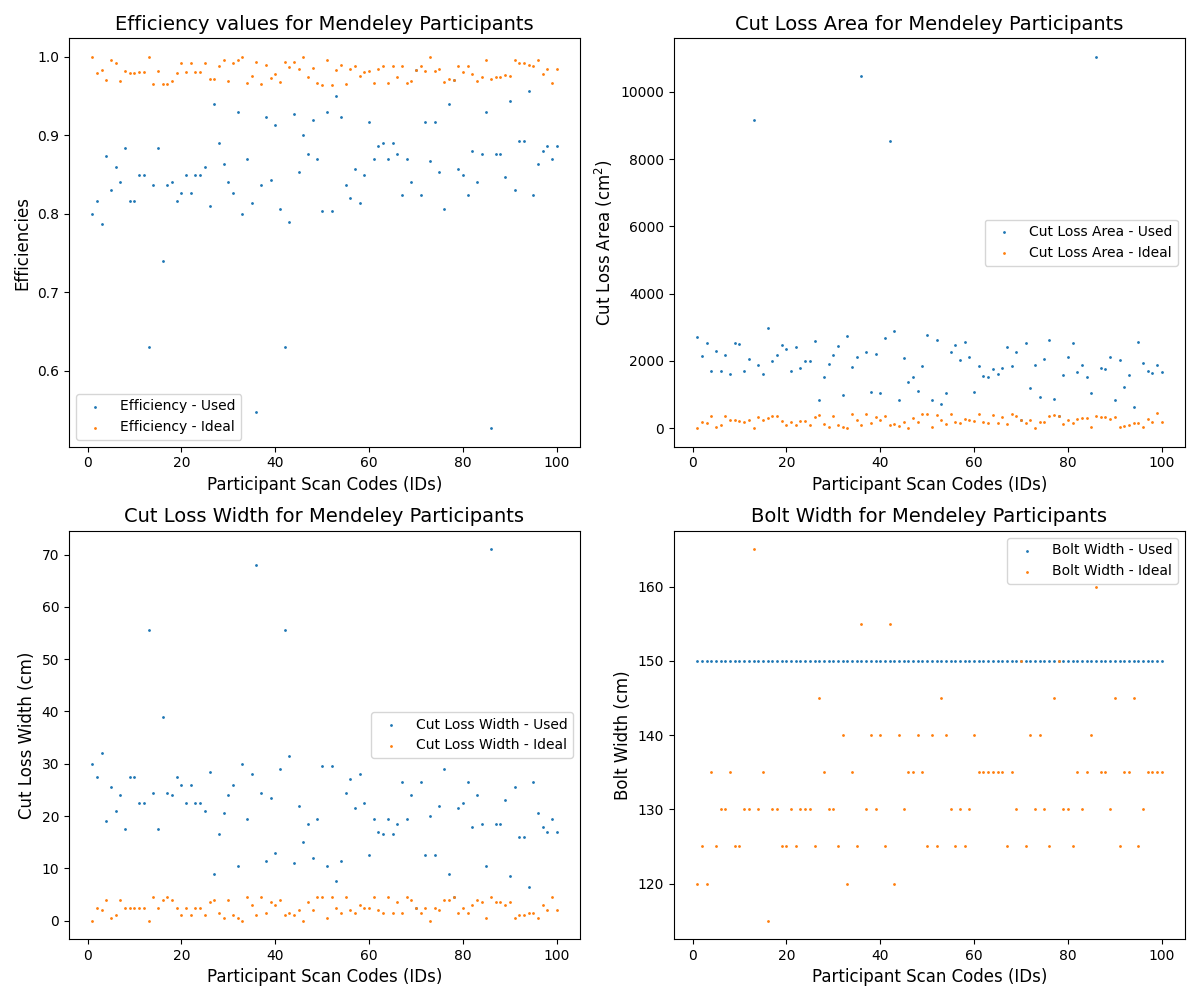
\includegraphics[width = \textwidth]{Images/Mendeley_Plot.png} 
    \caption{Used and Ideal Efficiency Metrics for 100 Scans Study}
\end{figure}

Cohort analysis
\begin{table} [H]
    \centering
    \begin{tabular}{p{2cm}|p{2cm}|p{2cm}|p{2cm}|p{2cm}|p{2cm}|p{2cm}}
        \textbf{Bolt Width} & \textbf{Mean Eff} & \textbf{Median Eff} & \textbf{St Dev Eff} & \textbf{Mean Loss Area} & \textbf{Median Loss Area} & \textbf{St Dev Loss Area}\\
        \hline % this produces a horizontal line, this could be used elsewhere in the table
        110& 81.7\% & 83.6\% & 6.1\% & 2620.64 & 2318.0 & 889.32\\
        115& 78.5\% & 80.0\% & 6.0\% & 3233.87 & 2922.75 & 937.46\\
        120& 76.2\% & 77.1\% & 7.4\% & 3737.44 & 3556.88 & 1207.17\\
        125& 78.7\% & 75.6\% & 12.1\% & 3526.84 & 4025.0 & 2097.15\\
        130& 83.7\% & 91.7\% & 13.5\% & 2771.99 & 934.5 & 2542.75\\
        135& 87.9\% & 92.9\% & 12.3\% & 1997.82 & 843.0 & 2501.29\\
        140& 88.8\% & 91.1\% & 9.2\% & 1716.44 & 1131.0 & 2025.64\\
        145& 87.3\% & 88.1\% & 8.1\% & 1865.09 & 1491.63 & 1849.15\\
        150& 85.2\% & 85.5\% & 7.1\% & 2158.84 & 1890.75 & 1679.22\\
        155& 83.3\% & 83.1\% & 6.2\% & 2418.42 & 2333.63 & 1388.62\\
        160& 81.2\% & 80.6\% & 5.4\% & 2752.84 & 2795.13 & 1076.74\\
        165& 79.1\% & 78.3\% & 5.2\% & 3089.52 & 3250.13 & 782.20\\
        \end{tabular}
    \caption{Description of Cohort Analysis on Different Bolts for 100 Scans Study}
\end{table}
\textbf{SHOULD CHANGE FORMAT OF GRAPHS BELOW BECAUSE NOT CONTINOUS???}
\begin{figure}[H]
    \centering
    \begin{subfigure}[b]{0.45\textwidth}
        \centering
        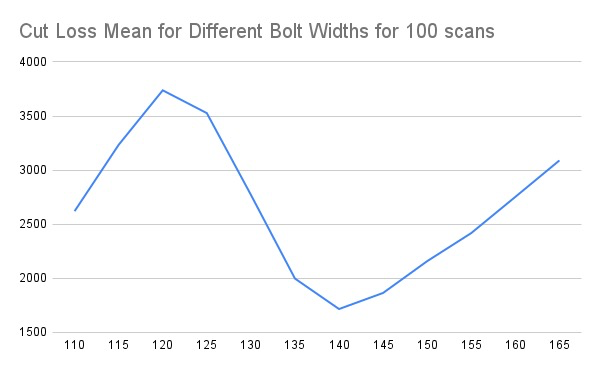
\includegraphics[width=\textwidth]{Images/Cut Loss Mean for Different Bolt Widths for 100 scans.png}
        \caption{Cut Loss Area}
    \end{subfigure}
    \hfill
    \begin{subfigure}[b]{0.45\textwidth}
        \centering
        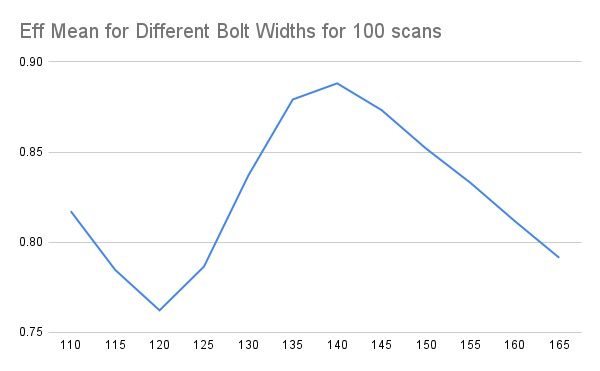
\includegraphics[width=\textwidth]{Images/Eff Mean for Different Bolt Widths for 100 scans.png}
        \caption{Efficiency}
    \end{subfigure}
    \caption{Mean Cut Loss Area Used and Efficiency Used for Different Bolt Widths for 100 Scans Study}
\end{figure}

For this cohort, using a 140 cm wide fabric bolt minimises the cut loss area and maximises the efficiency.

Count of pattern orientation on starting fabric and possibility of embellishment potential for various bolt widths ranging from 110 to 160 cm.
\begin{figure} [H]
    \centering
    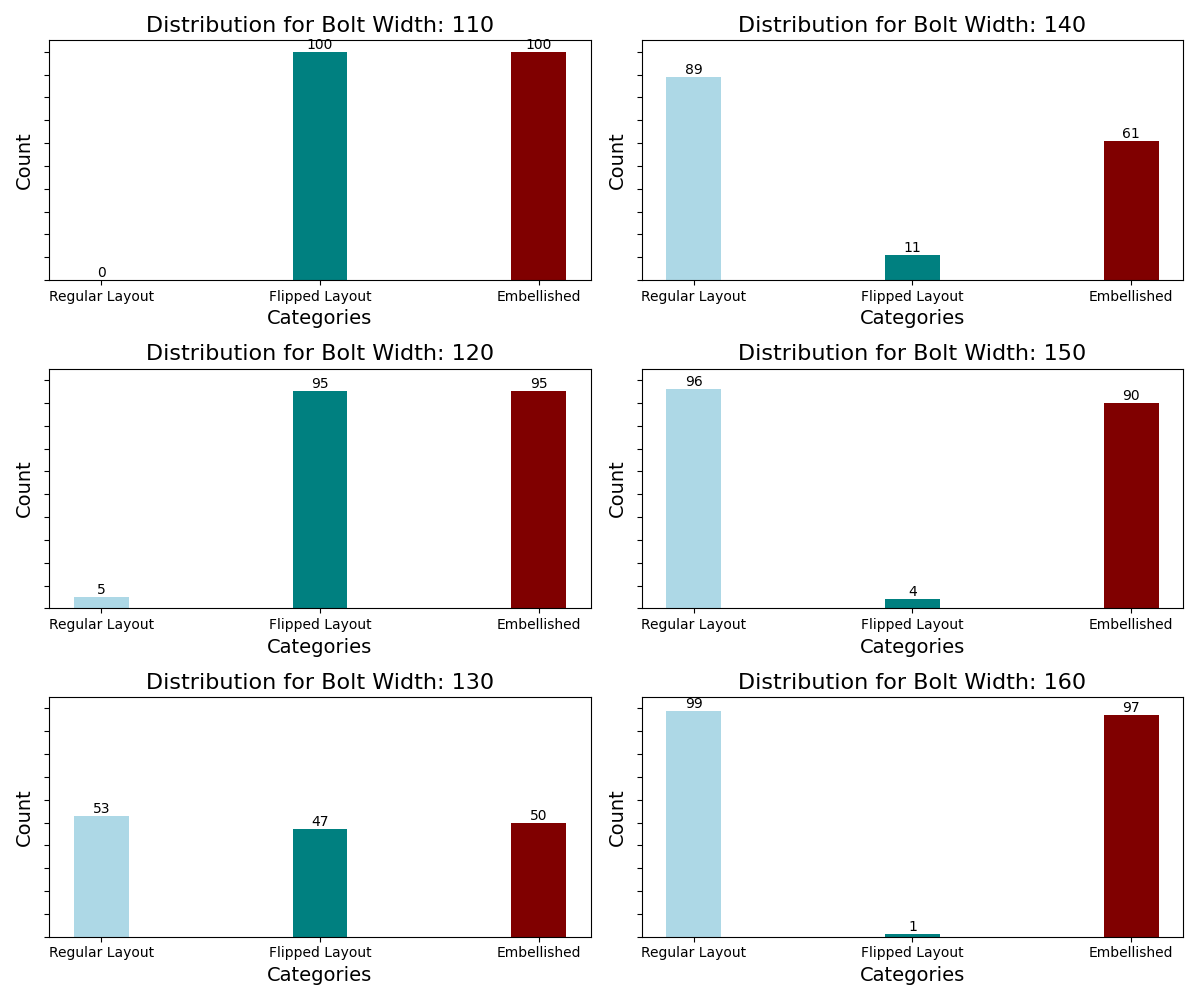
\includegraphics[width = \textwidth]{Images/Mendeley_Bar.png}
    \caption{Layout and Embellishment Possibility for 100 Scans Study}
\end{figure}
For the range of bolt widths between 110 and 160 cm, each pattern generated for the Mendeley dataset participants will fit in the regular or rotated orientation. No mitigation strategies need to be employed within this range of bolts.

\textbf{ADD recoup of cut loss area due to embellishment}

\section{Personal Case Study}


\chapter{Discussion}


\section{Method Limitations} \label{sec:sections}

One notable limitation is the reliance on accurate body measurements to achieve a customisable fit. Manual measurements can introduce human error, while technological solutions such as body scanners may not be universally accessible or affordable for all domestic sewers.

\section{Data Limitations}
The data collected for this project primarily involves body measurements and user feedback on fit and fabric utilization. One significant limitation is the sample size, which may not be large enough to capture the full variability in body shapes and sizes. A larger, more diverse sample would provide more comprehensive insights into how well the parameterized pattern accommodates different body types. However we have to make the compromise here given the project timeline and available resources. Additionally, the project relies on self-reported data, which can be subject to biases and inaccuracies. For instance, participants’ subjective assessments of fit and comfort may vary based on personal preferences and experiences. 

The data on fabric utilization also presents limitations. Tthe efficiency of fabric utilization is measured under controlled conditions, which may not accurately reflect real-world sewing practices where additional waste can occur. And creativity of the fashion designer can lead to more complex and intuitive uses for cut loss rather than the predefined embellishment check, for a given random cut loss dimension and area.

We also have to consider the limitation arising from how the data is collected, there is difference between the methods of obtaining measurements, and not all parameterisation methods work the same because of differing measurements used in the workshop vs scan data. It may not be appropriate to always compare them because for more proper comparative analysis we would need 


\subsection{Workshop Study}
\subsection{Limited Sample Size}
Limited Data
Due to time commitments and resource constraints there were only 8 participants in the workshop. Of these, only 6 finished making the garment. Thus the data set is very limited and not amenable to sophisticated statistical analysis. Regardless, findings are presented with that caveat.
\subsubsection{Sewing Inconsistency}

Each participant sewed their own garments. There was variability in their ability and the tailoring / sewing was not held constant across all garments. This ability did affect the fit, finish, and comfort values and was not an equitable comparison of the pattern per se but the skill of the participant.

\section{Framework Limitations}

The service provided by this project, which includes the parameterized zero-waste pattern and guidance on fabric utilization, has inherent limitations. One key limitation is the dependency on users’ willingness and ability to adopt new techniques. Domestic sewers accustomed to traditional pattern-making methods may find it challenging to transition to zero-waste designs, especially if they lack prior experience with digital tools or sustainable practices.

Limitations with CLO
Posture mode is quite static in CLO and does not allow for varied postures
So we are simulating the fit in many different natural poses
Does not give much more than a static visual representation of fit

Finally, the scalability of the service presents a challenge. While the project aims to provide a practical solution for domestic sewers, the success of the parameterized pattern depends on individual users’ skills and resources. The variability in sewing experience and access to advanced tools can affect the consistency and quality of the outcomes, potentially limiting the service’s effectiveness and reach to a much wider audience.

\section{Further Work} \label{sec:sections}

\subsection{Parameterisation Tuning}
Some of the pieces in the pattern are kept constant (collar) or dictated by a specified template size (neck facing, sleevehead curve). To provide end users with more options to customise these pieces based on their body measurements or personalise aspects of the garment, the geometry of these pieces should be able to be chosen by user on input. For example, the neck facing piece geometry can be influenced by the person's neck measurement and the collar thickness and length be a personal choice. Because there are so many dependencies of other pieces on the overall ease and fit, these were not explored during this phase of Tail0r's development. Allowing user's to customise and personalise further while still maintaining the garment style will require extensive testing and tuning of parameters. It is certainly something to be explored in Tail0r's development.

\subsection{Scalability}
While the chosen short-sleeved collared shirt block serves as a useful case study, the results may not be directly applicable to other garment types with different structural and fit requirements. This specificity limits the generalisability of the findings to other types of zero-waste garments. However, it is reasonably feasible to develop an arsenal of garments using this framework with the bulk of work initially in defining and calculating parameterisation unique to the a specific pattern. To build new zero waste pattern designs and garment design, a modular approach of scalable pattern pieces would be more intuitive akin to that of GarmentCode, but this is outscope of parameterising existing patterns and rather is for developing novel designs.

\subsection{Pipeline Automation}
The manual work required to achieve the rendered garment draped on an avatar is a hindrance to the pipeline's automation. Developing a method to assign sewing lines before file import into CLO 3D would greatly speed up this process and forego need of the user to be skilled in CLO 3D. Being able to quickly show the user a visual of the final garment within minutes of entering their inputs would be invaluable in developing this framework into an accessible product. This could involve building a render environment within Tail0r, but a tradeoff has to be made on the computational intentions of Tail0r and the limitations when using third party 3D tools.

\subsection{UI}
Finally, creating a simple UI where the user can type in their measurements and preferences would go a long way in making this technology more accessible and usable. Though the GitHub repo of this technology is available online, end user would have to know how to run and enter inputs into the command line correctly to get their bespoke pattern. Developing a UI would strength the Tail0r as a ready-to-use tool. The user can get their pattern and instructions displayed on the webpage, and with more development, view the 3D render before making the choice to proceed and cut fabric from the bolt.

\section{Outcome Impact and Potential}


\chapter{Reflection}
If tight on words, Lorenzo says this content can be presented in viva rather than in report. But good to include something here if possible because markers will perform a preliminary marking before viva.
\section{Skills Development}

\section{Management}

\chapter{Conclusion}
In this project, a method for parameterizing a zero-waste pattern for a short-sleeved collared shirt was developed to address fabric waste and optimize garment fit for domestic sewers. The parameterized pattern provides end users with a choice of designs: a true zero-waste design that is fully customized and another design that minimizes waste as much as possible for an ideal bolt width. This approach acknowledges the traditional fabric waste in conventional pattern-making processes, suggests fabric cut loss utility strategies and offers practical insights for balancing fit and sustainability. The outputs of the project not only create customizable patterns but also render files that can be imported into CLO for virtual draping and visualization. This provides users with a comprehensive view of the final garment before physical production, enhancing their ability to make informed decisions about fit and fabric utilization. Workshop findings have provided proof of concept for the parameterization approach, demonstrating its feasibility and practical application. However, the fit findings need more extensive testing to be generalized further. Further physical testing should involve a larger and more diverse sample size to validate the fit and ensure the pattern’s applicability across various body types. Analysis on a publicly available dataset of scanned bodies verified pattern suitability across  efficinecy metrics, showing that custom size patterns using an ideal bolt have at least 95\% fabric use efficiency. Future enhancements could include expanding the pattern parameterisation options to accommodate a wider range of customisation to improve fit accuracy and to integrate the framework into a webtool to streamline the user experience. It is feasible to apply the methods of this framework to parameterise different pattern designs. This project represents a significant step towards sustainable fashion practices by providing valuable insights and practical tools for independent designers and domestic sewers. By offering customizable patterns with clear metrics on waste efficiency, the project empowers users to make informed choices, balancing fit and sustainability in their garment production.


\chapter*{Acknowledgements}
\addcontentsline{toc}{chapter}{Acknowledgements}
My deepest gratitude to Dr Becky Stewart for her invaluable guidance over the last two years, supporting my involvement in academic research and expanding my knowledge in textiles and fashion. Thanks to Lei Ge for early insight into zero-waste pattern theory and strategies. I am grateful to Joy Zhou and Mingke Wang for their sewing expertise and support as workshop assistants. Special thanks to Simeon Gill and the Apparel Design Engineering group at the University of Manchester for helping me understand the dataset, its applications for this project, and their support during my campus visit for a bosy scan. I would like to recognize Kamyar Hazeri for his assistance with and initial body scan using a handheld scanner. Finally, I would like to thank my family and friends for their encouragement and support throughout this project.

%%%%%%%%%%%%%%%%%%%%%%%%%%%%%%%%%%%%%%%%%%%
% MY BIBLIOGRAPHY
%%%%%%%%%%%%%%%%%%%%%%%%%%%%%%%%%%%%%%%%%%%

\bibliographystyle{ieeetr}

\bibliography{references}

%%%%%%%%%%%%%%%%%%%%%%%%%%%%%%%%%%%%%%%%%%%
% MY APPENDICES
%%%%%%%%%%%%%%%%%%%%%%%%%%%%%%%%%%%%%%%%%%%
\appendix

%\chapter{An example of an appendix}
This is what an appendix looks like!

% \label{sec:session}
\chapter{Session Protocol}
%% This shows appendix shows how to attach a file to the appendix.
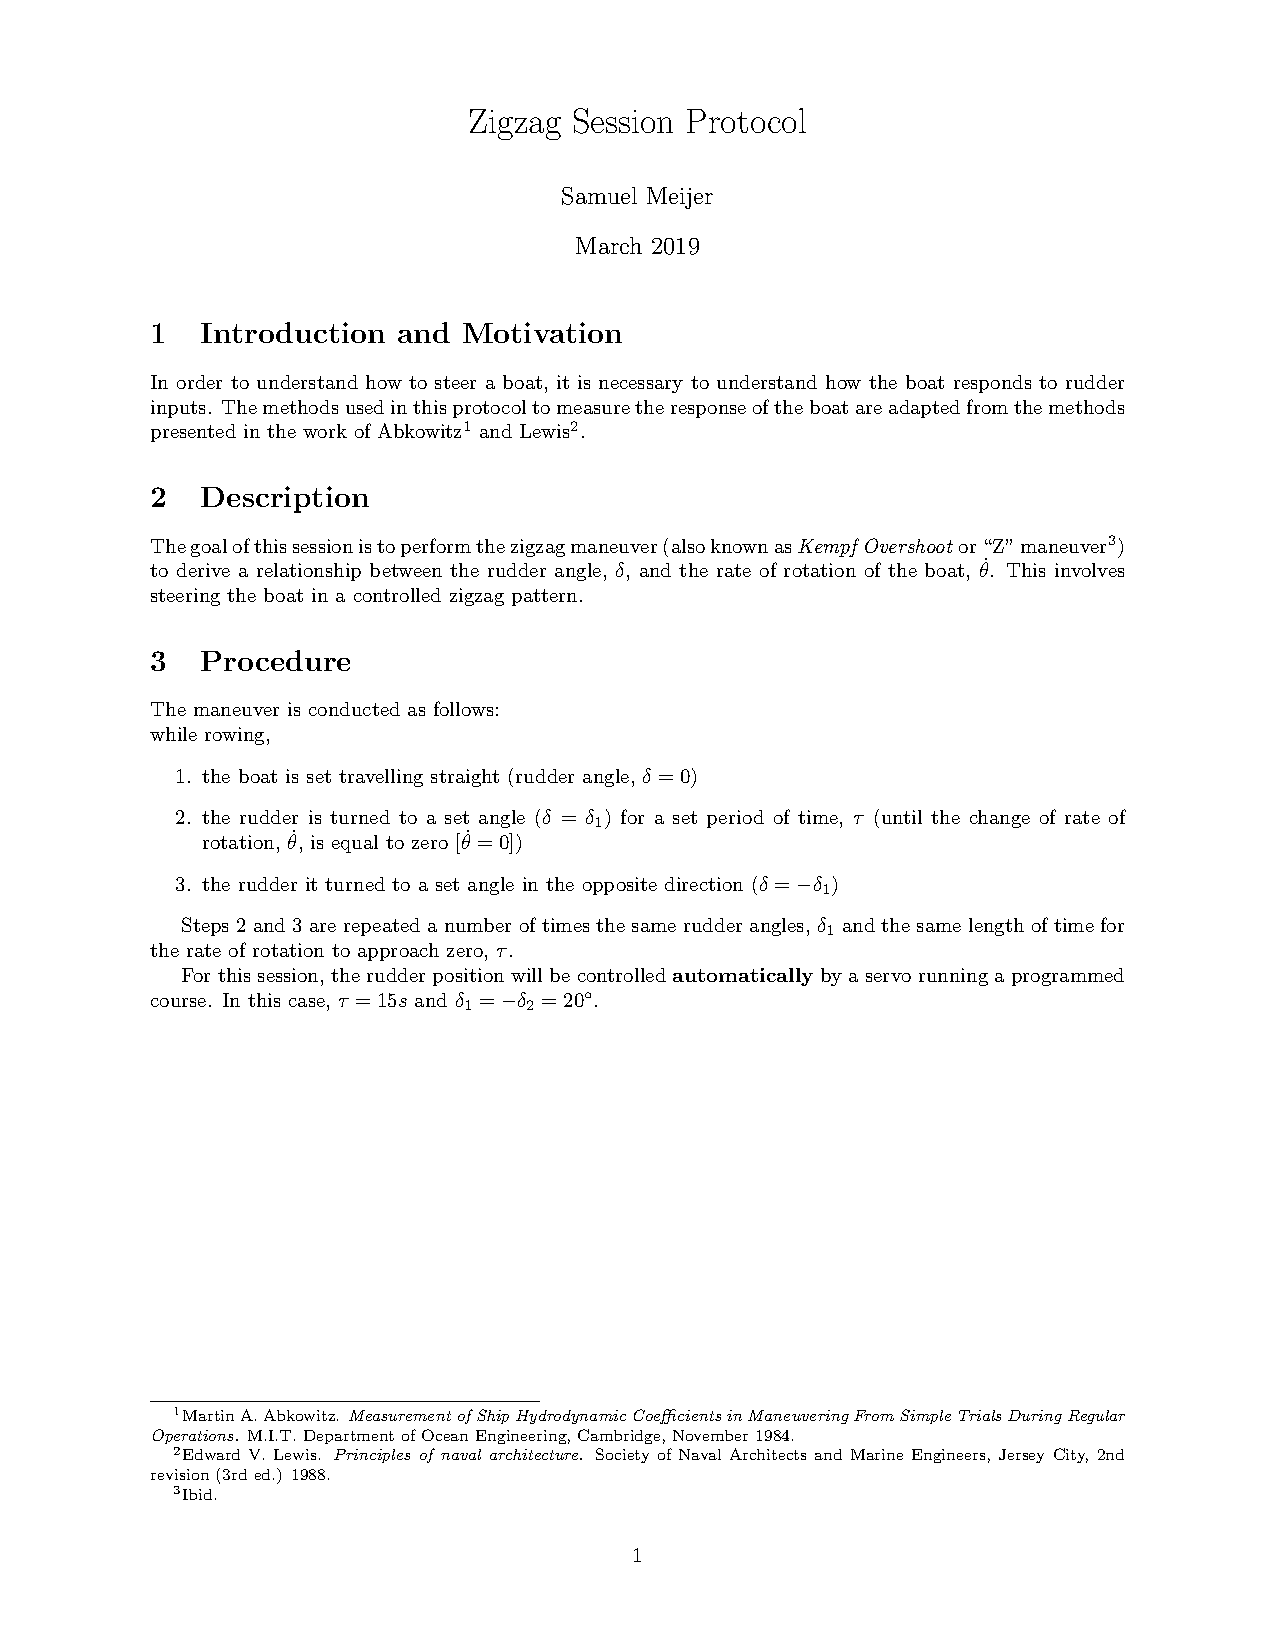
\includepdf[]{appendices/Session_Protocol-3.pdf}


% \chapter{Software}\label{app:software}
 %% You may want to include some code in your thesis. I found this method online, and would recommend you do the same... See preamble/arduinoLanguage.tex for the file that makes it look nice.
\begin{lstlisting}[language=Arduino]  
#include <Wire.h>
#include <Adafruit_Sensor.h>
#include <Adafruit_BNO055.h>
#include <utility/imumaths.h>
#include <Adafruit_GPS.h>
#include <SPI.h>
#include <SD.h>
#include <Servo.h>
#include <math.h>
#include "Filter.h"

/* This driver reads raw data from the BNO055, Potentiometer and GPS

   Connections for ADALOGGER
   ===========

   Potentiometer
   _____________
   Connect one side to VCC
   Connect other to common ground
   Connect Middle to A0

   GPS
   _____________
   Connect VIN to VCC
   Connect GROUND to common ground
   Connect GPS TX to RX1 (D0)
   Connect GPS RX to TX1 (D1)

*/

/*********************************************/
/*BNO055 (orientation) setup, variables and def'n*/
/*********************************************/
// Sample delay
const float SAMPLERATE = 10;
// Setup for the differentiation variables
double psierror = 0;
double dt = 0;
double dpsierror_dt = 0;
double previouspsierror = 0;

\end{lstlisting}

\end{document}